\documentclass[12pt, a4paper, twoside]{book} % twosided document

\author{Ana Lucia Castro}
\title{\textbf{Un encuentro de arte y terapia}}
\date{}

\let\cleardoublepage=\clearpage
\setcounter{tocdepth}{1} % Do not show sections in TOC

% ---------------- Packages ----------------
\usepackage{graphicx}
\graphicspath{{./images/}}

\usepackage{caption}
%\captionsetup[figure]{font=small,labelfont=small}
\captionsetup[figure]{labelformat=empty} % no label line

\usepackage[utf8]{inputenc}
\usepackage[spanish]{babel}

\usepackage{chngcntr}
\counterwithout{figure}{chapter}

\usepackage{csquotes}
\usepackage{float}

\usepackage[scaled]{helvet}
\renewcommand{\familydefault}{\sfdefault} % Helvetica as default

\usepackage{fancyhdr}
\pagestyle{fancy}
\fancyhf{}
\fancyfoot[C]{\thepage}  
\renewcommand{\chaptermark}[1]{}
\renewcommand{\sectionmark}[1]{}

\usepackage{tikz}
\usepackage{eso-pic} % place TikZ picture on every page

\definecolor{strongbeige}{RGB}{222,184,135} % warm, noticeable beige
\definecolor{slightlylighter}{RGB}{238,214,175} % just slightly lighter for subtle gradient

% Background gradient command
\newcommand\BackgroundGradient{%
  \begin{tikzpicture}[remember picture,overlay]
    % Very subtle gradient: strong beige to slightly lighter
    \shade[top color=strongbeige,bottom color=slightlylighter!20]
      (current page.south west) rectangle (current page.north east);
  \end{tikzpicture}%
}
%
% ---------------- Document ----------------
% Change the size of normal text only
\makeatletter
\renewcommand\normalsize{%
   \@setfontsize\normalsize{13pt}{15pt} % font size, line spacing
}
\makeatother

\AddToShipoutPictureBG{\BackgroundGradient}

\begin{document}

% Title page
\maketitle
\thispagestyle{empty} % no header/footer

% Table of contents
\tableofcontents

% Chapter 1
\chapter{La mujer resignificada}

\begin{figure}[H]
	\centering
	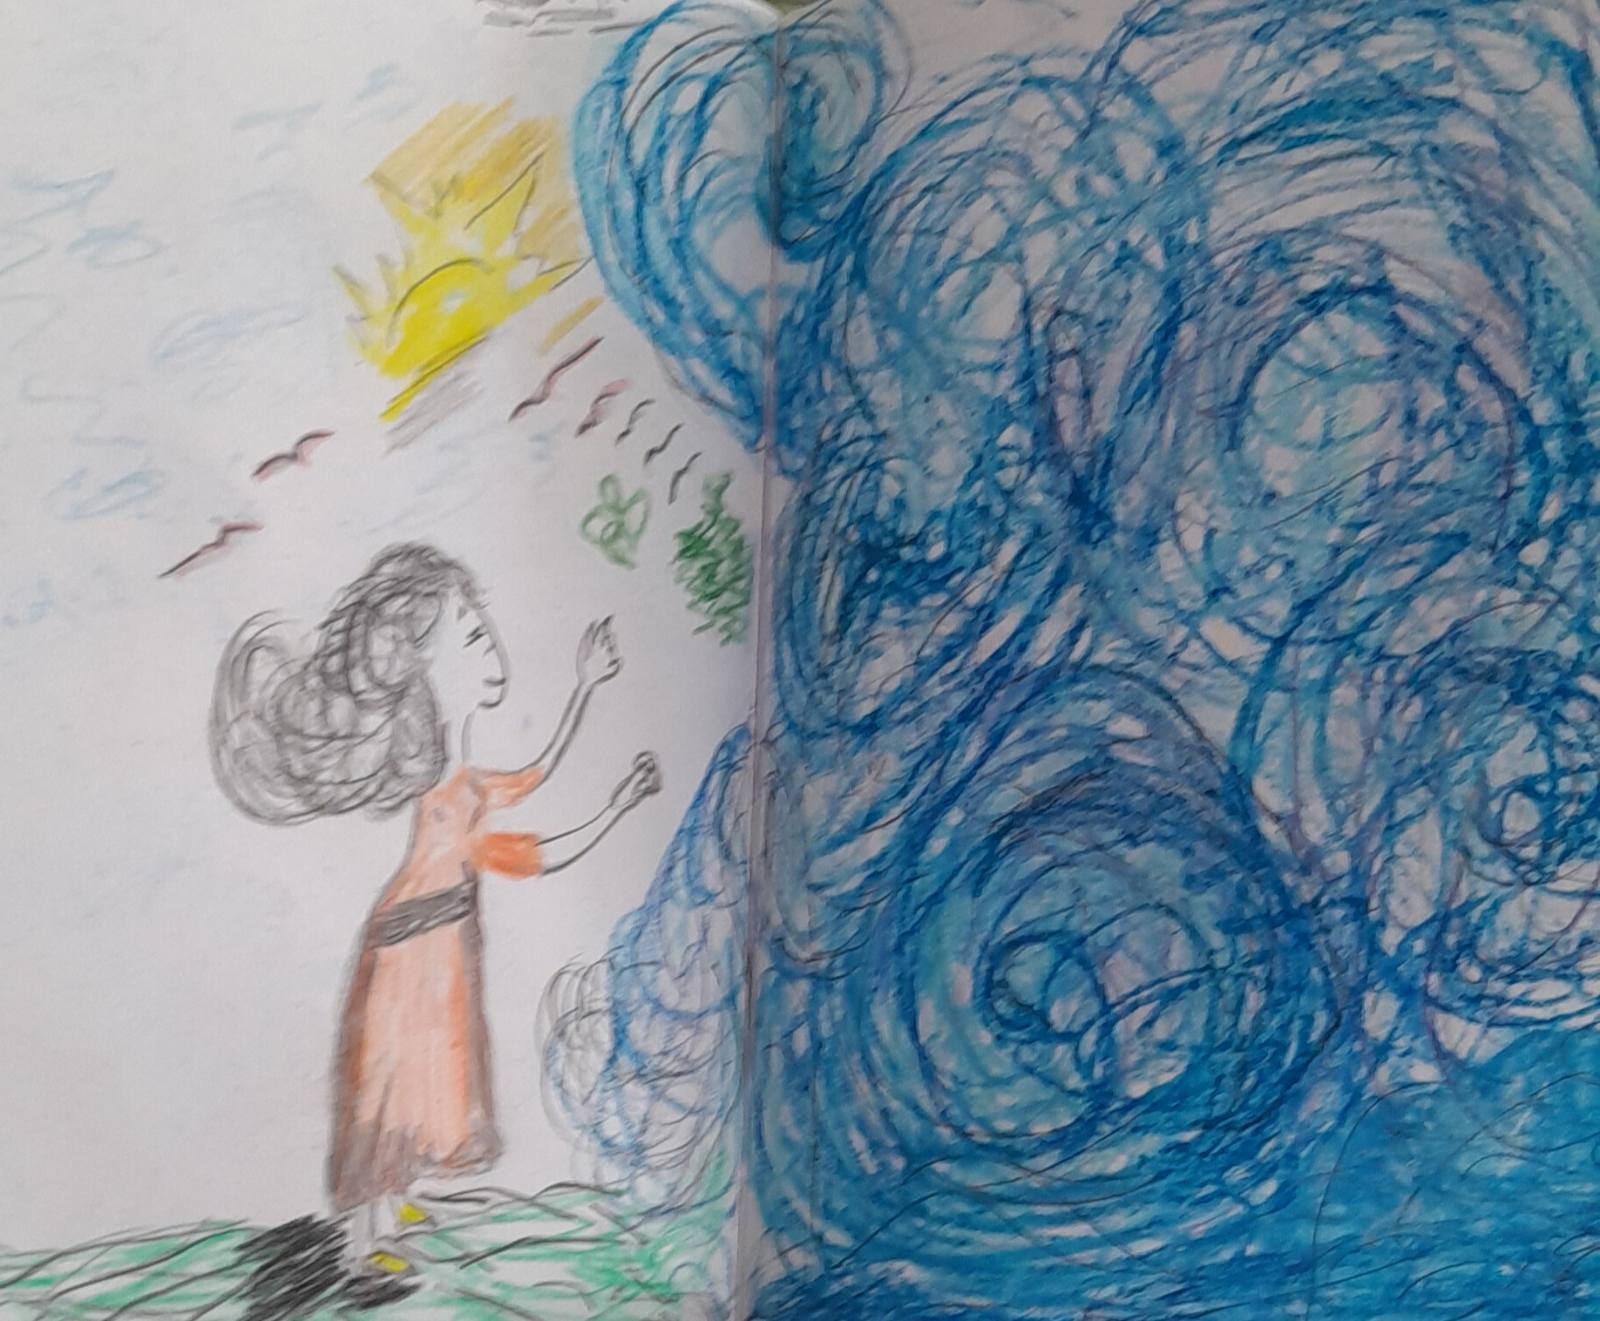
\includegraphics[width=\textwidth]{./images/1f81324df3940b.jpg}
\end{figure}

\clearpage

\noindent\textbf{Hoy decido}\\
Hoy decido ser la mujer sabia\\
Hoy decido en la flor de loto estar sentada\\
Hoy decido por los hombres que decidieron mi sumisión\\
Hoy decido hacer pequeñito a aquello que la degrado\\
Al puerco poseído mandarlo a su abismo, al doctor que sugirió acunar al patriarcado mandarlo a pastar el  ocaso de su ganado\\
Hoy decido contemplar las oportunidades de mis alas\\
Decido por todas aquellas esperanzas que se contemplaron en danzas, llamando por decadas para  ser escuchadas\\
Como le digo a mi adolescente que de doler se cuese y que a ella le tocó esa batalla?\\
Que se quede tranquila por que hoy ya no la encausan, ella venera su dignidad y no espera que un potro la monte para sentir que confirma su feminidad.\\
Sostengo este malestar y en mi vientre lo modelo, moldeo como el útero que no fue creado, sostengo en mi angustia de garganta este feto y  como todas las derrotas que duelen, acepto,acepto ser lo que soy  y luego...que aparezca el espacio, la crisis, los opuestos, mientras siga eligiendome desde lo sincero, en nombre de la realidad desde lo pequeño hasta lo que se hace eterno.\\
Hoy elijo ser una mujer más que contempla su duelo! Que de suertes ya la baraja estaba asignada, que por esto los trucos son hoy para mi una ventaja, Por lo menos no seré la mujer que por ser madre se ve fracasada,  de sus sueños y anhelos sepultada...sino que puedo encausar mi mirada a la señora que por si misma se sostiene y elije... hoy elijo  ser resignificada!

\begin{figure}[H]
	\centering
	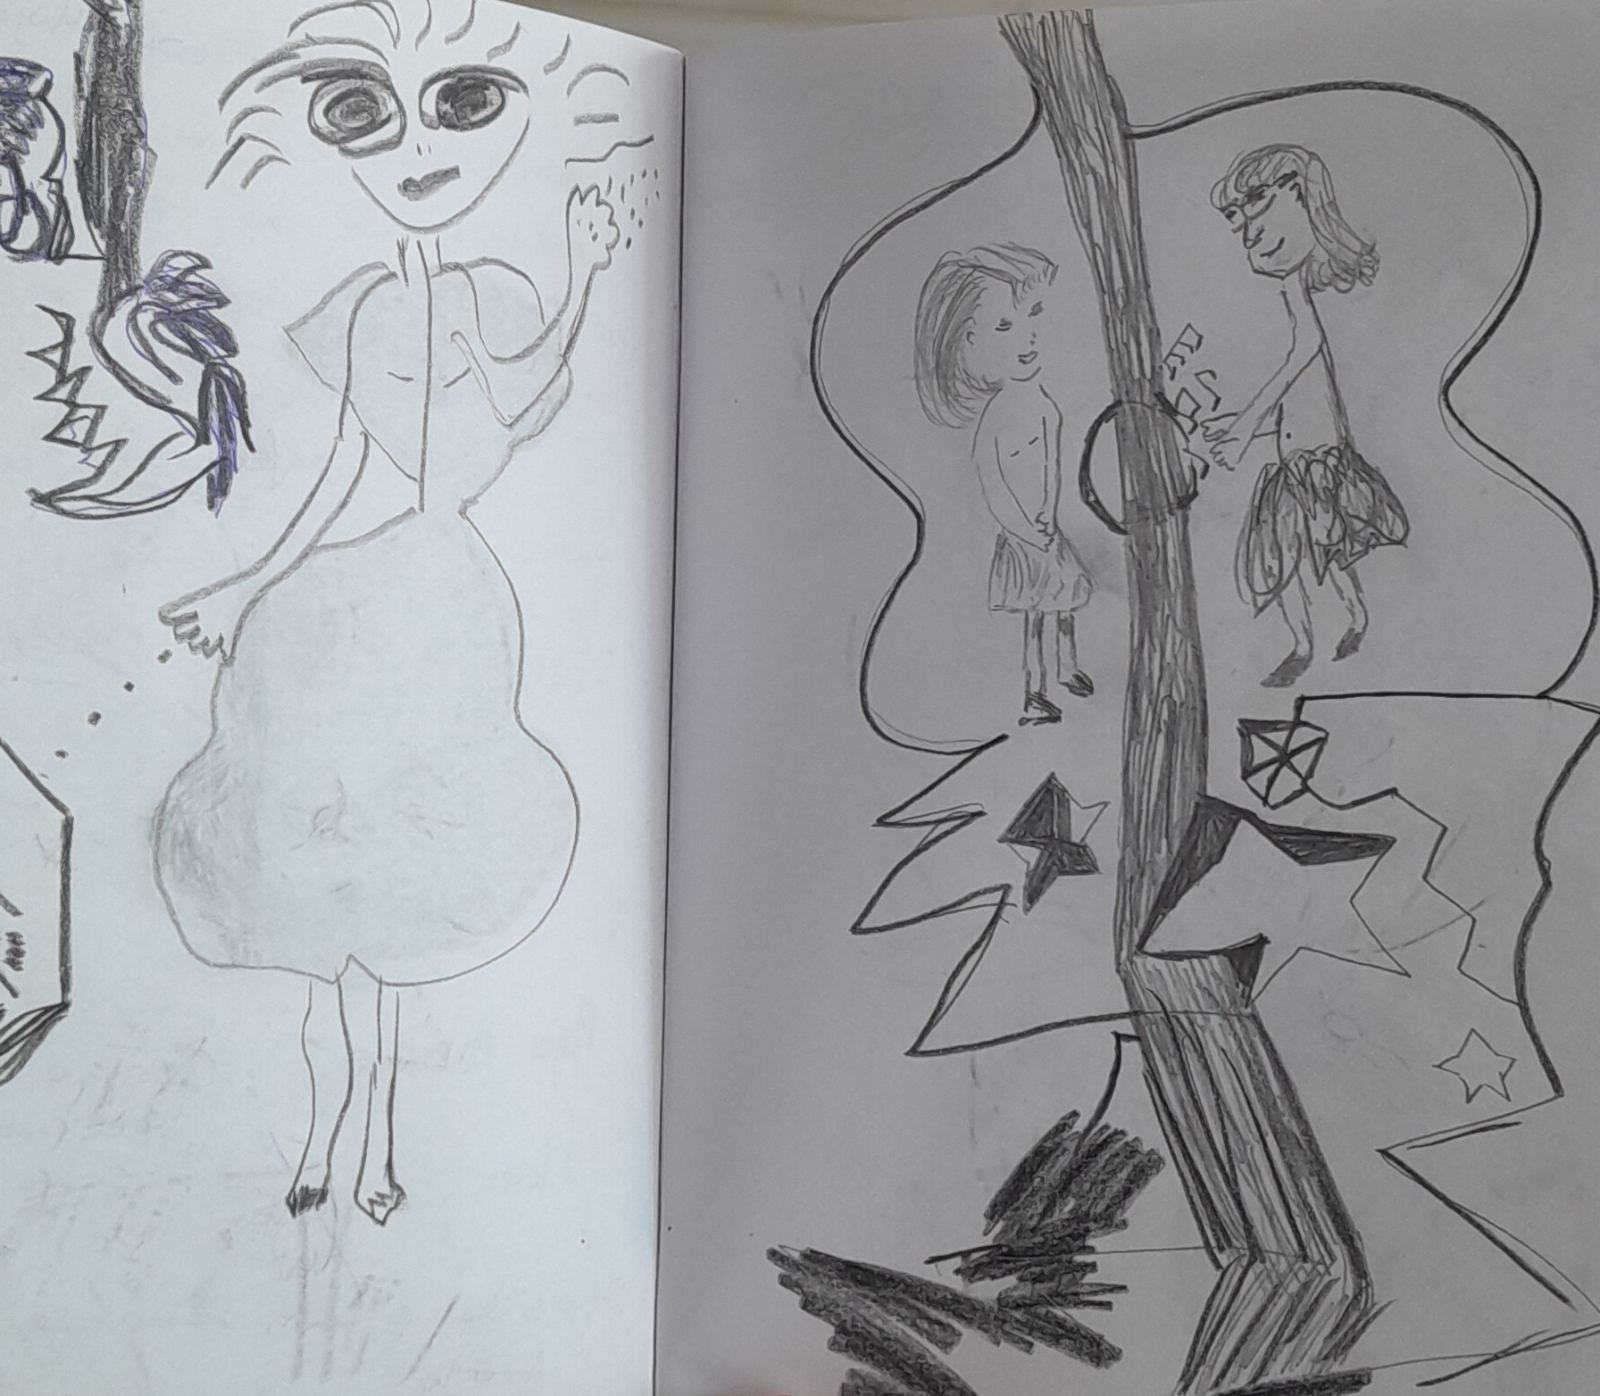
\includegraphics[width=\textwidth]{./images/1f81324df24ae9.jpg}
\end{figure}

\begin{figure}[H]
	\centering
	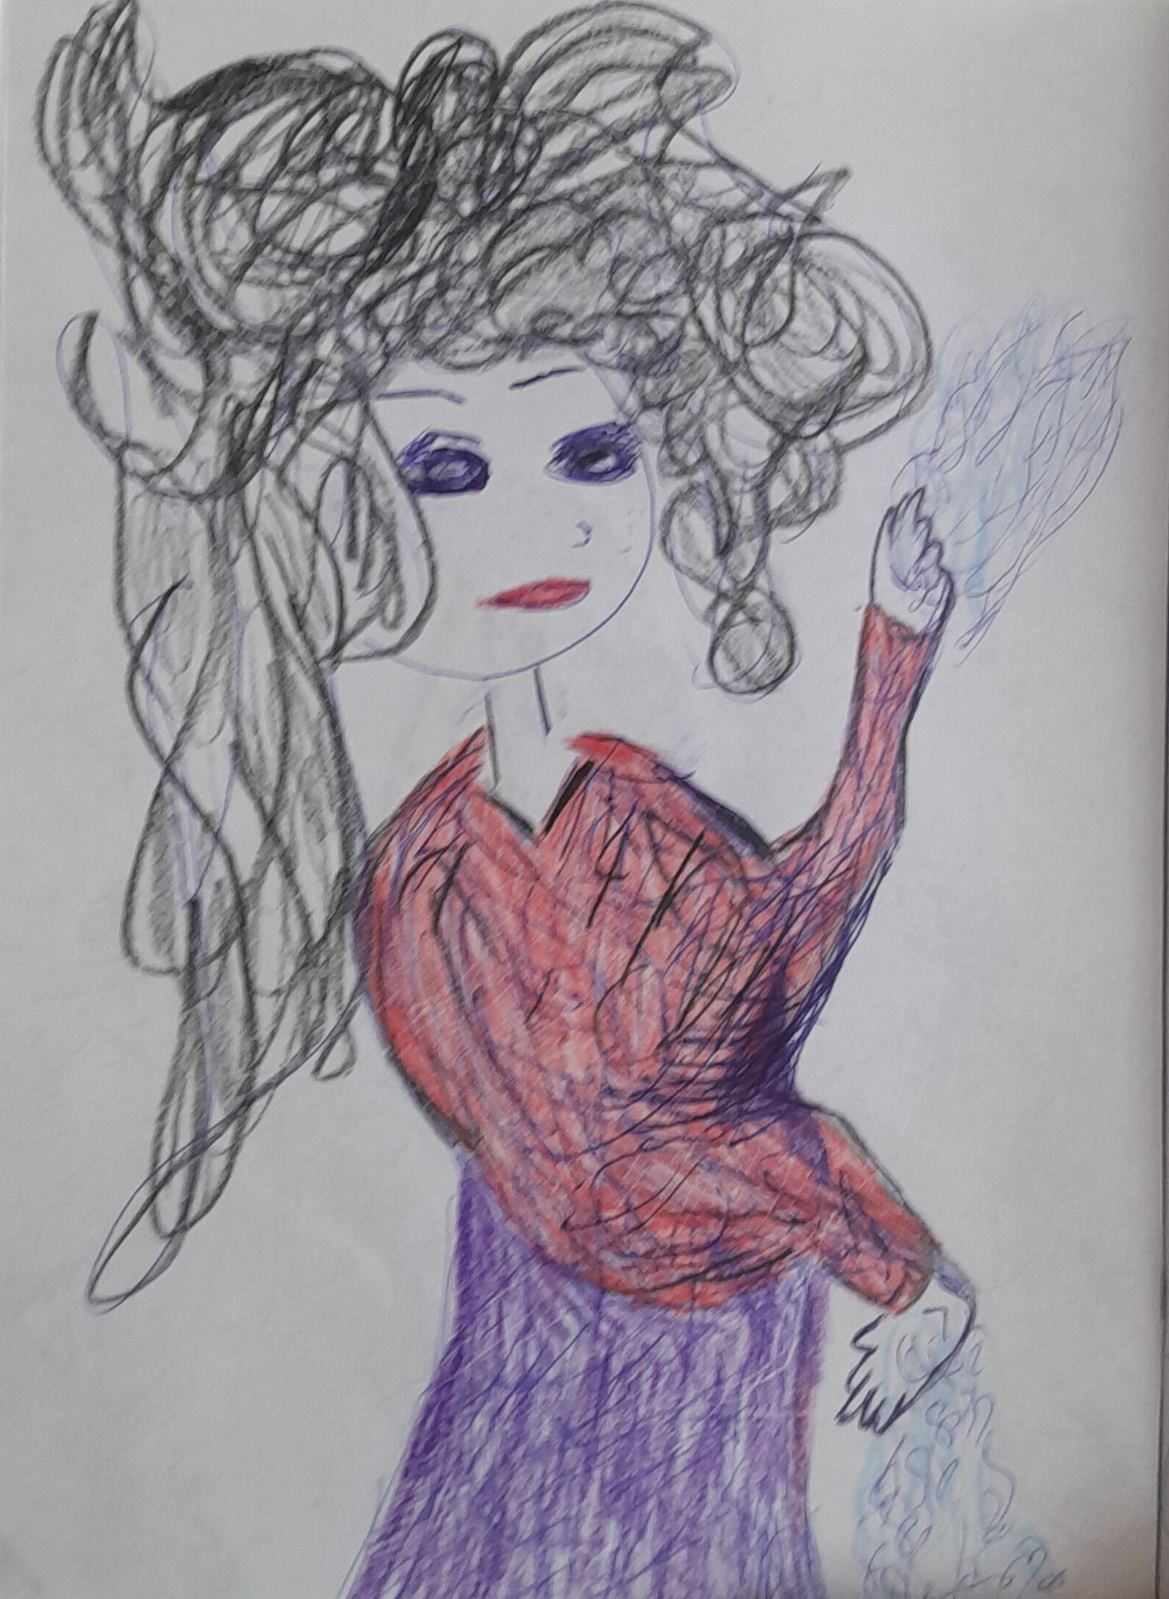
\includegraphics[width=\textwidth]{./images/1f81324df206df.jpg}
\end{figure}

\clearpage

\noindent\textbf{Entre la que fui, entre la que soy}\\
Mientras bailaba, me sentí observada, no es que no lo haya experimentado antes, es que ahora bailo hacia adentro.\\
Improvisaba pasos de los que he aprendido, sin embargo no era el mismo el cuerpo que me acompañaba, he añorando que se parezca, el cambio parace ser de atractivo a elegante.\\
Míentras bailaba lo hacia por una cuerda floja, que se balanceaba entre lo que fui entre lo que soy, la línea estrecha, a lo lejos se veia  infinita.\\
Mientras bailaba mis pasos requerian de más cuidado, ni para la izquierda ni muy a la derecha,por el centro y en puntas de pie, encontrando y reconociendo el nuevo ritmo.\\
Hoy me sentí observada mientras bailaba y el ojo no era ni de un juez ni de un justiciero, sino del que todo lo vela.\\
Ya no bailaba para la atracción ni para mis caprichos o en la ilusión, quise bailar sin ser alabada, y que mujer he visto en el espejo, se escondía de a ratos y luego se elevaba.\\
Seguiré bailando cada una de las etapas.

\clearpage

\begin{figure}[H]
	\centering
	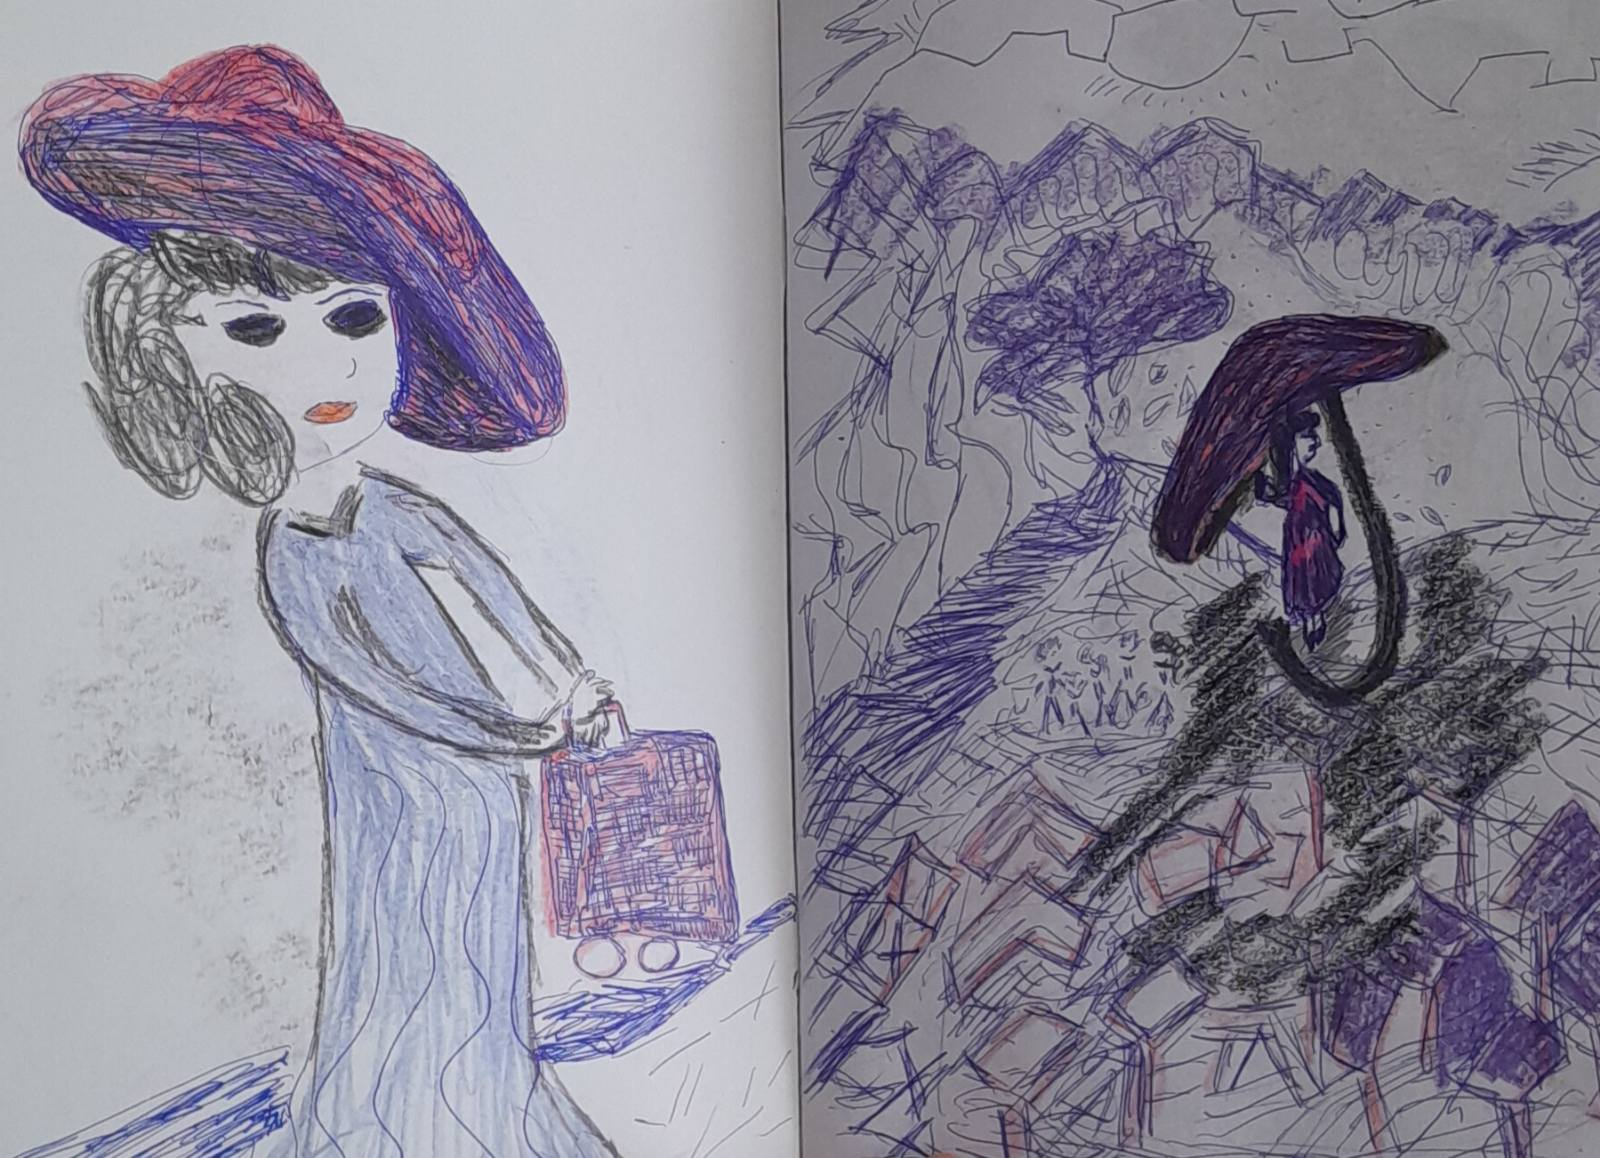
\includegraphics[width=\textwidth]{./images/1f81324df23788.jpg}
\end{figure}

\clearpage

\noindent\textbf{La voz y la espada}\\
La de su padre, la princesa como solían llamarla, cantaba y bailaba y a todos enamoraba, con su inocencia, sus ojos transparentes, la eterna niña en un cuento de hadas...
Rodeada de seres que la respetaban, junto al torso bien ancho del rey de la manada, el hombre inmenso, omnipotente el que sus sueños más profundos con su tridente resguardaba.
No habría nadie que se interpusiera a tal admiración, ni siquiera la mujer devoradora los alejaba de esa unión.
Cuenta la leyenda que un día salió la princesa de su refugio para ayudar a otros, el cual era su secreto oculto, y en el reflejo de un hombre pudo contemplar su ser.
Quedó tan enamorada, ilusionada que no dudó en querer estar con él, y aunque él se veía diferente a su padre, añoraba con poder con ese príncipe comunicarse, fue ahí que descubrió que el no podía escuchar su voz...
Decidió recurrir a su padre para entender la cuestión, su padre con pocas palabras el trasfondo le reveló, generaciones de mujeres solo escucharon una voz, y esa voz que ella conoce y que cuida con amor no funciona en otros reinos, sea clara la intención. Resurgió en ella tal enfado, algo que jamás había experimentado y sin pensarlo fue a ver a esa mujer, la que tanto había negado, le pregunto si habría un hechizo que revelará una nueva voz...la señora envidiosa no dudó ni un sopetón en cambiarle la voz de un ángel por una que entre hombres sea aclamada, así  fue que cambio la princesa su don por una espada.
Que podría hacer con esa espada se preguntaba ella entusiasmada.

\clearpage

Hasta que volvió al encuentro con el hombre que amaba y se paró frente a él en movimientos de ataque, el príncipe esos lenguajes manejaba, así que no dudó en intentar defenderse, así danzaron juntos hasta que se hizo la noche, cansados, agotados durmieron juntos en un bote.
Al día siguiente lo mismo, ella aceptaba ese diálogo, él no entendía, pero tampoco otro conocía.
Duraron semanas y años, hasta que la princesa comenzó a extrañar su canjto, él ya se había acostumbrado, ella se iba marchitando en cambio.
Un día escucho el tridente en forma de truenos, ahí supo que era momento, el hechizo habria terminado.
Decidió volver a la profundidad, volvió a ver a sus amigos, su seguridad y su padre la abrazo esperanzado.
Pasaron de nuevo los años, su voz ya ni siquiera era su valor...nada la reconfortaba.
Que le sucede a la princesa preguntaban?
Tras una noche de sueños que su padre velaba, apareció aquel príncipe en forma de  hada...
Que deseas princesa para despertar? Deseo conocer mi esencia sin volverme a engañar.
Entonces caminemos juntas, te voy a ayudar...y quién eres tú si puedo saberlo?
Soy la Madre que has buscado, la madre del Universo.

\clearpage

\begin{figure}[H]
	\centering
	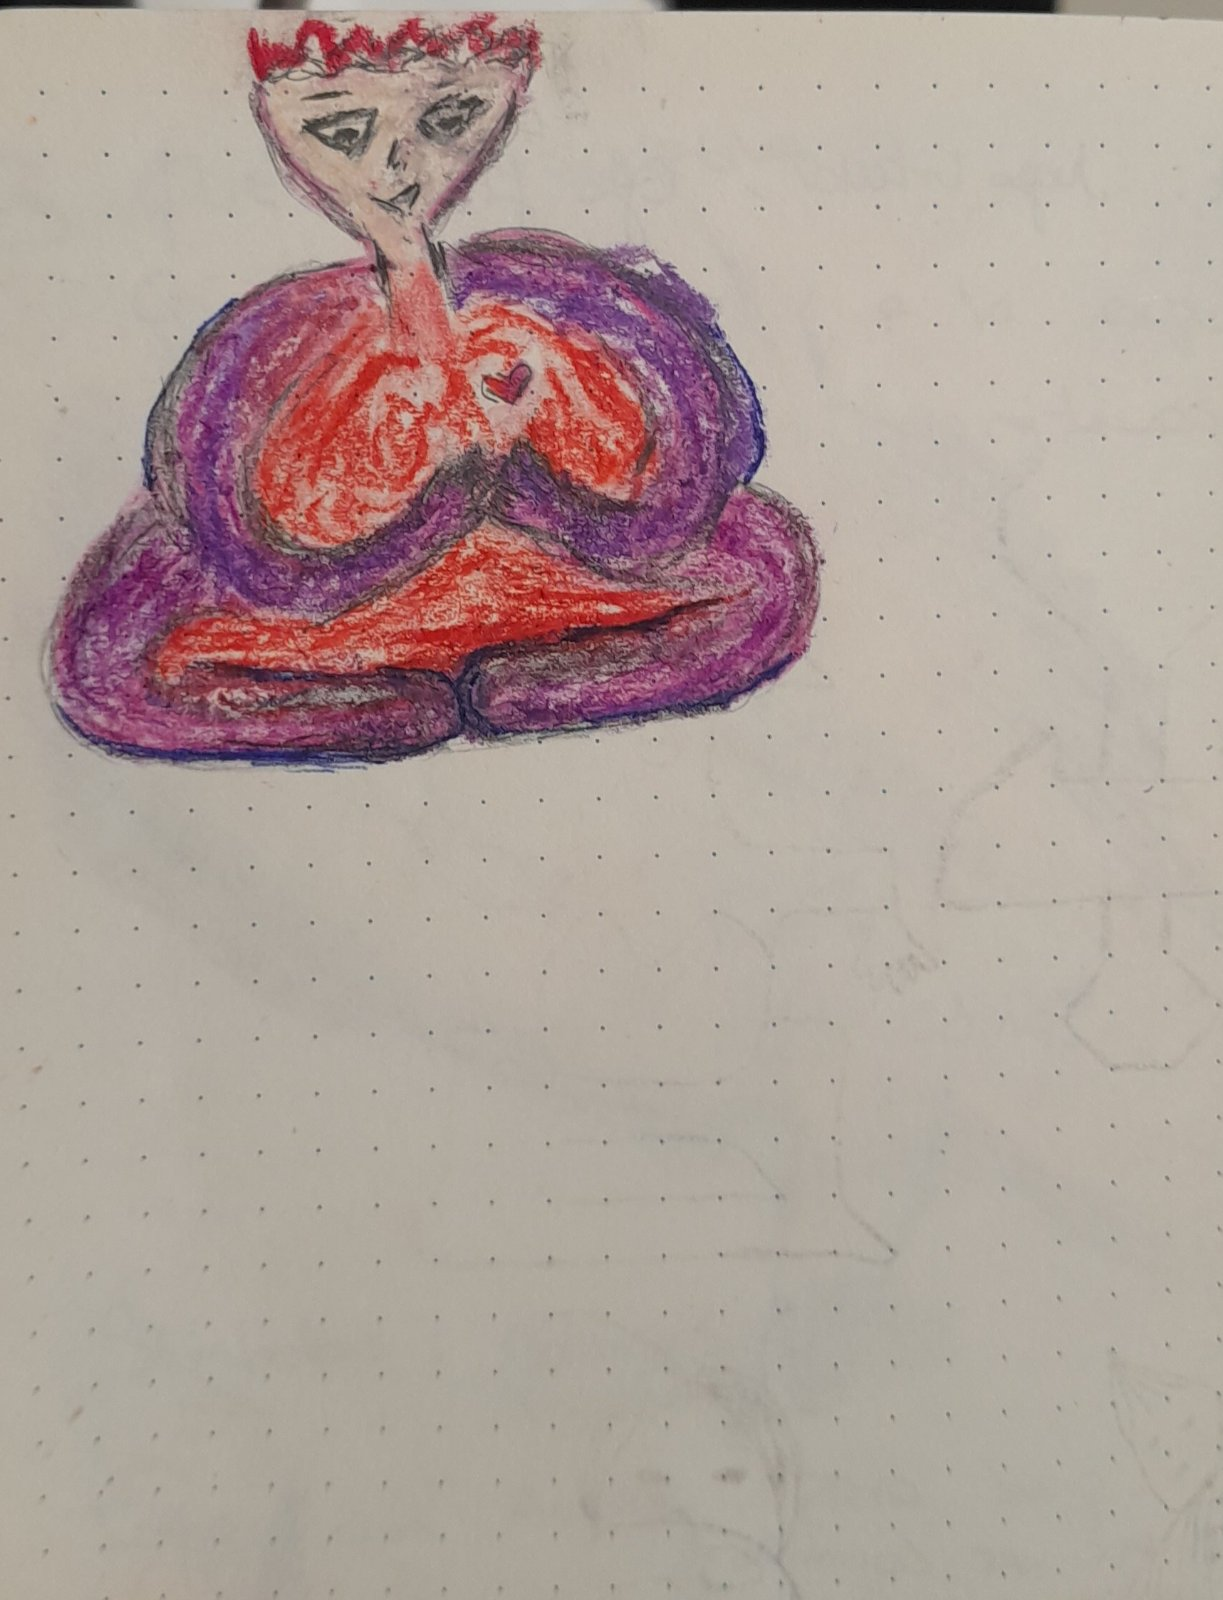
\includegraphics[width=\textwidth]{./images/1f81324dd8f012.jpg}
\end{figure}

\begin{figure}[H]
	\centering
	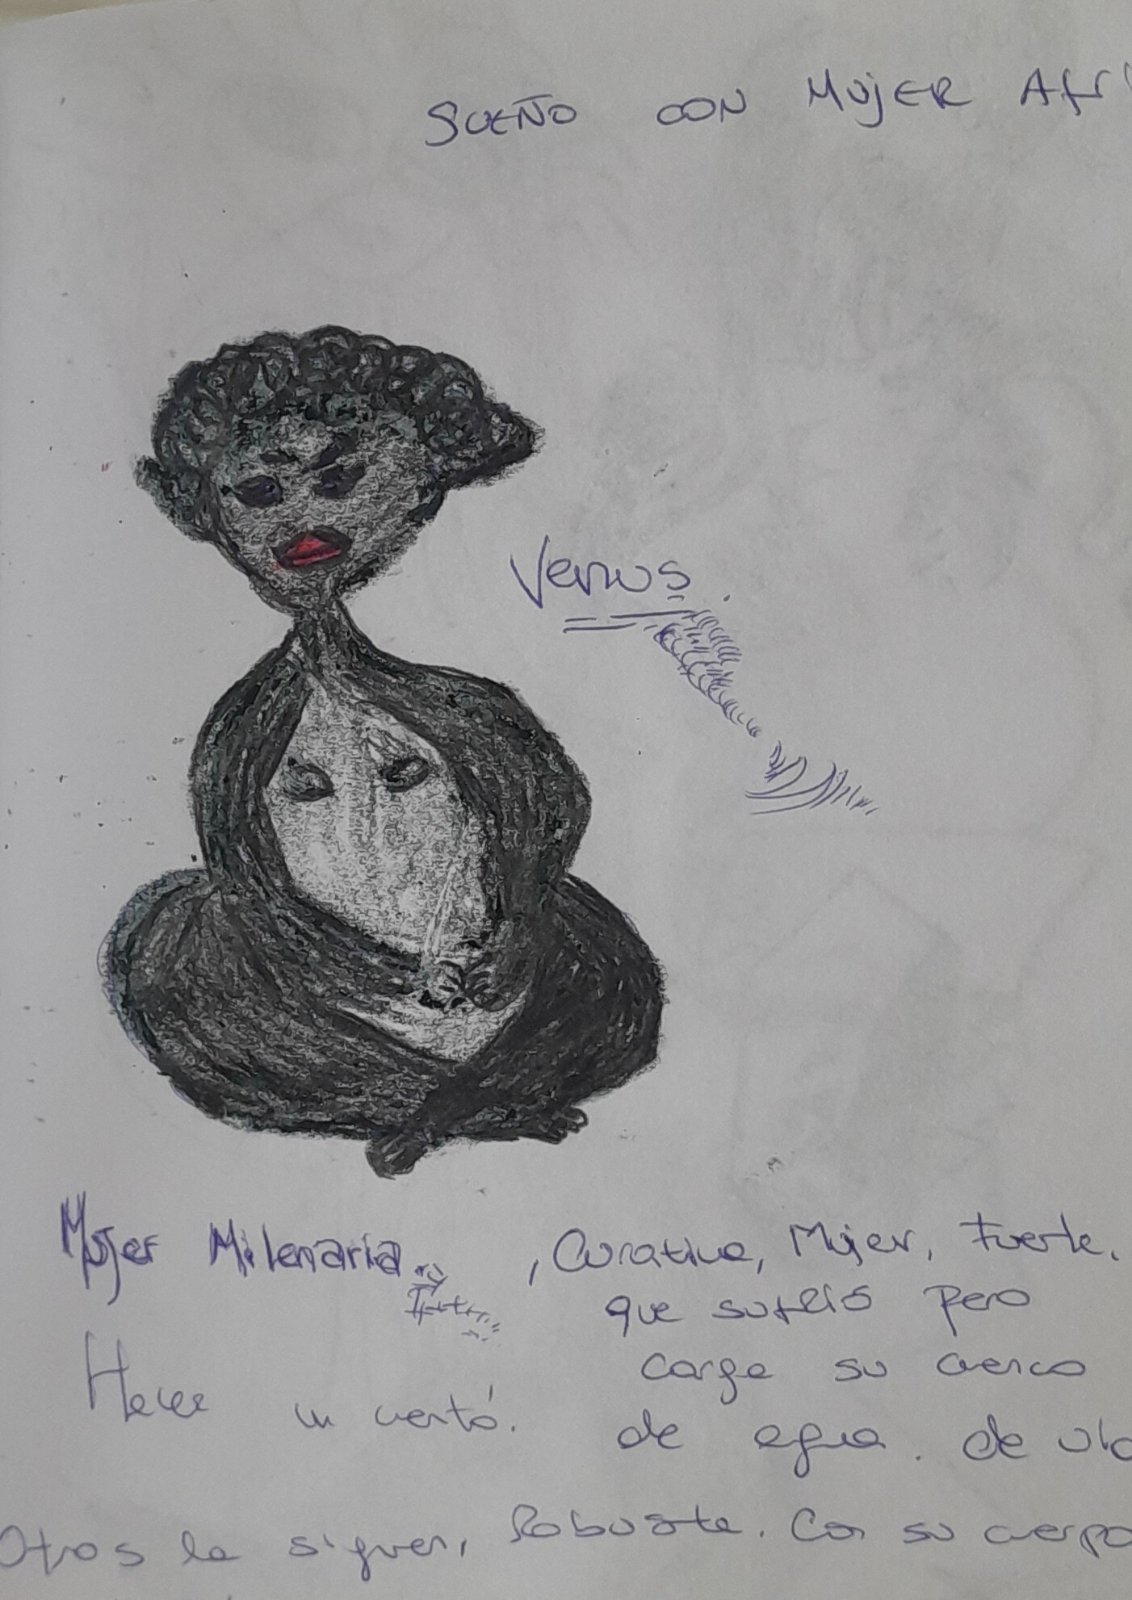
\includegraphics[width=\textwidth]{./images/1f81324df27a62.jpg}
\end{figure}

\clearpage

\noindent\textbf{Mujer}\\
De sumisa a Artemisa en su mirada, de apasionada con la vida a la mansa que cuida de su morada.\\
La que respira nuevas esperanzas y llora por la desgracia que calla,\\
la que vive y muere en cada etapa.\\
La que a veces se enamora de ella misma y a la vez necesita un macho alfa que la vuelva loca.\\
La que se rige con la dignidad de una leona y es un cachorrito asustado cuando de energías extrañas se trata.\\
La que protege como una fiera, la que necesita protección como un ambriento niño huérfano\\
La que peca con su imaginación y de su intuición no sospecha.\\
La que amanece en otra estratosfera recontandose sus sueños, con otra vida, otras historias.\\
La mujer que quiere comerse al mundo y se refugia en su castillo.\\
La que se entretiene en la muchedumbre, la que se rescata a solas entre cuentos de hadas.\\
La mujer virgen, sabía, inmaculada, también la callejera desalmada encubriendo en sentimientos de amor necesidades desenfrenadas.\\
La que mucho conoce y a su vez se desconoce;reprimida y empoderada.\\
La que lucha por no hacer nada, y a la vez fluir con lo que está predestinado, la que se sumerge entre dudas acertadas.\\
La mujer que se sintió desvalorizada y tiene el valor para ser reparada.\\
La mujer que ingiere pero no traga, que a escondidas llora un amor adolescente, una ausencia de útero que la desgarra, que sangra por otras vertientes y ni una gota de sangre la acompaña.\\
Lo estamos todas juntas logrando!!!

\clearpage

\noindent Mujer por otros aclamada y por ella misma tan maltratada.\\
Mujer!!! Te necesito mujer!!!\\
Reconfigurame en obras de arte, aunque sean un desastre.\\
Háblame con la verdad, sin caretas ni dizfrases\\
Escupeme en la cara tu odio, un sentimiento que vive y te consume en las noches, dime cuánto de infeliz eres, la que necesita reinventarse, ser escuchada, manifestarse, que todos la vean, roja como una materia que puedes manipular para bien o para mal.\\
Alimentame con el amor que te ha sido otorgado, por el omnipotente divino, acaríciame con ese instinto materno que conoces de muchas reencarnaciones.\\
Sé y fundente en la nada, como opuestos que danzan y se golpean con piedad.
Oh mujer, sé lo que eres, todas las diosas que en tu interior velan por ti, lo están intentando.

\begin{figure}[H]
	\centering
	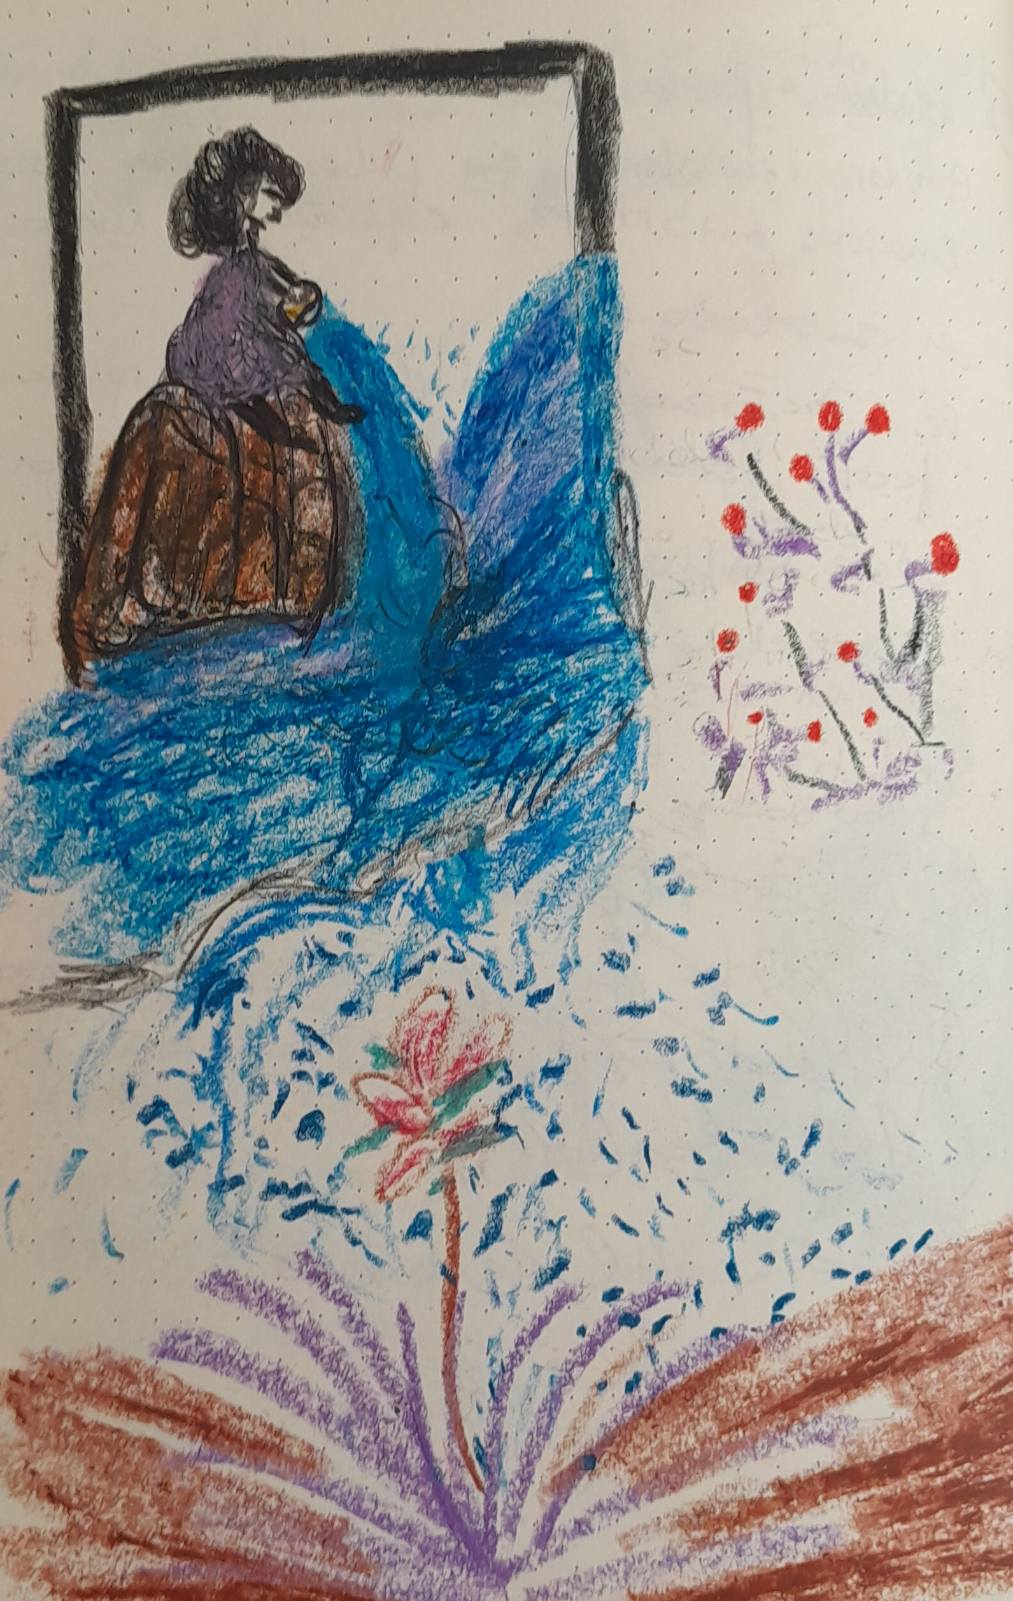
\includegraphics[width=\textwidth]{./images/1f81324dd8c5d0.jpg}
\end{figure}

\begin{figure}[H]
	\centering
	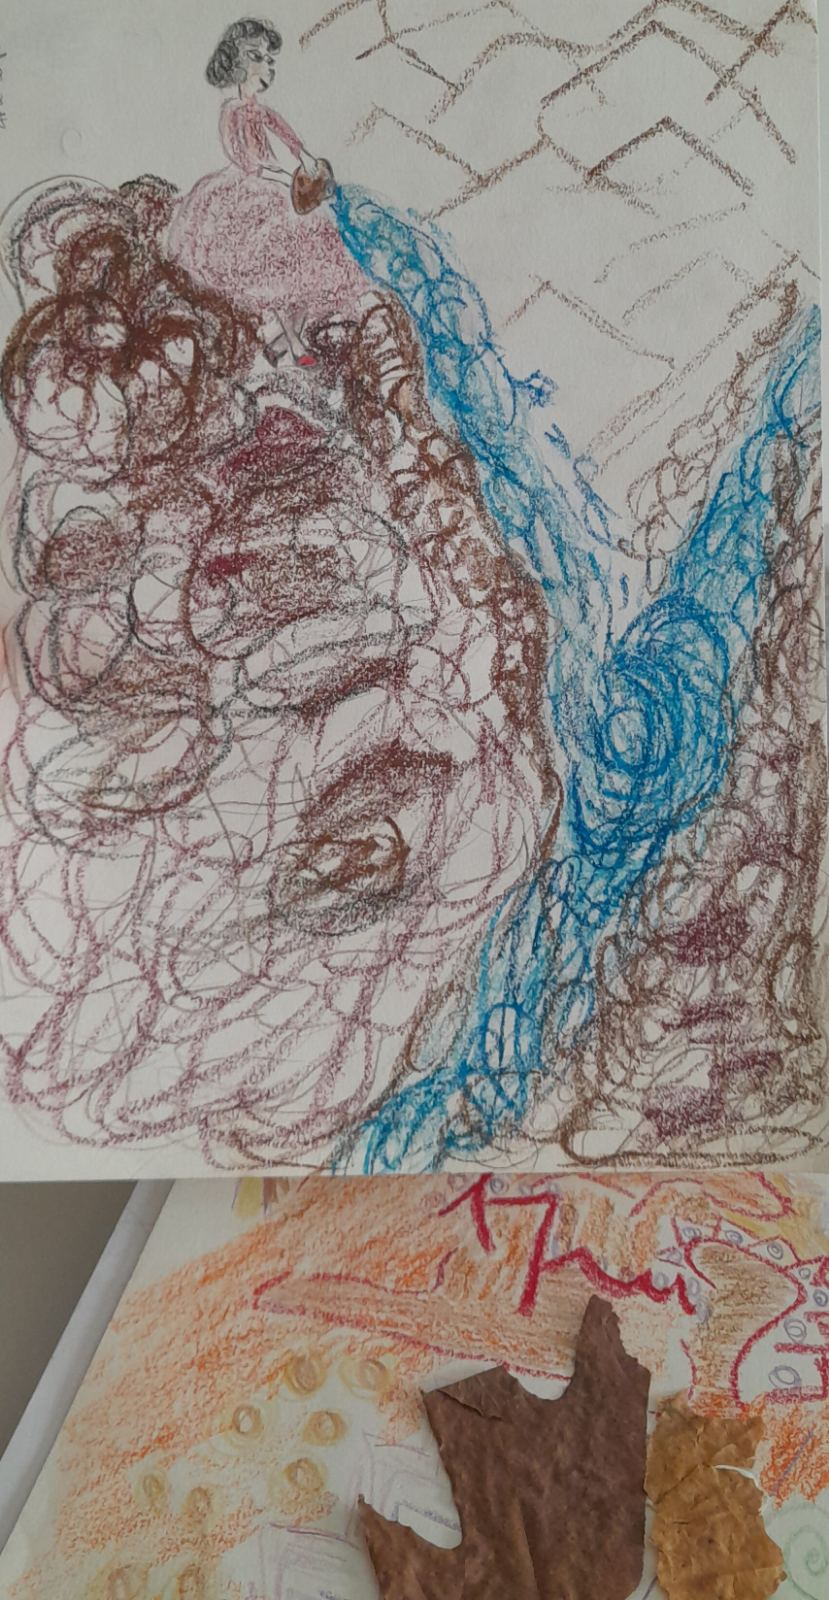
\includegraphics[width=\textwidth]{./images/1f81324df13197.jpg}
\end{figure}

\noindent\textbf{Un poder ancestral}\\
La nueva Lucia tiene energía,\\
La nueva Lucia confía en si misma\\
Se mira al espejo y una mujer ve en su reflejo\\
Le gusta estar sola y agradece a la vida\\
La nueva Lucia no necesita un amante, confía en el hombre que aparece distante\\
Soluciona sus cosas y no teme expresarse\\
Tiene padre y madre y se siente orgullosa de haber aceptado sus almas tan nobles, que le dieron todo para que no se doble\\
La nueva Lucia tiene órganos fuertes, ya no hay tal confusión que detenga su misión.

\clearpage

\begin{figure}[H]
	\centering
	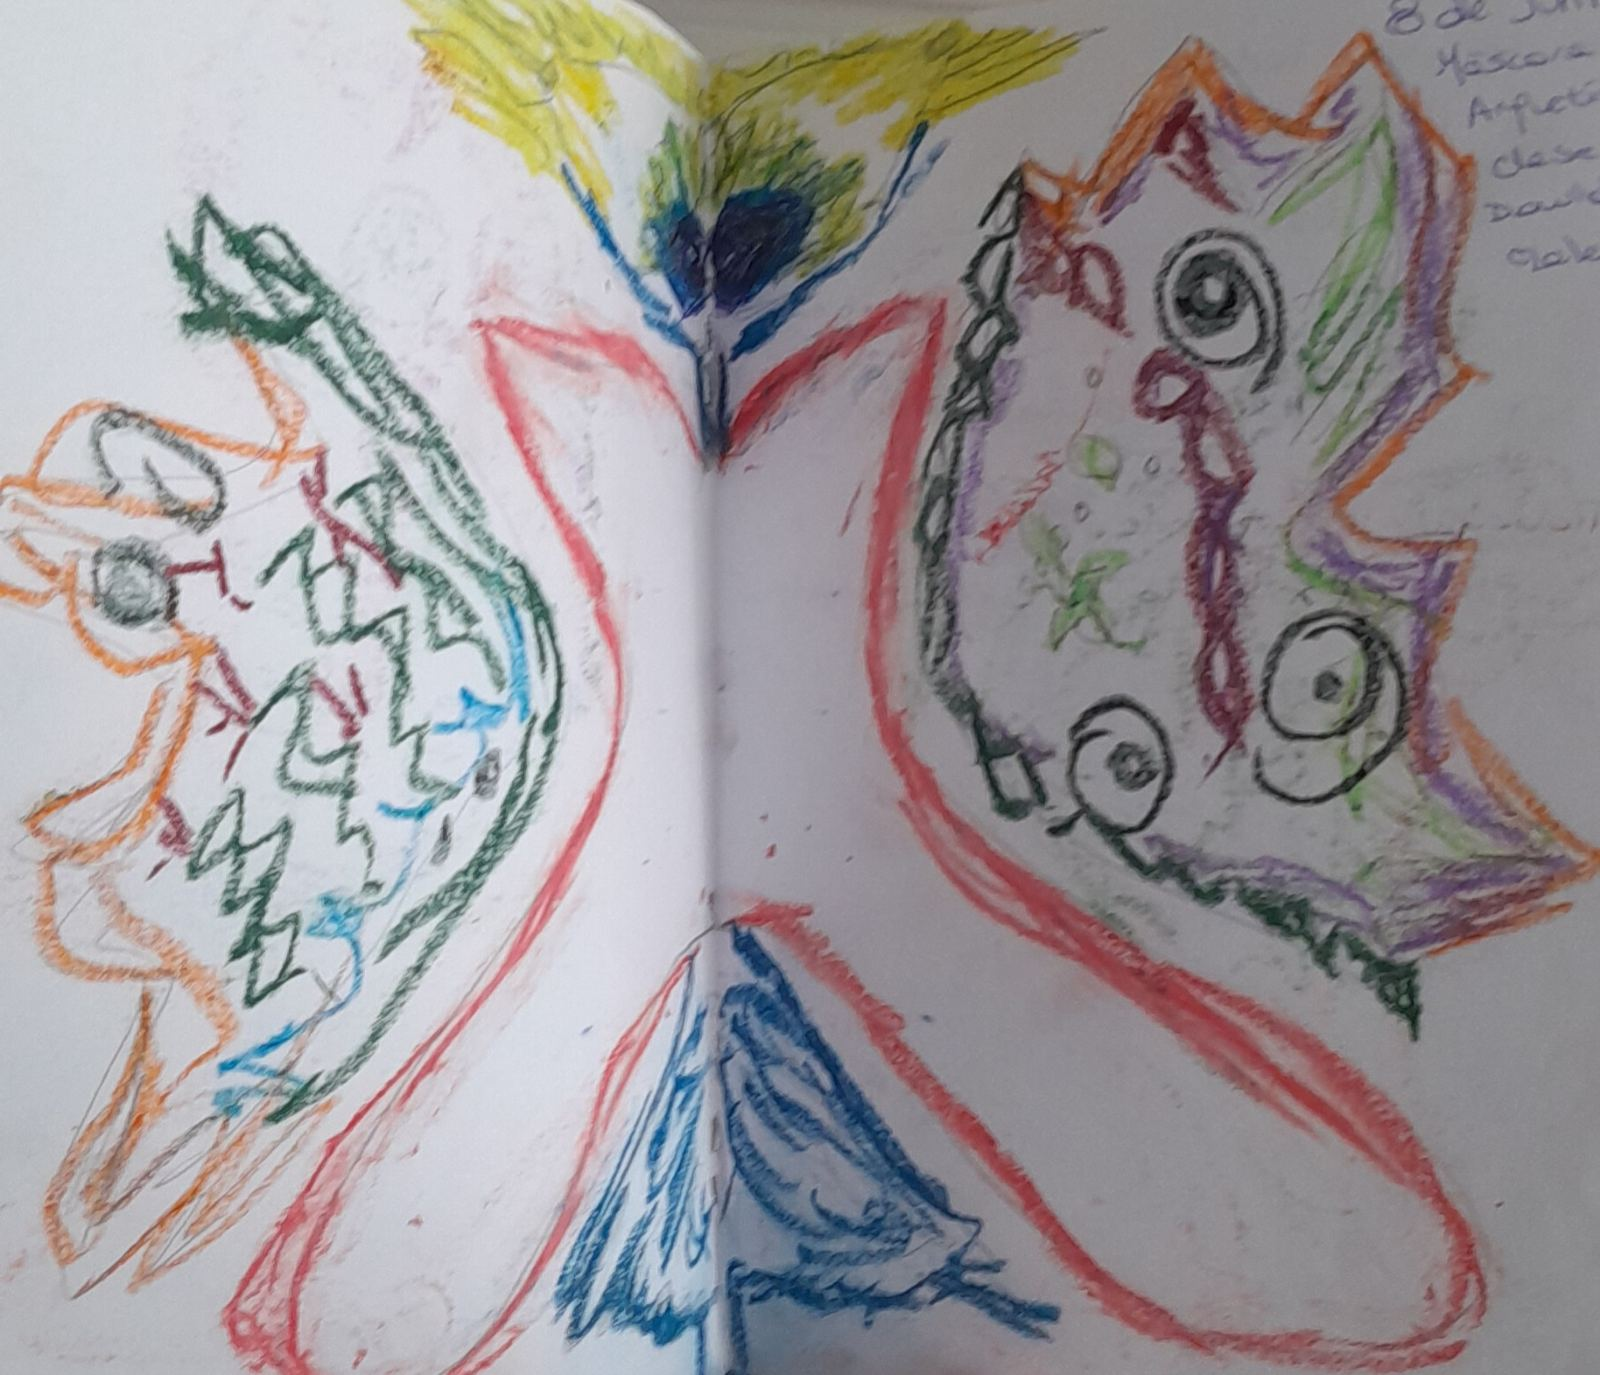
\includegraphics[width=\textwidth]{./images/1f81324df39a29.jpg}
\end{figure}

% Chapter 2
\chapter{De madre a Madre}

\begin{figure}[H]
	\centering
	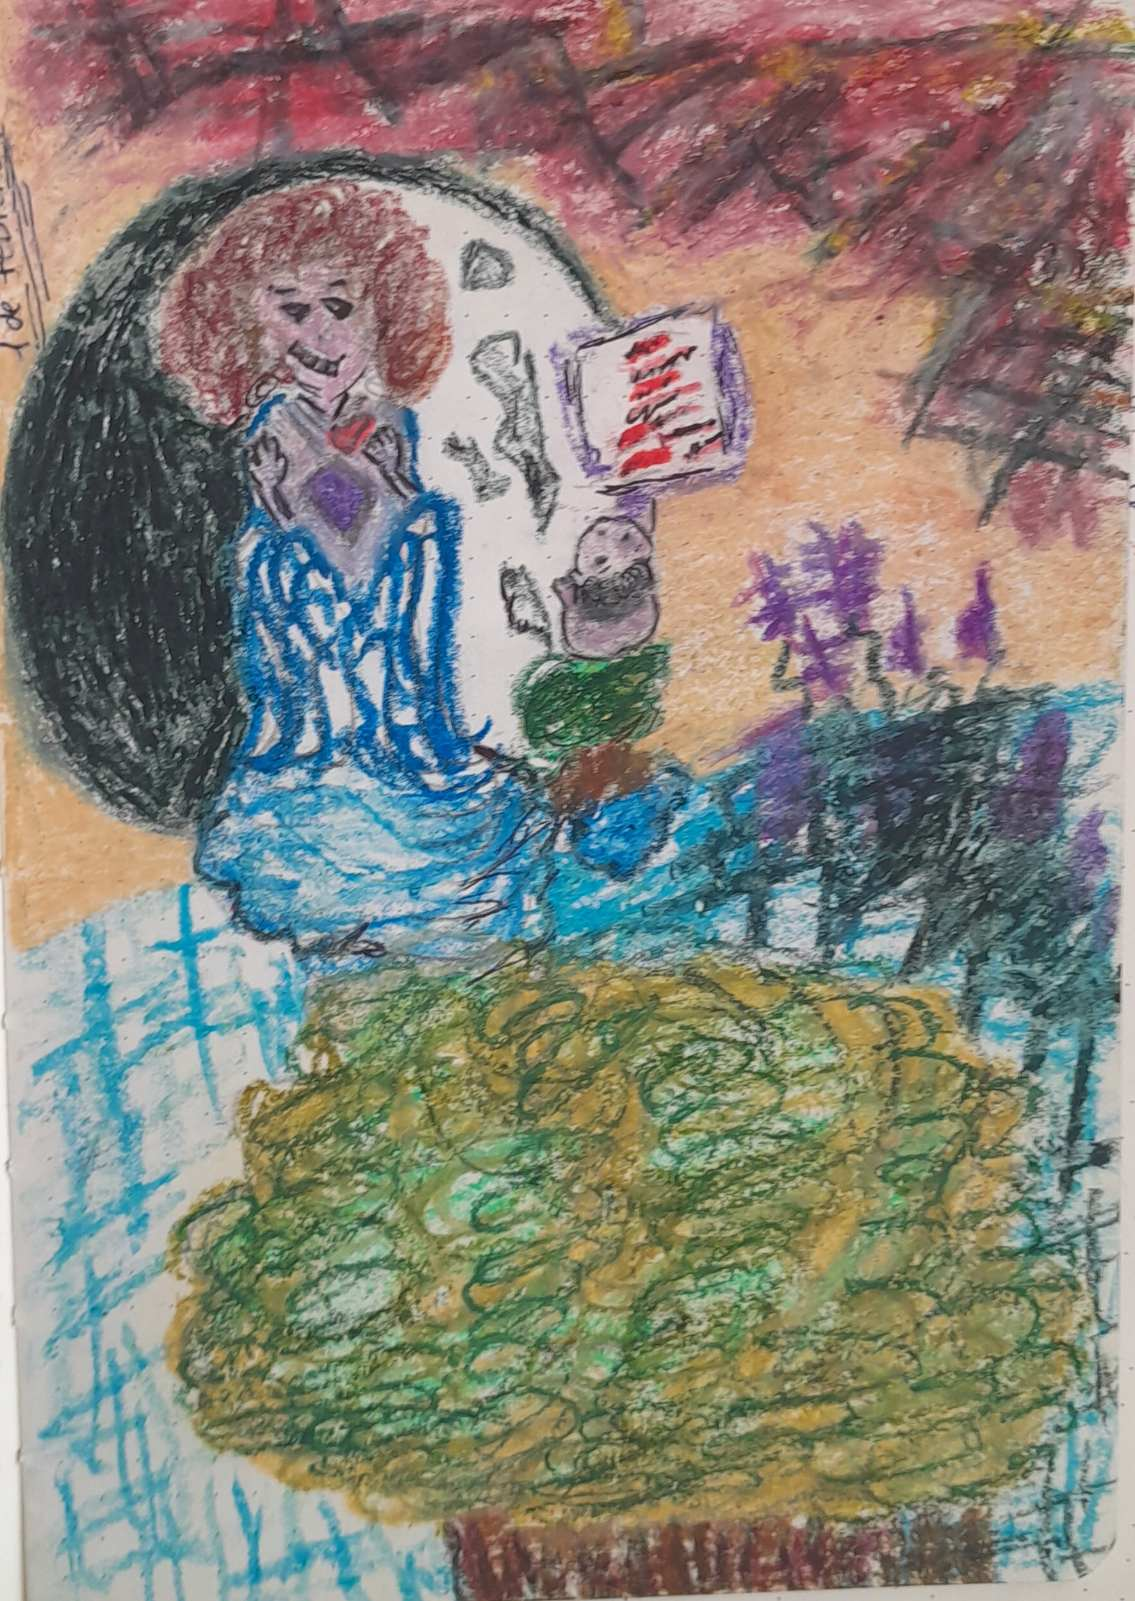
\includegraphics[width=\textwidth]{./images/1f81324dd8aaa9.jpg}
\end{figure}

% Digo en voz alta Gracias..
% Gracias por humillarme para que hoy pueda abrazarme,
% Gracias por cubrirme en tu útero tan deprimida, para transformar en compasión maldecir a otra vida.
% Gracias por reprimir mis emociones para que pueda tener un huracán de ellas y convertirlas en canciones
% Por romper ese cuento que de niña escribía para que la frustración cree algo más completo
% Gracias por querer ser de ti tan diferente que pueda ver tan claro el parecido
% Gracias por maltratar a mi padre para poder glorificar la figura de mi animus
% Gracias por nunca decirme que estabas orgullosa de mi, así pude resarle a la gran Madre para que me salve
% Gracias por con mi abuela compararme así puedo sentir que quedarme sola no será en mi una variante
% Gracias por hacerme sentir que soy una inútil así encarno el personaje del que nada tiene para perder
% Gracias por separarme de mi hermana, así he aprendido la rivalidad no deseada
% Gracias por hacerme sentir tanto enojo para en que en una úlcera pueda ser curada
% Gracias por hacer que quiera de la realidad evadirme  así pude refurgiarme en el arte
% De tantas otras partes que puedo agradecer, reconocer el dolor de otras mujeres hoy puedo compreder
% Gracias por que tanto he cantado lo que no pudo ser contado.
% Gracias por tu insatisfacción con la vida, así reinvento la mia con aventuras desconocidas
% Gracias por hacerte odiar y gritarte así hago frente a mi sombra antes que ella pueda tomarme
% Gracias  por mi sensibilidad, y el coraje de buscar de todo eso alejarme,
% Encontrar en otros hogares el calor de una madre
% Por en mi interior  sentir un vacío tan profundo que  se convirtió en espiritualidad
% Por querer torcer mi camino recorrido, así puedo detenerme a valorar.
% Espero algún día tu también puedas ver el aporte en mi vida que has realizado y nos abracemos sin juzgarnos.
% Para jugar muchas veces más a las muñecas, crear historias de príncipes y princesas
% Poner tu mano en mi cachete de las mejores caricias que se sienten

\begin{figure}[H]
	\centering
	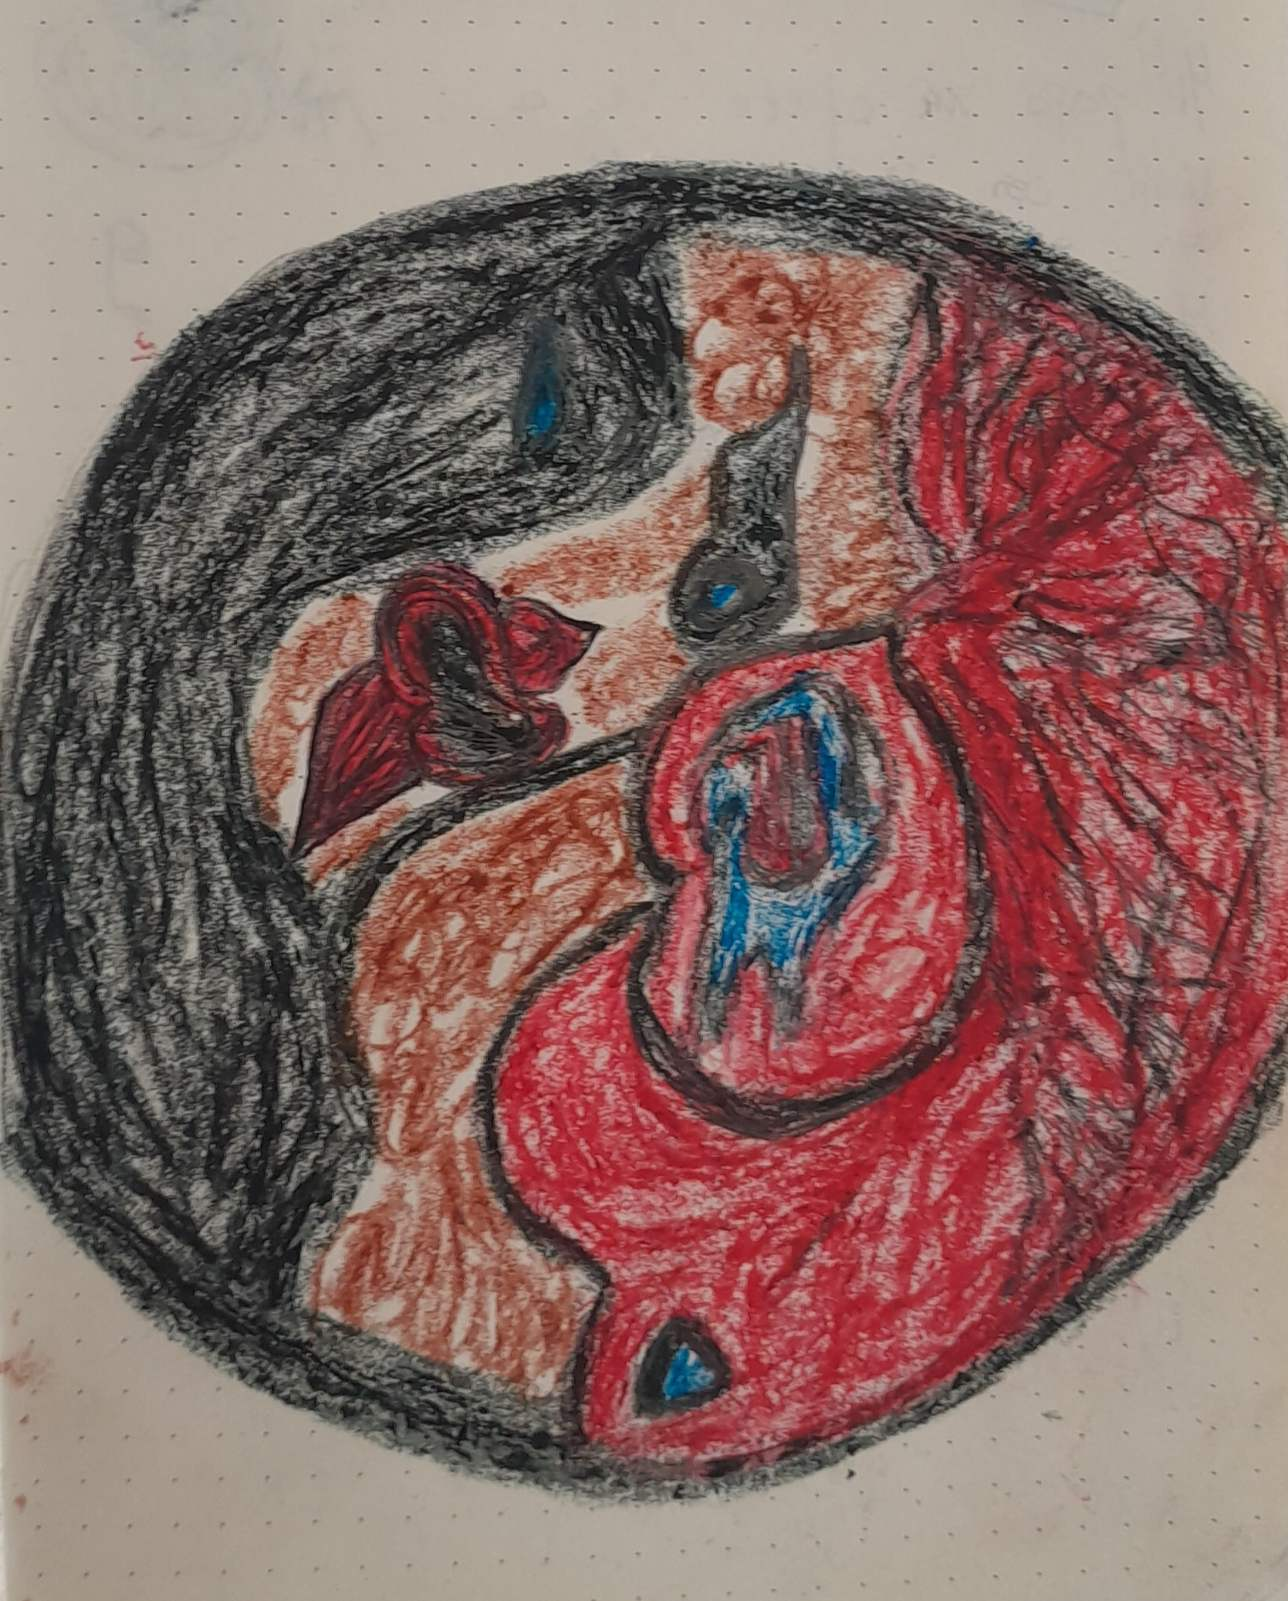
\includegraphics[width=\textwidth]{./images/1f81324dd84b67.jpg}
\end{figure}

\clearpage

\noindent\textbf{Las mujeres que habitaron}\\
Estoy enojada, me hierve la sangre, del caldo que aflora se vierte la olla, se caen los trozos de tripas humanas, burbujea espeso y caliente como el infierno, va quemando todo lo que en el camino toca.
Yo no lo prepare y eso me molesta, estaba así armado, con diferentes ingredientes fue elaborado, lo llenaban de odio, de envidia, de malas noticias, un poco de depresiones otro poco de desconformismo, lo agitaban como si danzara, y a su alrededor giraban vivoras escupiendo el veneno, y mientras la masa se amasaba con manos pegadas, golpeadas, maltratadas, la iban insultando, disfrutando, disfrutando, no le daban ninguna forma no querían practicar el arte,solo querían más y más escupir.
Se bañaban en la desgracia y así la fueron llamando vida.
Se regocijan en el caos y así aplaudían la estupidez con bandera de asañas, como jinetes de esos que cabalgan arañas. Pisando todo a su paso, confundiendo oro con gusanos, erguidas en la hipocresía, simulando libertades vacías, de pobres damicelas sin alma, sin nobleza.
Me invade en el vientre y repugna el olor, he bebido ese caldo sin ninguna opción, se manifiesta en mi como protestas sin intervención, fracasos, llantos, amores creados, con sentidos de castigo por vivir lo que soy.
Estoy enojada, no hay nada que valga de autocuracion, necesito que por si solo explote y no me acose, que vuelva a la olla, que lo traguen las otras y yo elija presenciarlo.
Decir que vengo de otro pueblo y no conozco ese olor, que de donde vengo tejemos y cocinamos amor, que ni siquiera soy capaz con mi imaginación audaz de vivenciar tanta maldad, no la escuché, no la respire, no la consumí ni me obligaron, ojalá pudiera decir que esas vivoras son para mi extrañas y que jamás a sus ojos he mirado, ni de su útero me he alimentado, así tendria mi útero entero y sano, así me hubiera engendrado de mi propio útero, el cual me alimenta de esperanza, de mensajes bonitos, de agradecimiento, y la sangre hubiese sido un nutriente para convertirse luego cada mes en una elección y pueda brindar por ser mujer, ni perfecta ni sobrehumana simplemente reconociendo la riqueza del dar y recibir, como un hermoso árbol, firme y constante, sin ver las manos del que quería talarlo, y respirando el aire, sentir como fluye en mi la sabía, que sube y  baja y me alimenta de limpia vida.

\begin{figure}[H]
	\centering
	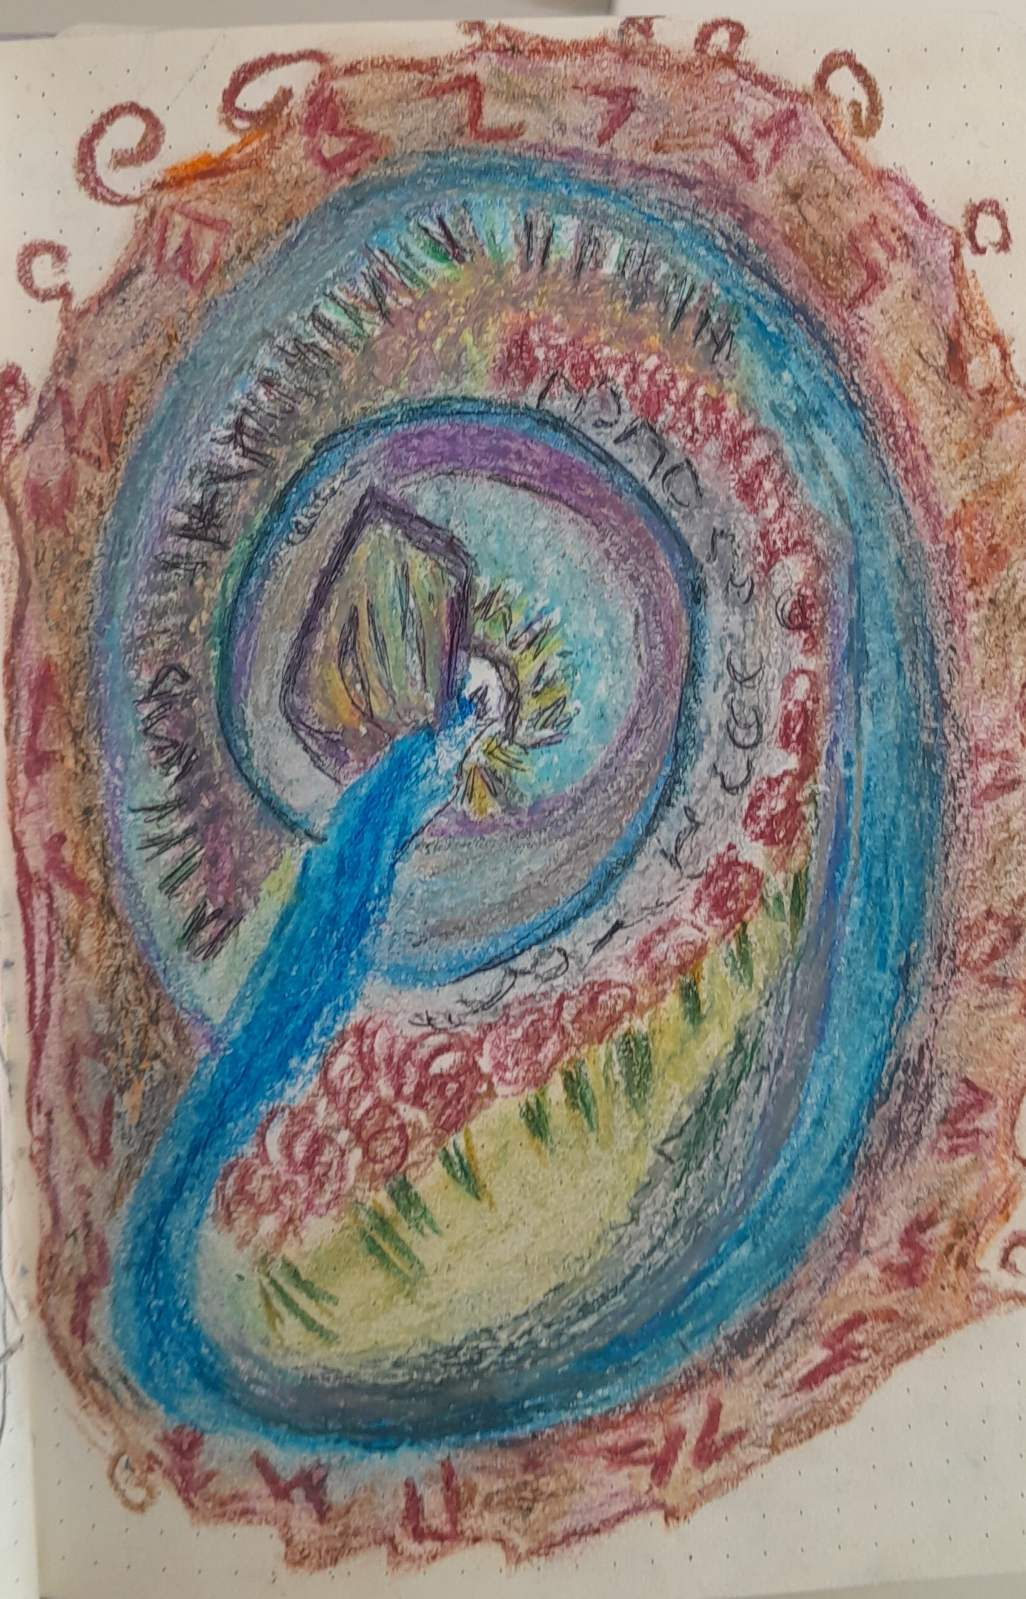
\includegraphics[width=\textwidth]{./images/1f81324dd8b935.jpg}
\end{figure}

\noindent\textbf{Redime a tu madre...}\\
La mujer que llora, por no curar las penas que la atormentaban  por horas.\\
La mujer que fue niña con ejemplos errados, que la formó extraña para entender su alma.\\
La mujer que de adulta no se llamo a su encuentro.\\
La que se hizo madre abriendo la puerta sin permisos ni certezas y volcó en su hijo el hilo que había olvidado.\\
Esa mujer herida que manipulo la vida, tocando oscuridades que fueron disimuladas...pero que en la superficie de la inconsciencia, ahi es donde estallan.\\
Elije el arquetipo de Madre que no tuviste, reconoce su rostro de blanca inmaculada, esa que todo cura y nos brinda el nacimiento...el segundo! aquel que viene de lo eterno, desde adentro.\\
Resguarda con abrazos la herida del pasado, un complejo viviente...sólo míralo y atiende,\\
Como brisa fresca reflejandose en tus manos...\\
Acuna la niña que no se sintió abrazada, como olas que irrumpen siendo partes del agua.\\
Ayrevete  a no ser  una gota perdida, a sumergirte y entregarte al misterio.\\
Porque en todo arte hay madres y madre dadora de vida hay una sola y justo y sin coincidencias es ELLA la que se encuentra la que abrió la fontanela, no la encontrarás en el  útero que te envolvio, sino como  la que en espiral siempre te acompañó.\\
Redime a la madre en tu interior, de humana a sabia, de incomprendida a alabada.\\

\clearpage

\noindent\textbf{Resignifica a tu madre}\\
Resignifica a tu madre,\\
Cambia su imagen por aquella que te cuida, que sólida en su esencia permanece.\\
La que te abraza con su equilibrio, te alimenta con su satisfacción.\\
Te inspira con su rostro iluminado y decora tu vida con los colores de su vestimenta.\\
La que te habla con opuestos, para que te descubras adentro\\
La que te sacude como un trueno y calma con agua bendita tu sed.\\
Cambiala por la que se sostiene en una flor y con su fragancia te lleva a confiar en ti\\
La que pone su mano en tu corazón y te renueva cada día con su amor\\
Esa madre que te guía sin juzgarte por qué bien sabe lo que puedes llegar a ser\\
La que expande y el veneno te extrae\\
Cambia una madre por otra, ahora que puedes hacerlo\\
A esa niña que no halló consuelo que se deje identificar por la madre que ha descubierto\\
La Madre eterna que con la brisa de su aliento limpia años de recuerdos y la sumerge en un nuevo nacimiento.\\

\clearpage

\noindent\textbf{Vuelve a casa}\\
Que no se trata de lo que digas, hagas, muestres, leas...que sólo se trata de una toma de conciencia, y que no se confunda con la bendita ciencia, se trata de ti, de tu propia esencia, porque no encuentra quién no sabe que anda buscando y tampoco aquel que en "collages" se anda mareando. No es "vivo el momento, como me apetezca", es pura impaciencia la que va comandado y crea y des crea según la marea, para el que está muerto sirve identificarse en cadenas, un vaso de antojos y otro de soberbia, mezclada con frases de autosuficiencia y de las de ayuda llamadas coraje, con tanta ceguera que encierra una era, se sabe el culpable y no quién lo vela, porque es más difícil mirar nuestra hoguera, mejor confundirse y pagar las deudas, de haber alejado los pies de la tierra. Y  donde antepasados estaban sembrando, hoy nos toca volver y auto abrazarnos, con tanta fachada y la casa está en quiebra, mejor sería  postrarnos y entrar por la puerta, esa puerta pequeña que siempre está abierta, que quiere acercarnos a nuestra inocencia,esa que veneramos y tanto anhela, que vuelvas a casa, que adentro es el verdadero afuera.

\begin{figure}[H]
	\centering
	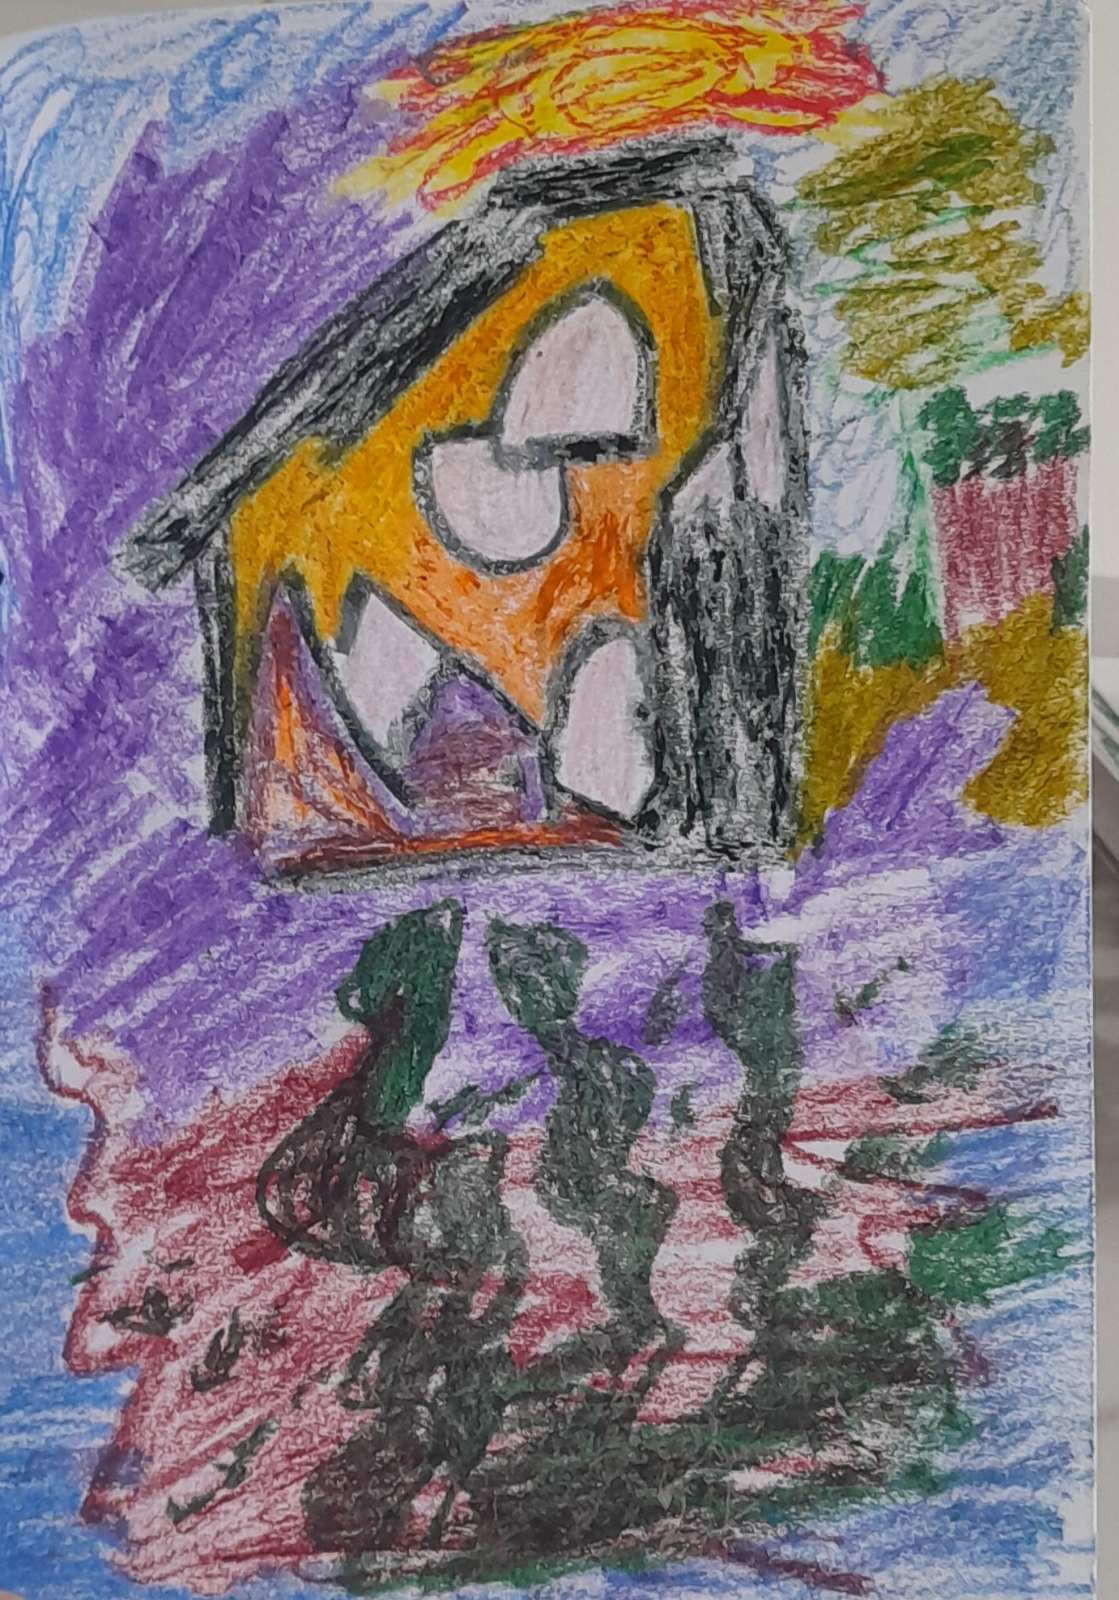
\includegraphics[width=\textwidth]{./images/1f81324df38bf5.jpg}
\end{figure}
%
% Chapter 3
\chapter{Sostenme Padre, sostenme}

\begin{figure}[H]
	\centering
	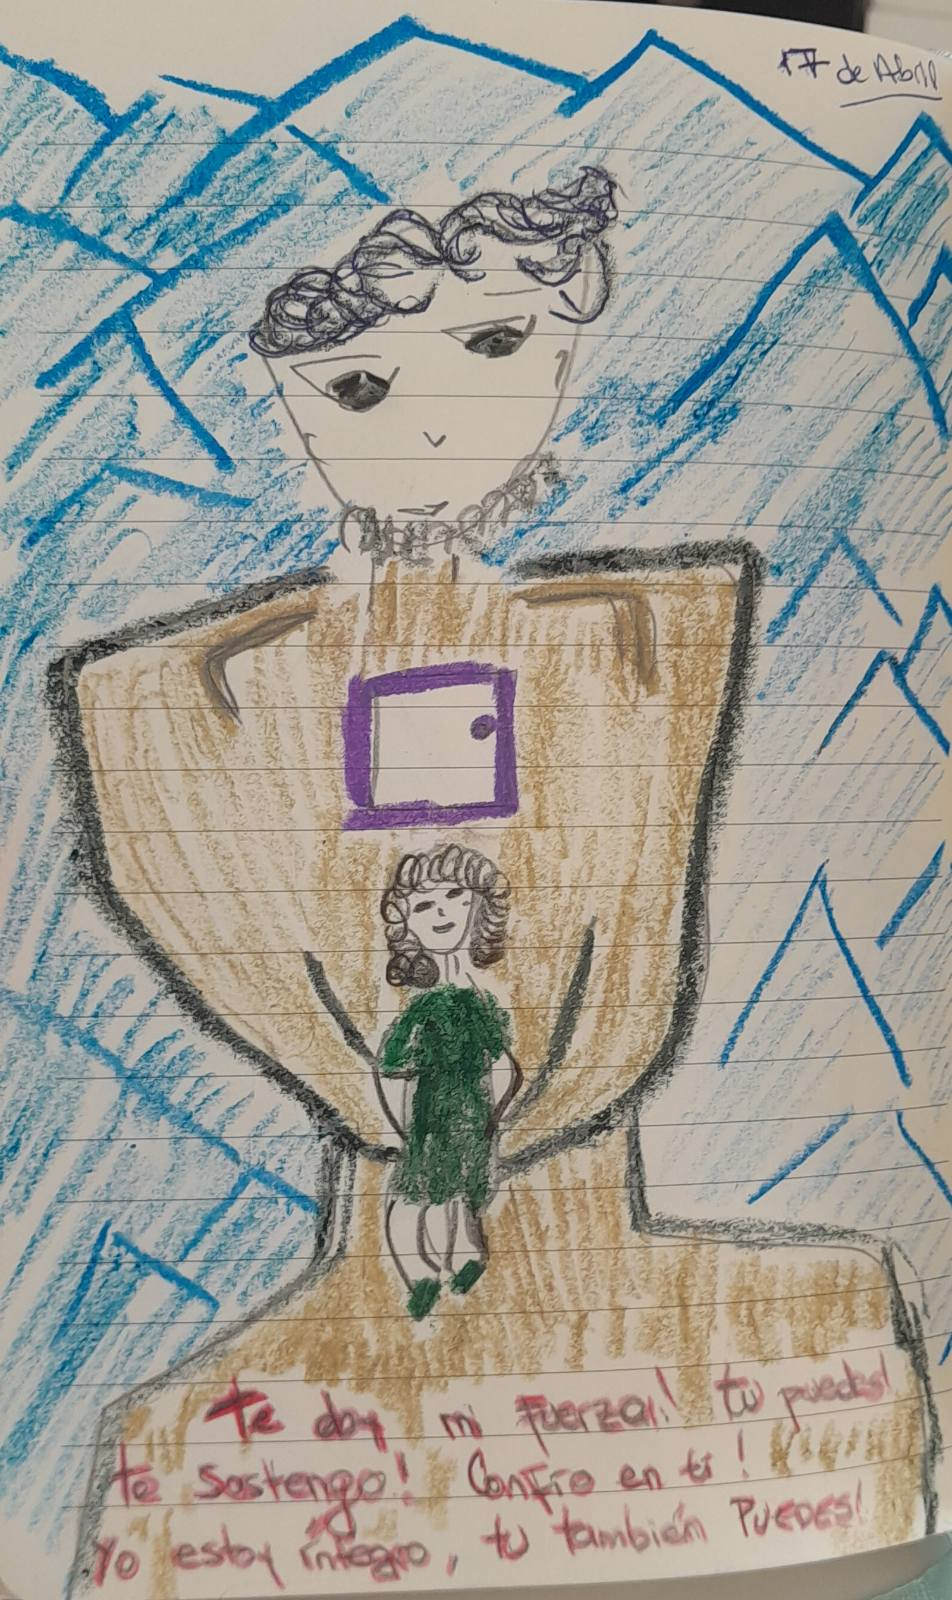
\includegraphics[scale=0.3]{./images/1f81324dd896f4.jpg}
\end{figure}

\noindent\textbf{Despertando}\\
Hoy vuelvo a morir, de a poquito, en trocitos, a un proceso que no domino.
Algunas muertes hacen mucho peso, reaparecen en espejos, en intentos,
Se aferran y me confunden...y si esa añoranza es hacia una pena?
La pena de lo que ya no soy, la pena de lo que ya no seré, la pena que hoy doy.
Me pregunto si no hay vuelta atrás y acaso en otro intento estaré extrañando a ese ser que se presenta como un extraño.
Se que adentro mío algo se ha despertado, como la luna que puede reflejar su luz en un mar calmo...
Contemplo esos momentos también extraños donde no me preocupo si algo se rompe, tan responsable de eso no puedo ser...quisiendo congelar el tiempo  y pudiendo manipular que no se rompiera, pero si se rompe que pasaría si lo tiro y listo?
Me silencio preguntándome cuando acepte que pudiera manipular la paz  de mi hogar de la niñez
Cuándo comencé a beber las palabras de si eso sucede es porque...
Van muriendo esos recuerdos y renacen diferentes,  como la abuela que incapacitada camina en mis sueños ya no fundida en su cama, aunque su aliento no la acompaña en esa vida no vivida, en esa llama no encendida.
Y quiere cobrar vida en mi cuerpo, atormentando mis oídos por lo que escuchaba, con la soledad de una abuela siempre comparada, que se sostenía como un manifiesto maléfico.
Quién diría que no hay una edad para morir, y que el segundo nacimiento no estaría velando un despertar eterno?

\begin{figure}[H]
	\centering
	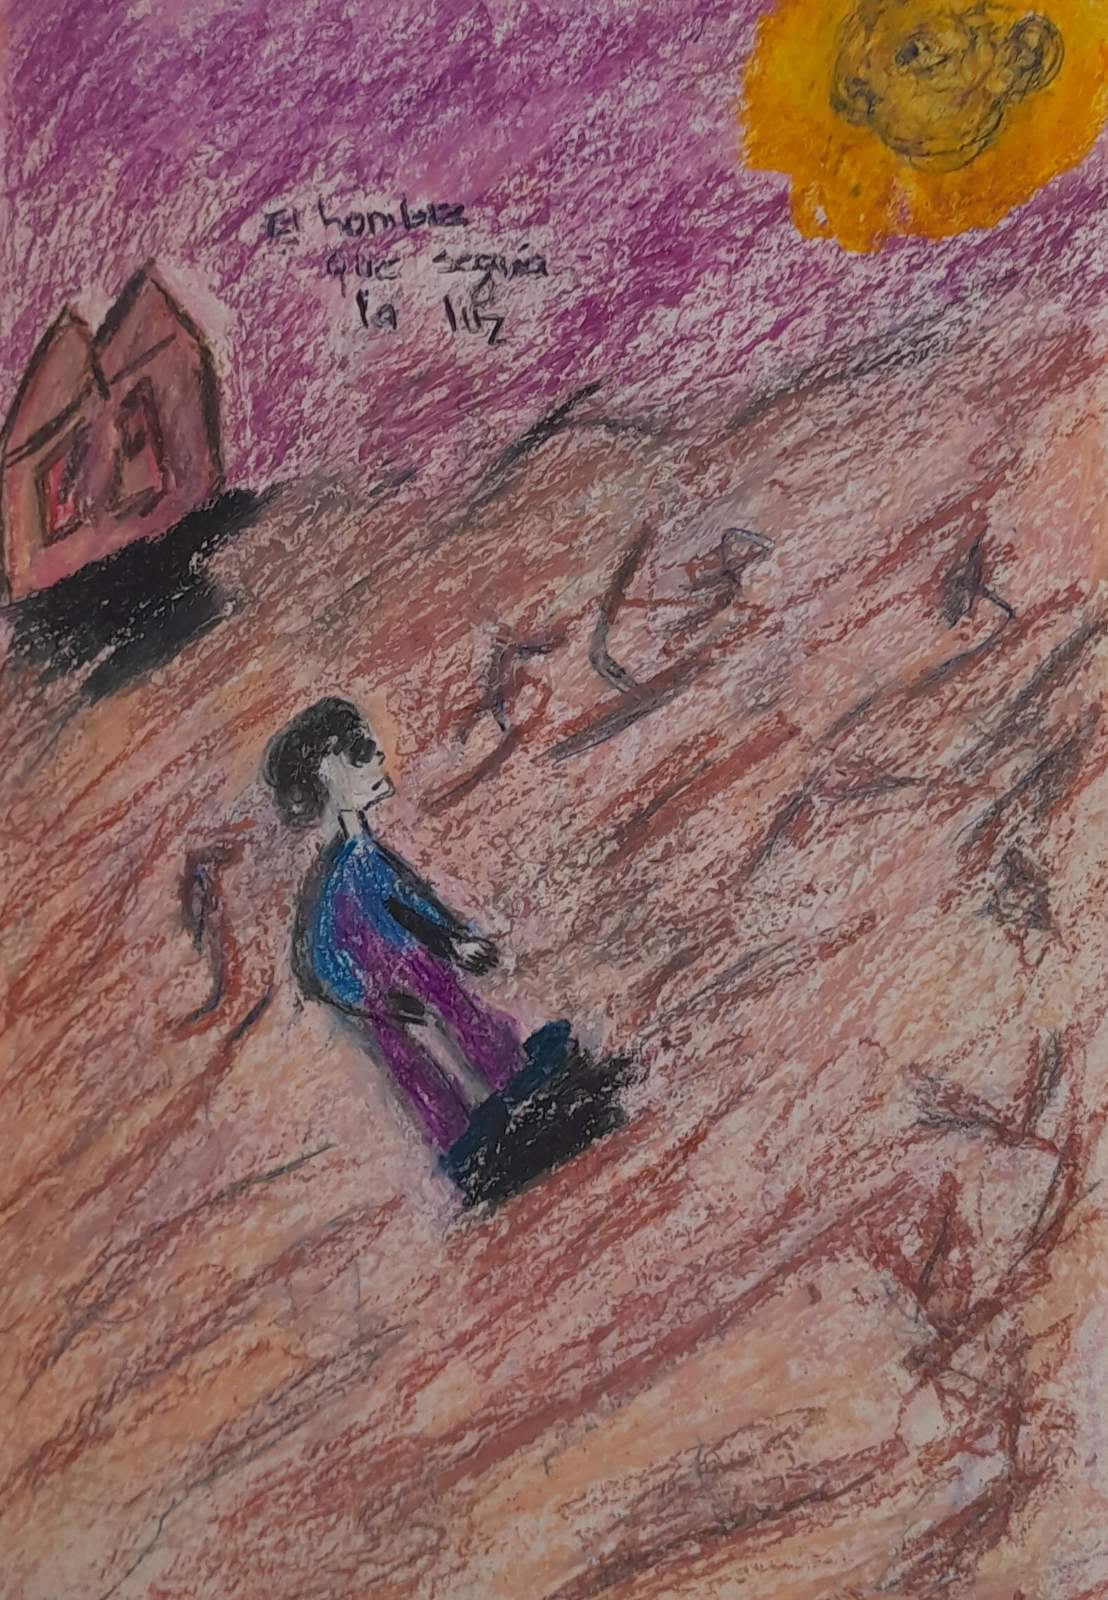
\includegraphics[width=\textwidth]{./images/1f81324dd99091.jpg}
\end{figure}

\clearpage

\noindent\textbf{El hombre que seguía la luz}\\
Felipe, el joven Felipe, conocido por pocos como Philip, o el filipino, de tez transparente y ojos grandes, con arrugas en su mueca de sonrisa torcida.
Tranquilo, siempre con su andar lento, pocas palabras y acertadas frases de aliento.
Queridos por aquellos que vivieron con él algún encuentro.
Ya hacía mucho no se lo veía en el pueblo, era lo que esclamaban sus vecinos de Nordesto.
Sin embargo Felipe se encontraba más presente que nunca, viviendo con interés sus nuevas aventuras, no le desagradaba tanto mudarse cada dos años, o a veces de forma inesperada, según cómo ella se presentaba.
Si bien le costaba adaptarse a los habitantes y conseguir el trabajo en el nuevo lugar, las oportunidades de un artesano como bien se sabe, están en sus manos.
Así iba encontrando que haceres para construir su morada, siempre con las ventanas hacia su inspiración.
Como desearía que alguien apreciara lo que mis ojos pueden ver anheló una tarde Philip, tal vez en el pueblo más cercano encuentre está vez un amigo para contárselo
El joven construía su casa siempre en las afueras de la ciudad, ahí se sentía más seguro y con tiempo para poder apreciarla.
Pasados unos meses, un señor de barba y uniforme blanco comenzaba a serle una voz confiable, casi que se veía tentado a invitarlo, pero luego le entraba de nuevo la desconfianza, en el fondo sabía que nadie le iba a creer.
Es hombre aparecía seguido por su trabajo, le preguntaba cómo se sentía hoy, y muchas veces lo escuchaba, le recordaba a él mismo hablando también sólo por las noches.
En cambio la señora abrazos, como Felipe la llamaba, venía cada madrugada y sin decir nada, solo lo saludaba con uno de esos abrazos que cuentan historias de musas y hadas.
Pero una tarde al volver a su casa, vio que la luz  se había alejado, era otra vez hora de tomar sus pertenencias y moverse de lugar, avanzando hacia el este, acercándose para no ver a la luz tenue.
Ese era su secreto!!!! Aún recuerda cuando la vió por primera vez, se presentó en su primer hogar, tan brillante y cálida que supo al instante que sólo se dedicaría a seguirla.
Claro que lo distraian sus actividades diarias, algunos días sumergido en sus fantasias, otros solo vagando en sus pensamientos.
Al emprender el camino para plantarse y contemplarla, notó que ella no se detenía como las veces pasadas, avanzaba sin fuerza y desaparecía.
Felipe angustiado y desesperado, armó su hogar ya cansado a mitad del bosque...
Esa misma  noche se apareció en sus sueños una niña, que con una vocesita angelical le decía:
Despierta papá, despierta!!!!!, no sigas la luz!
Con tu familia regresa!!!!!

\begin{figure}[H]
	\centering
	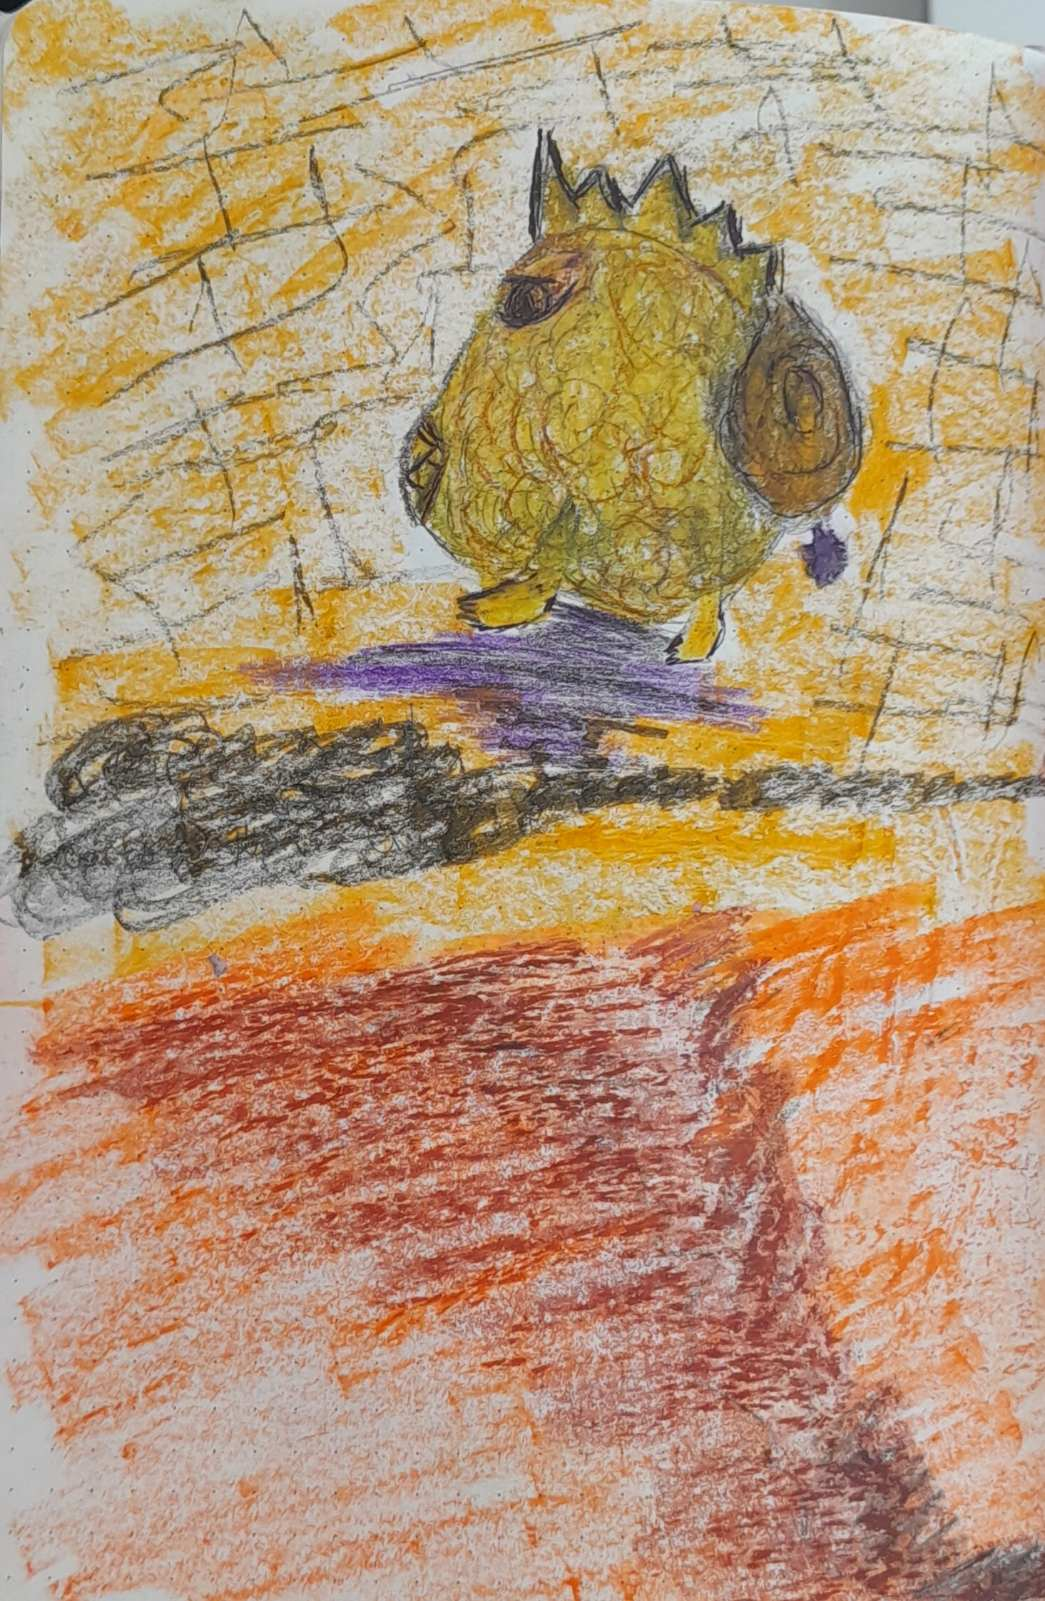
\includegraphics[width=\textwidth]{./images/1f81324ddf04ba.jpg}
\end{figure}

\noindent\textbf{Como aliados}\\
Quiero conocerme, no para encasillarme, sino para sostenerme...
Saldar con mis latidos los encuentros desconocidos.
Estar atenta quién entra, Cómo entra, como suena, en que lugar de mi se encuentra.
Si es por mis ojos, orejas, como proyecciones, vivencias...
Seguirle el rastro a la la mujer que es transparente y cubre a las que no quieren ser vistas, descubiertas, detectadas, para que no las moldeen ni interrumpan su morada.
Quiero reconocerme para cocerme donde duele, armar otro punto que me lleve a otro rumbo.
A esas almas que andan deambulando permitirles un escenario y con mi humilde yo se reacomode lo que es obra, lo que sobra, lo que decora y lo que estorba.
A los hombres que me visitan por las noches, me ha visitado el sabio! siento el haberte despertado, sin querer toque tus pies, pero que grato fue que me puedas ver.
Aunque en tus asuntos andabas tentado, te hiciste presente, no puedo ignorarlo.
Al enamorado, que tan hábil me impresiona y se retira a la mañana que asoma.
Al hombre fuerte, guerrero que me protege.
Quiero con todos estos personajes en diferentes momentos, en los cuales  toman cabida, darles vida y hablarles, escucharles, saber cuál es el que en un ronroneo me azota, me confunde, me decepciona, sentir cuando se cuelga en mi pecho y quiere ser tragado el amargo sabor de lo no logrado, de las aspiraciones fallidas, de esa vida no vivida.
A los que en silencio me velan, y  hacen caer todos los velos, invitandome a ir adentro, saben muy bien como anhelo y reverencio esos momentos. Mi propio ser, espíritu eterno que calma la sed.
Y aunque aparezcas a altas horas, tu solitario, tu que me asfixias y al mismo tiempo me hipnotizas con tus misterios añorados, teniendo discusiones con el que me aterriza y en una realidad  a la luz del día como un escorpión me atemorizas, me paralizas.
También estás invitada a este encuentro la que me absorbe toda la energía en apegos y deseos, en emociones enfermizas, lamentos, juzgadoras demandas que a mí y a otros castigan, la que a la cama bañada en llantos me devuelves hecha trizas.
La energía que da ímpetu y también la que me denigra, las vengo observando, hay de ustedes como pican.
Que vayan pasando por favor de a uno, en sintonía, así no me agarran desprevenida, después de todo soy yo la nodriza que elije como alimentarlos, aplaudirlos, sensurarlos, para que no sean tan extraños y caminemos juntos en el si mismo orbitando, codo a codo, como aliados!!!

\begin{figure}[H]
	\centering
	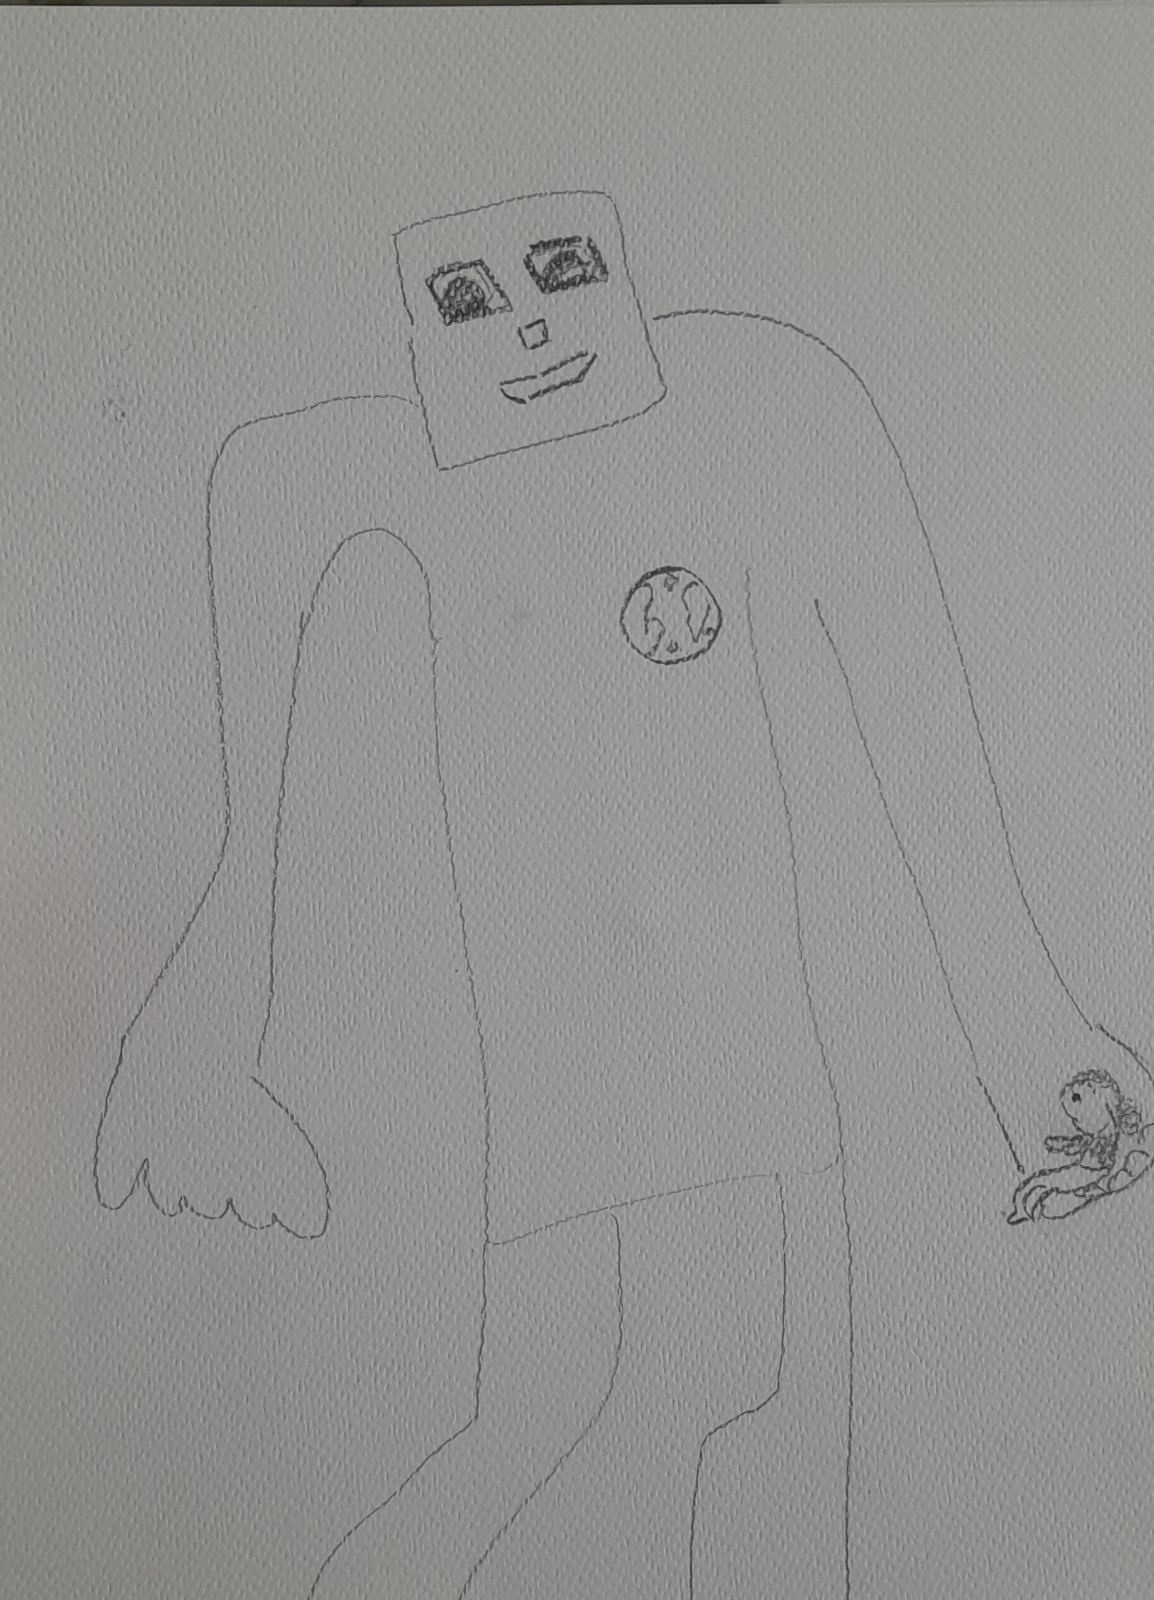
\includegraphics[width=\textwidth]{./images/1f81324df1ed85.jpg}
\end{figure}

\begin{figure}[H]
	\centering
	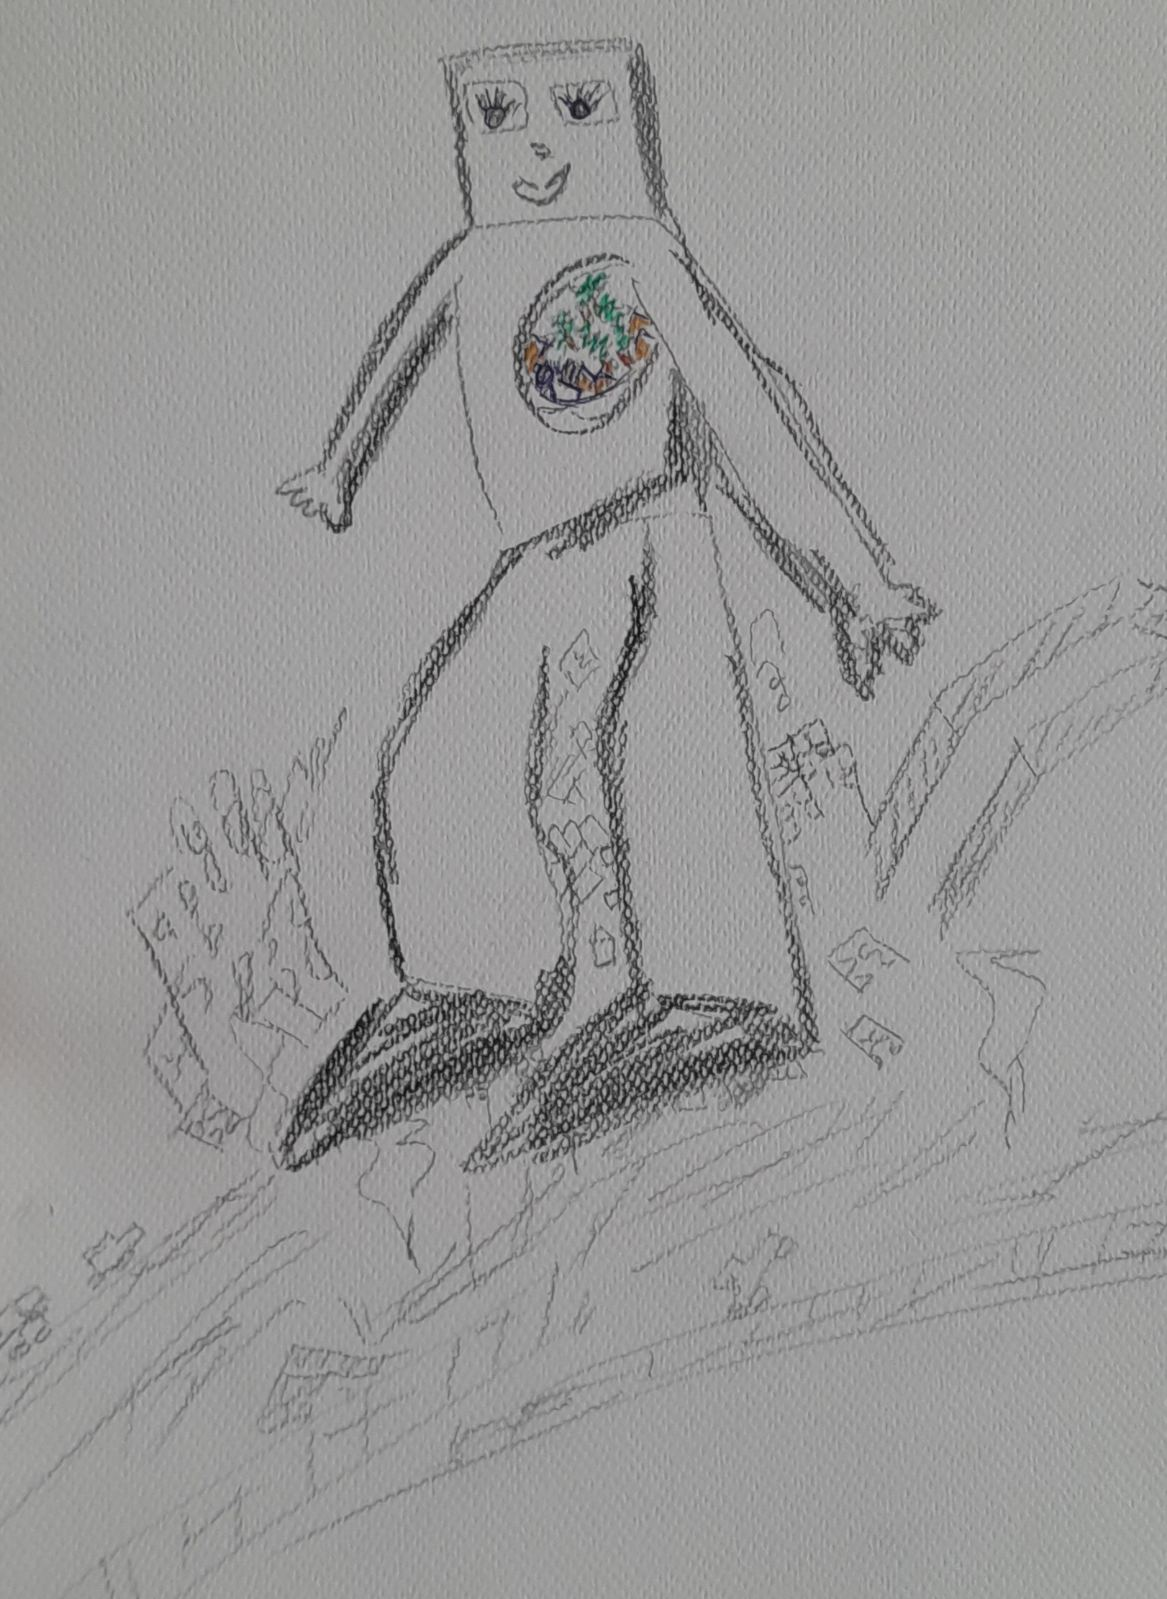
\includegraphics[width=\textwidth]{./images/1f81324df12268.jpg}
\end{figure}

\clearpage


\begin{figure}[H]
	\centering
	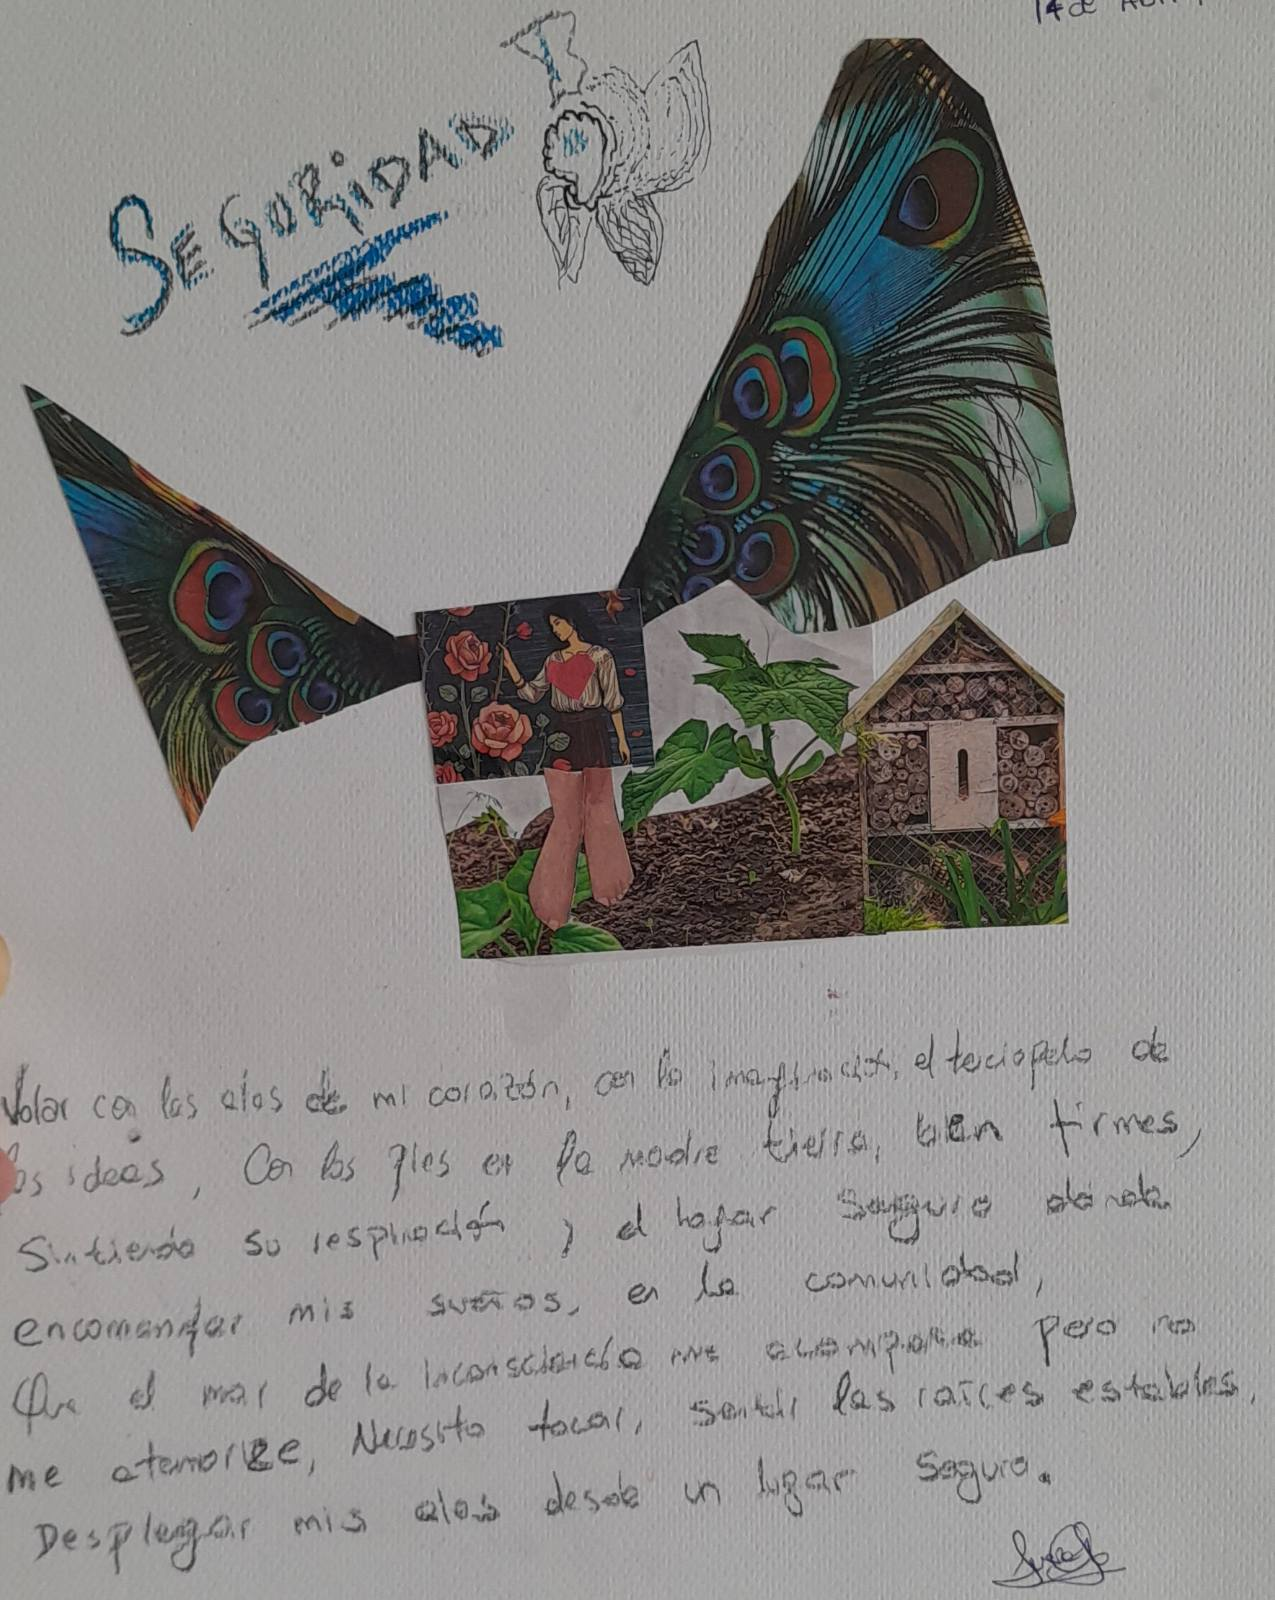
\includegraphics[width=\textwidth]{./images/1f81324df158d6.jpg}
\end{figure}

\clearpage

\noindent\textbf{Seguridad}\\
Gracias a mi animus amado, al hombre que me tomo fuerte de la mano, le dio importancia al sentir de mi cuerpo, manifestando mi personalidad que estaba entre lo que fui y lo que soy para construir juntos lo que será.
Ese enamorado que me visita por las noches, me devuelve el misterio, las ansias de aprender.
Al que me dio un empujón mostrándome mi valentía y valor.
El que me prometió un mundo donde habitar, y me protege.
Me ayudó a que la intuicón vuelva tomar forma para marcar que mi ser ya conocía de, dónde y hasta cuándo iba el verso.
Hoy celebro haber vuelto un poquito a mis tierras y guardar en esta reliquia lo valioso, respirar profundo en momentos de incertidumbre, querer cuidarme, querer cuidar, gracias por aparecer de forma material.
Y si bien muere el amor que adolesce le doy paso en mi vida al amor que sostiene.

% Chapter 4
\chapter{Simbolos de orientación}

\begin{figure}[H]
	\centering
	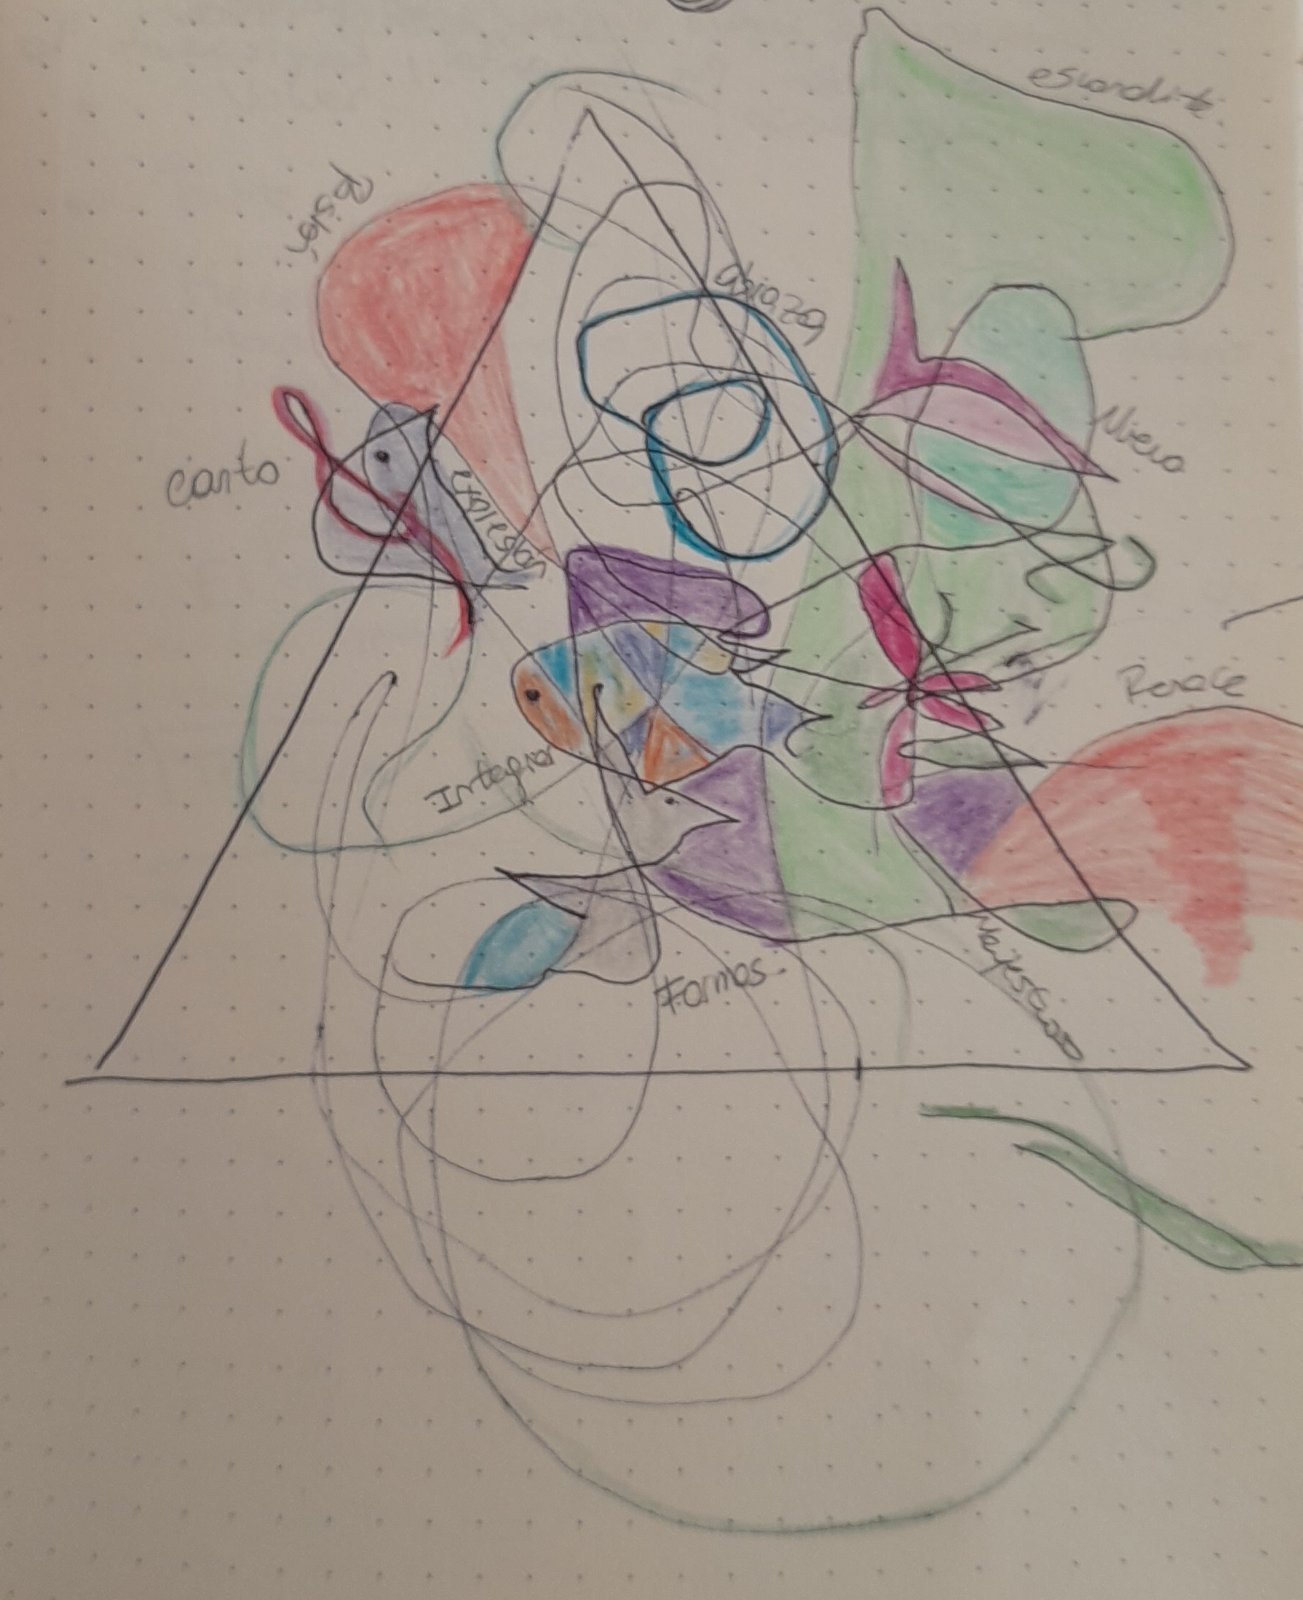
\includegraphics[width=\textwidth]{./images/1f81324dd960fe.jpg}
\end{figure}

\begin{figure}[H]
	\centering
	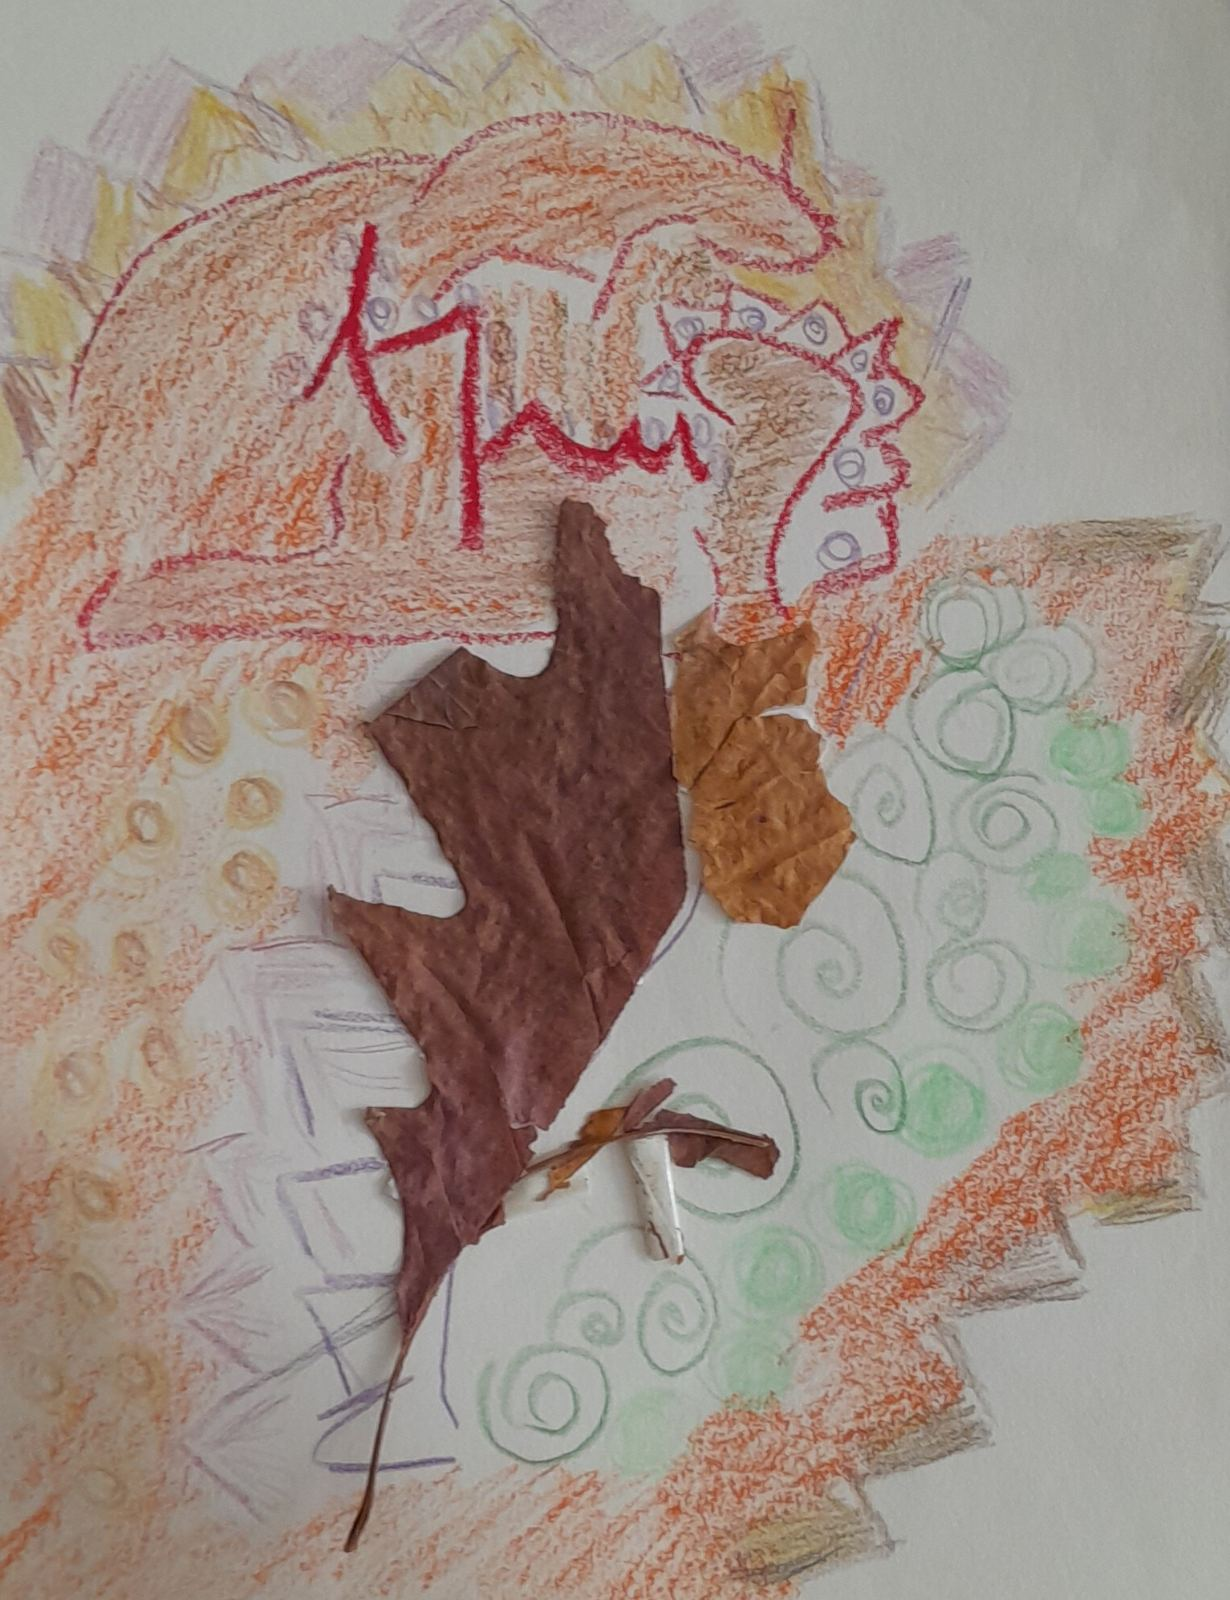
\includegraphics[width=\textwidth]{./images/1f81324df11e90.jpg}
\end{figure}

\begin{figure}[H]
	\centering
	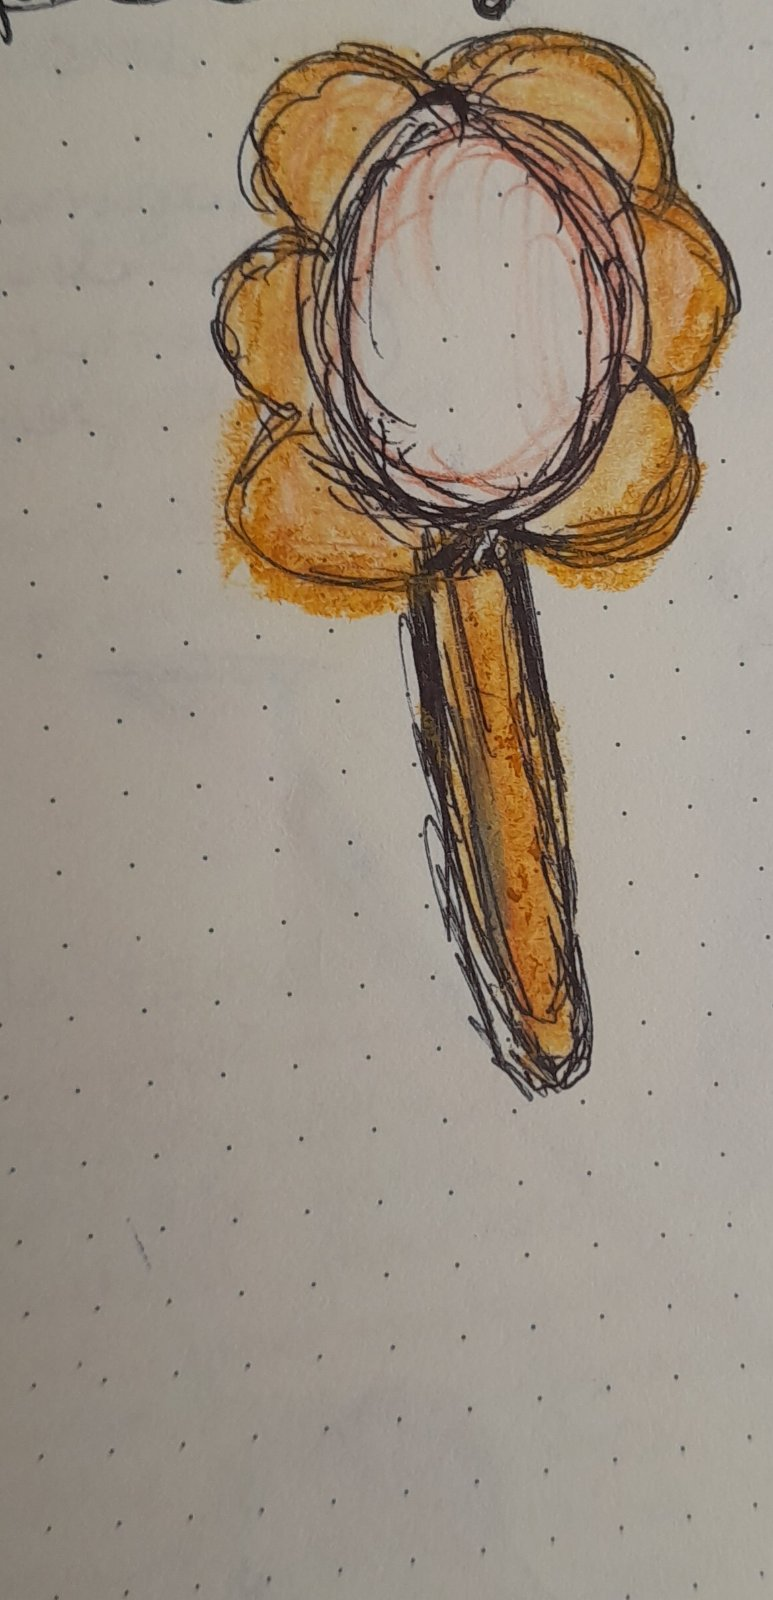
\includegraphics[width=\textwidth]{./images/1f81324ddf220c.jpg}
\end{figure}

\noindent\textbf{Proyección}\\
Soy el espejo que te esperaba, llegue al mar para que me puedas ver brillar, Sé que en las aguas de tu inconsciente puedes observar, oír, tocar.
En la deriva flotando me mantuve en la inmensidad, en el momento justo donde los rayos del sol entregaban su último reflejo, brille como oro puro.
Te acercaste a mí, deseando la riqueza, se que te atraeria mi forma antigua, ancestral una reliquia con la que fundes horas y ratos de vida consciente añorando vivir.
Cuando me tomaste en tus manos sentiste mi belleza y al volteame tu rostro fue el que se reflejó, con gestos de sorpresa y contemplación, nos conectamos al instante... Cuánto arte!
Me preguntaste cuál es mi mensaje, te respondí "mira en lo que te has convertido hoy"
Seguramente ni de aprobación ni de rechazo hayas escuchado el tono de mi voz.
Aparecí como un recuerdo de lo que fuiste y por lo que caminas hoy.
No pude responder a tu otra demanda, tal vez de ansiedad estaba cargada, más creo que sabes bien la respuesta.
Porque soy ese objeto, el que muestra la verdad, en las recetas con los ingredientes que vamos mezclando, cuando va al horno  quién puede asegurar el resultado?

\begin{figure}[H]
	\centering
	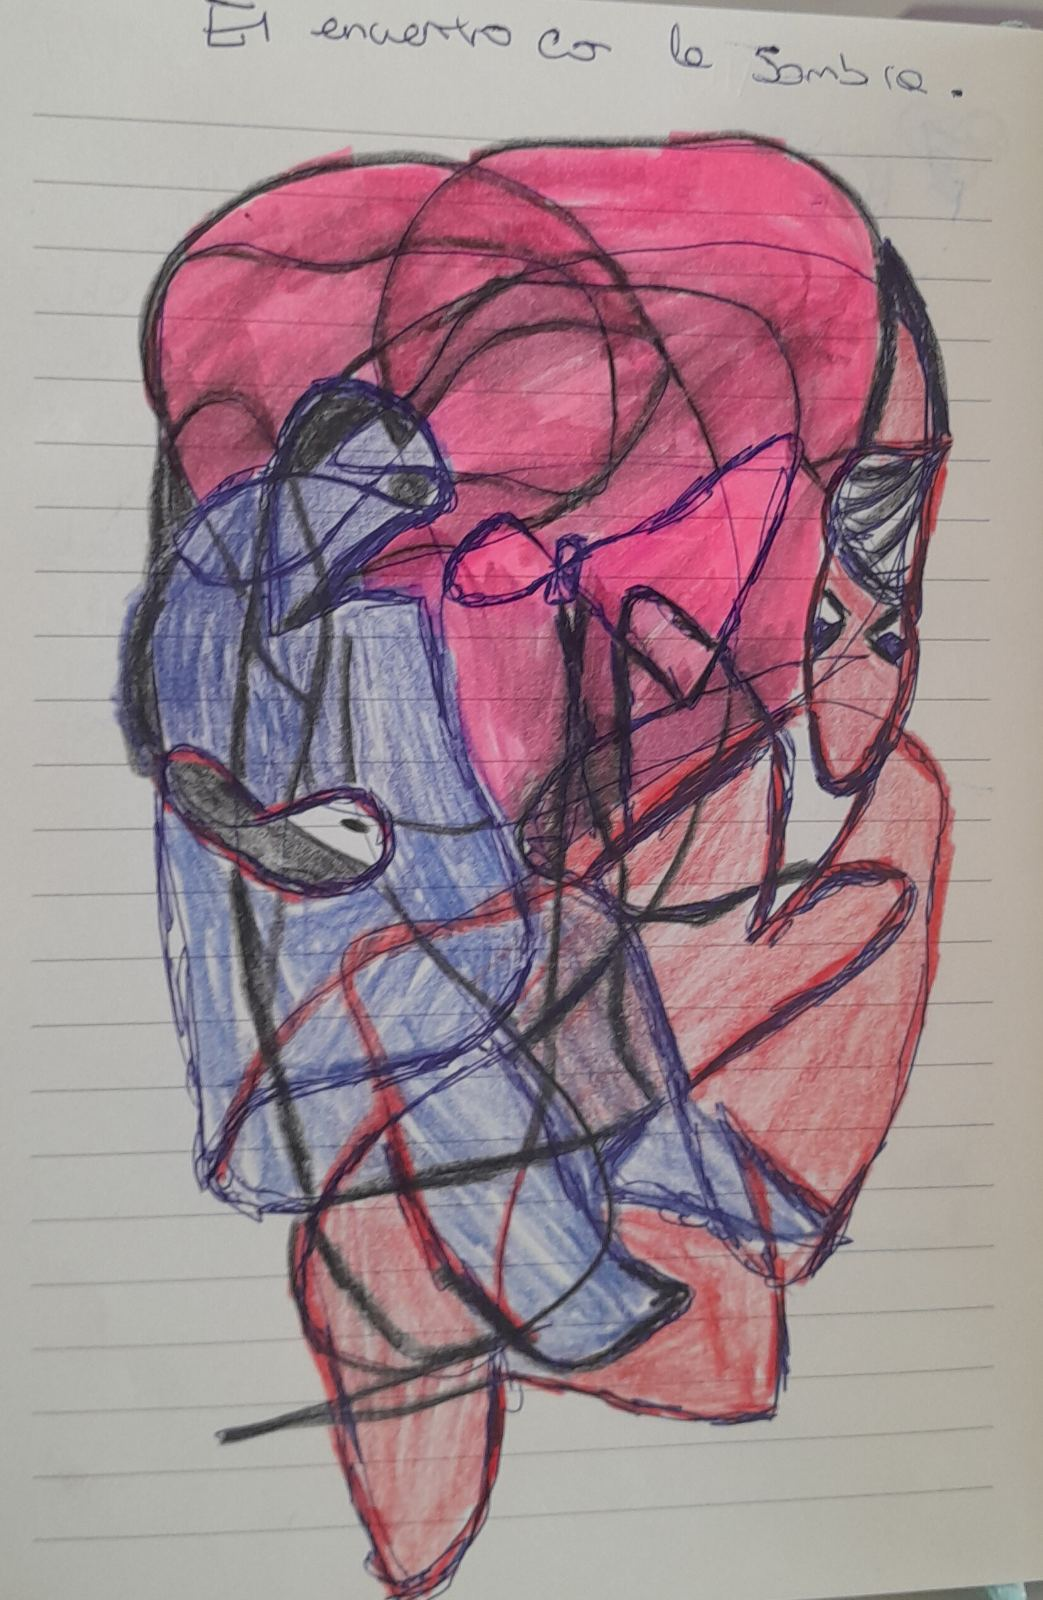
\includegraphics[width=\textwidth]{./images/1f81324df25232.jpg}
\end{figure}

\noindent\textbf{Sombra}\\
Y un dia llegue, tan elocuente, lo venia planeando, cómo me aparezco?, cómo sacudo su vida para que me atienda, me vea, me rescate, a la luz me vuelva?\\
Cuando todos duermen, llamare a su puerta, le mordere sus dedos para que lo sienta, le dire te odio para que me venza, como dadora de vida camuflare mi presencia, total ya no era bueno el lazo consciente con ella, sere repetitiva y constante, le dare escenarios llenos de opuestos, pondre varios personajes tramando  un encuentro.\\
Sere madre, padre, hermana, amores frescos, una amiga de infancia, todos aquellos que le despierten desconsuelo, sere tan intensa que amanecera sufriendo, deseando aquello, soportando inciertos, replanteando su dia como dos paralelos.\\
No cesare en mis intentos, aunque me convenza y se mantenga lejos.\\
Le dare motivos para rechazarme y seguir creyendo que todo es un cuento, pero hare hueco en la escencia primaria de lo que va muriendo.\\
Y si acaso me atiende estallara la tormenta y si tiene coraje no correra a la tienda, le dejare mensajes de duendes que la velan, para que se ate fuerte y viva la experiencia,\\
Algunos me llaman sombra, otros reminiscencia, pero si me aparezco no importa como me vean, estoy adentro tuyo, el que tiene ojos que vea.

\begin{figure}[H]
	\centering
	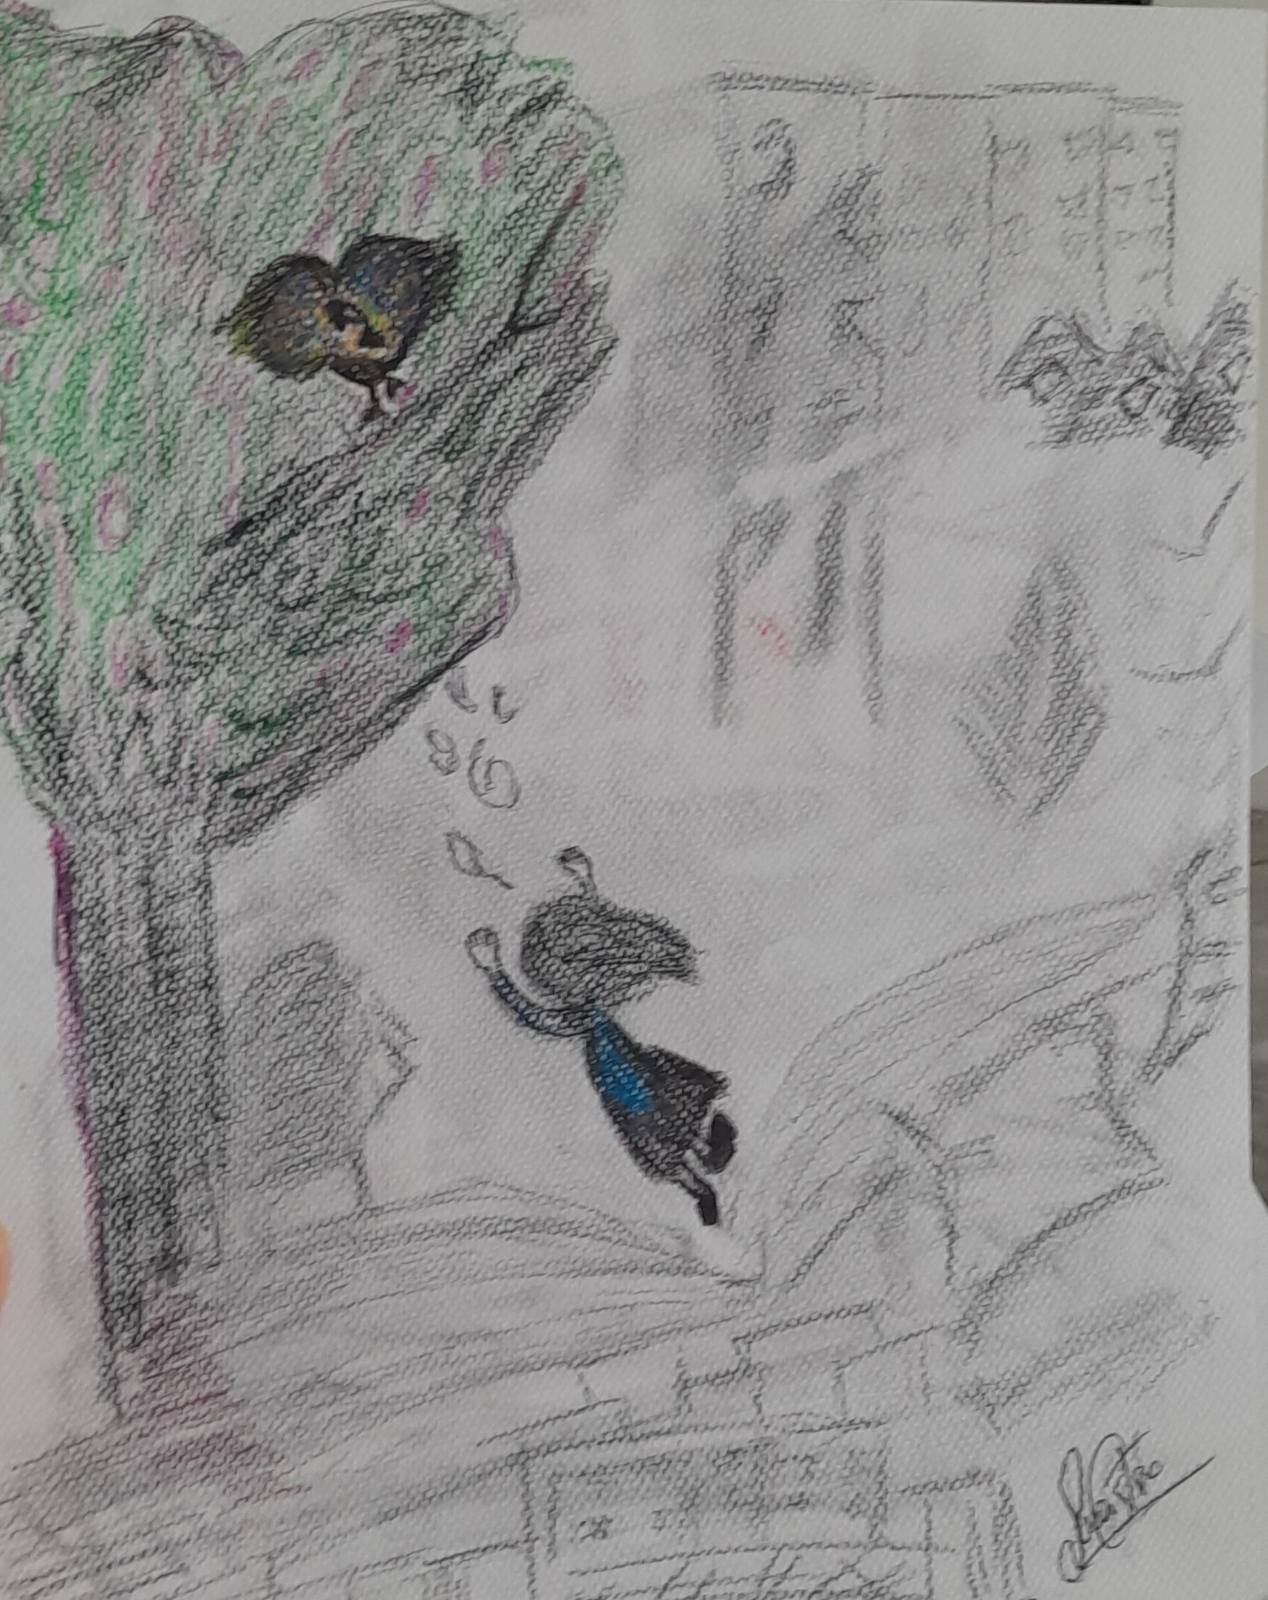
\includegraphics[width=\textwidth]{./images/1f81324df14aba.jpg}
\end{figure}


% Chapter 5
\chapter{Criaturas del arte}

\begin{figure}[H]
	\centering
	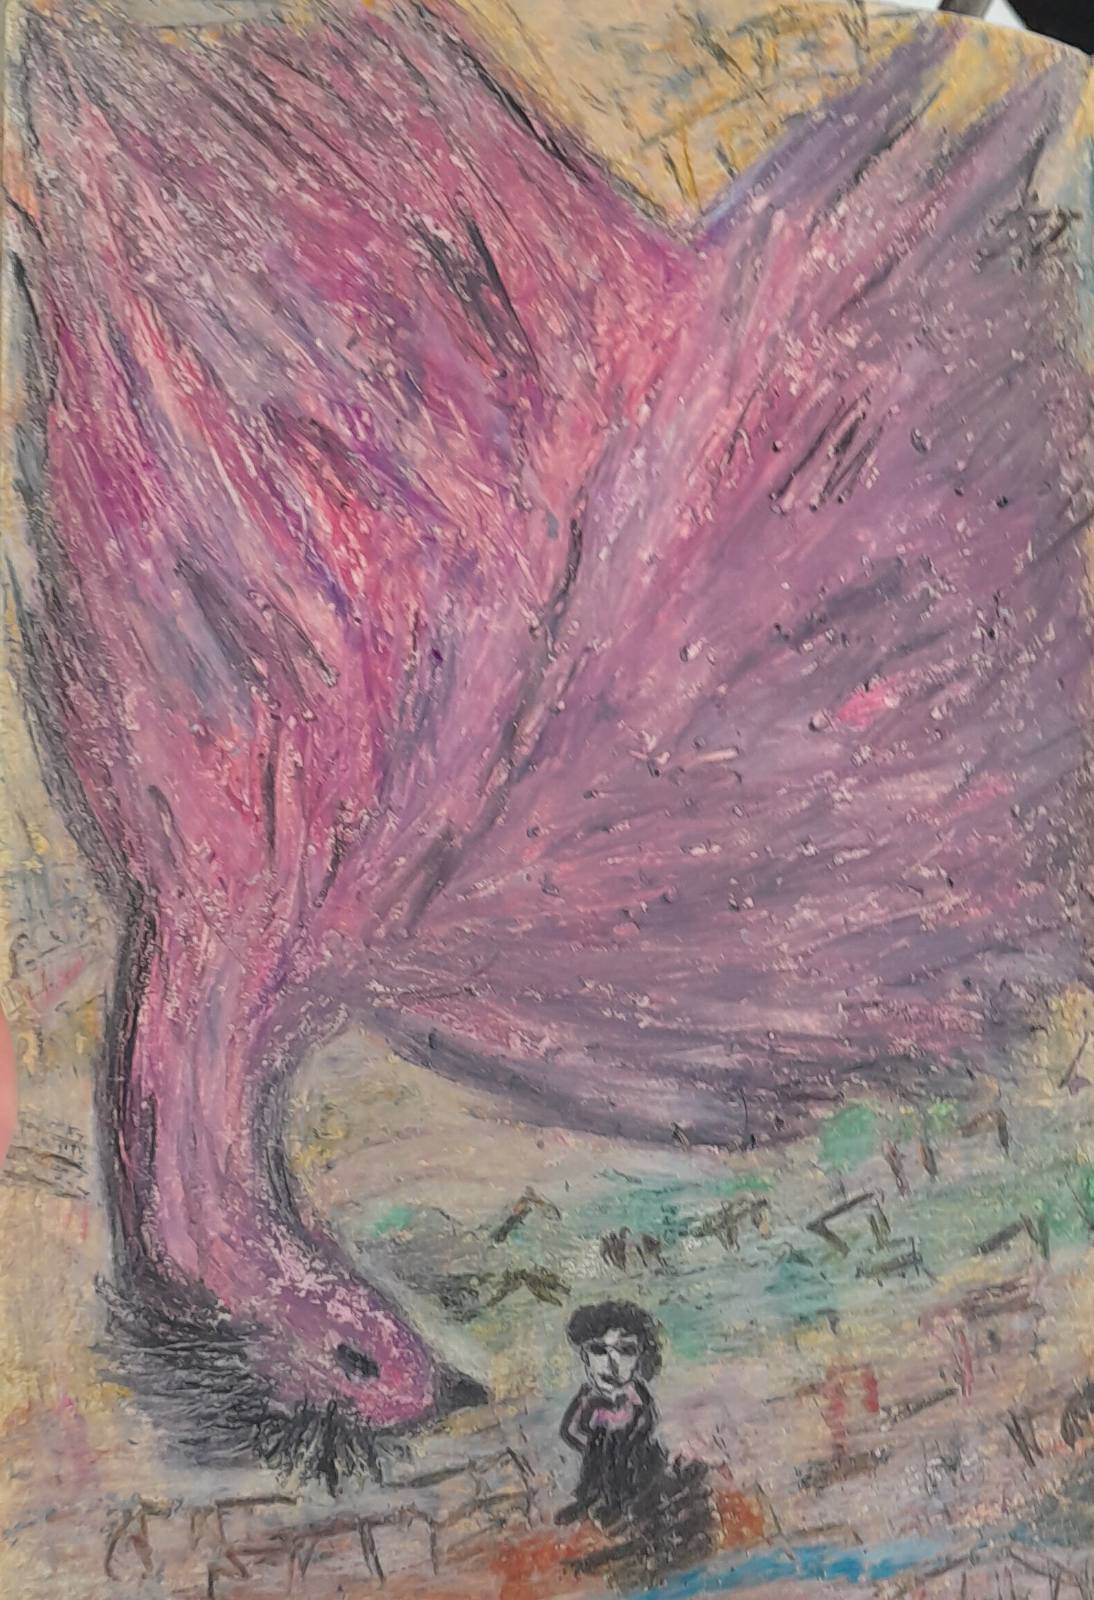
\includegraphics[scale=0.3]{./images/1f81324dd8eef5.jpg}
\end{figure}

\begin{figure}[H]
	\centering
	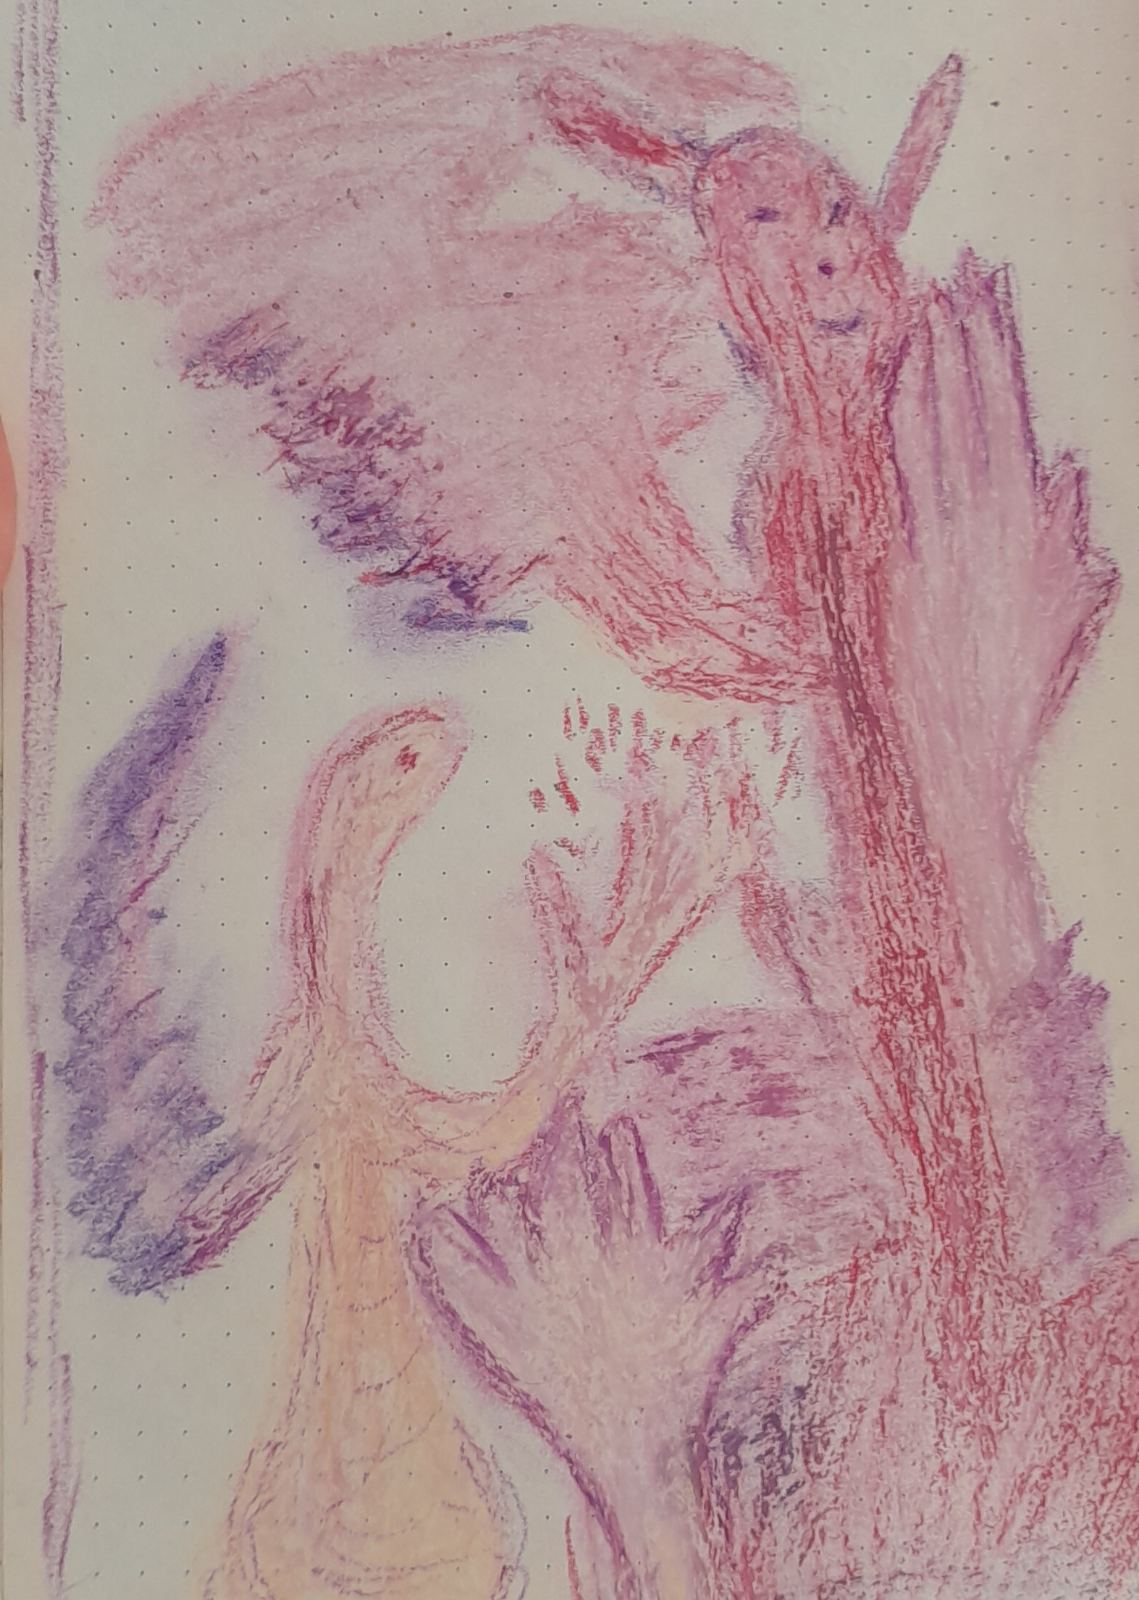
\includegraphics[width=\textwidth]{./images/1f81324ddf333e.jpg}
\end{figure}

\begin{figure}[H]
	\centering
	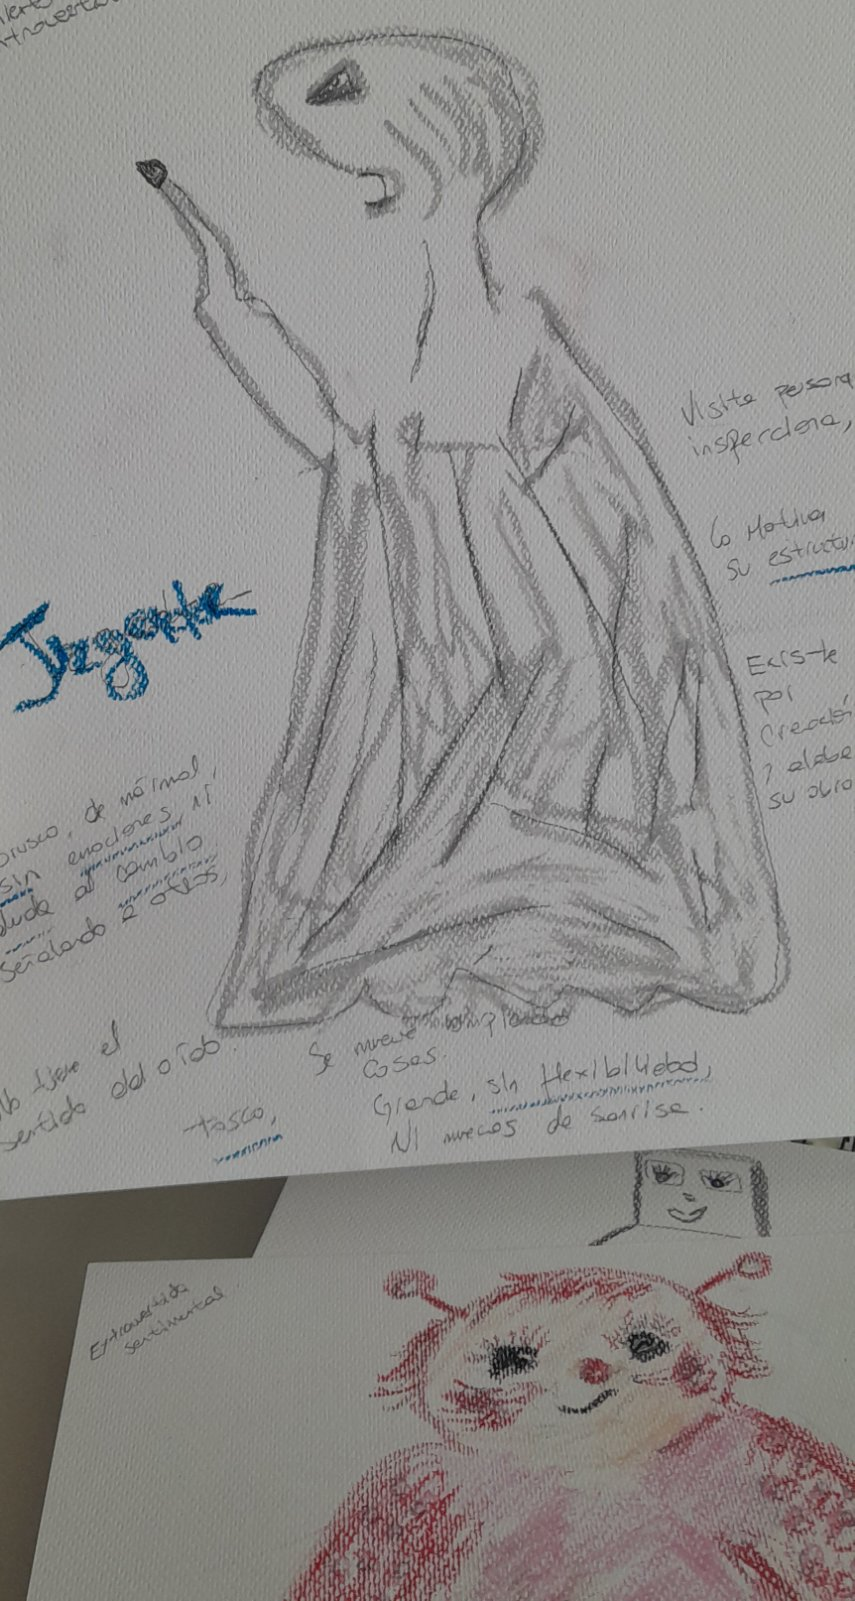
\includegraphics[width=\textwidth]{./images/1f81324df3cf07.jpg}
\end{figure}

\begin{figure}[H]
	\centering
	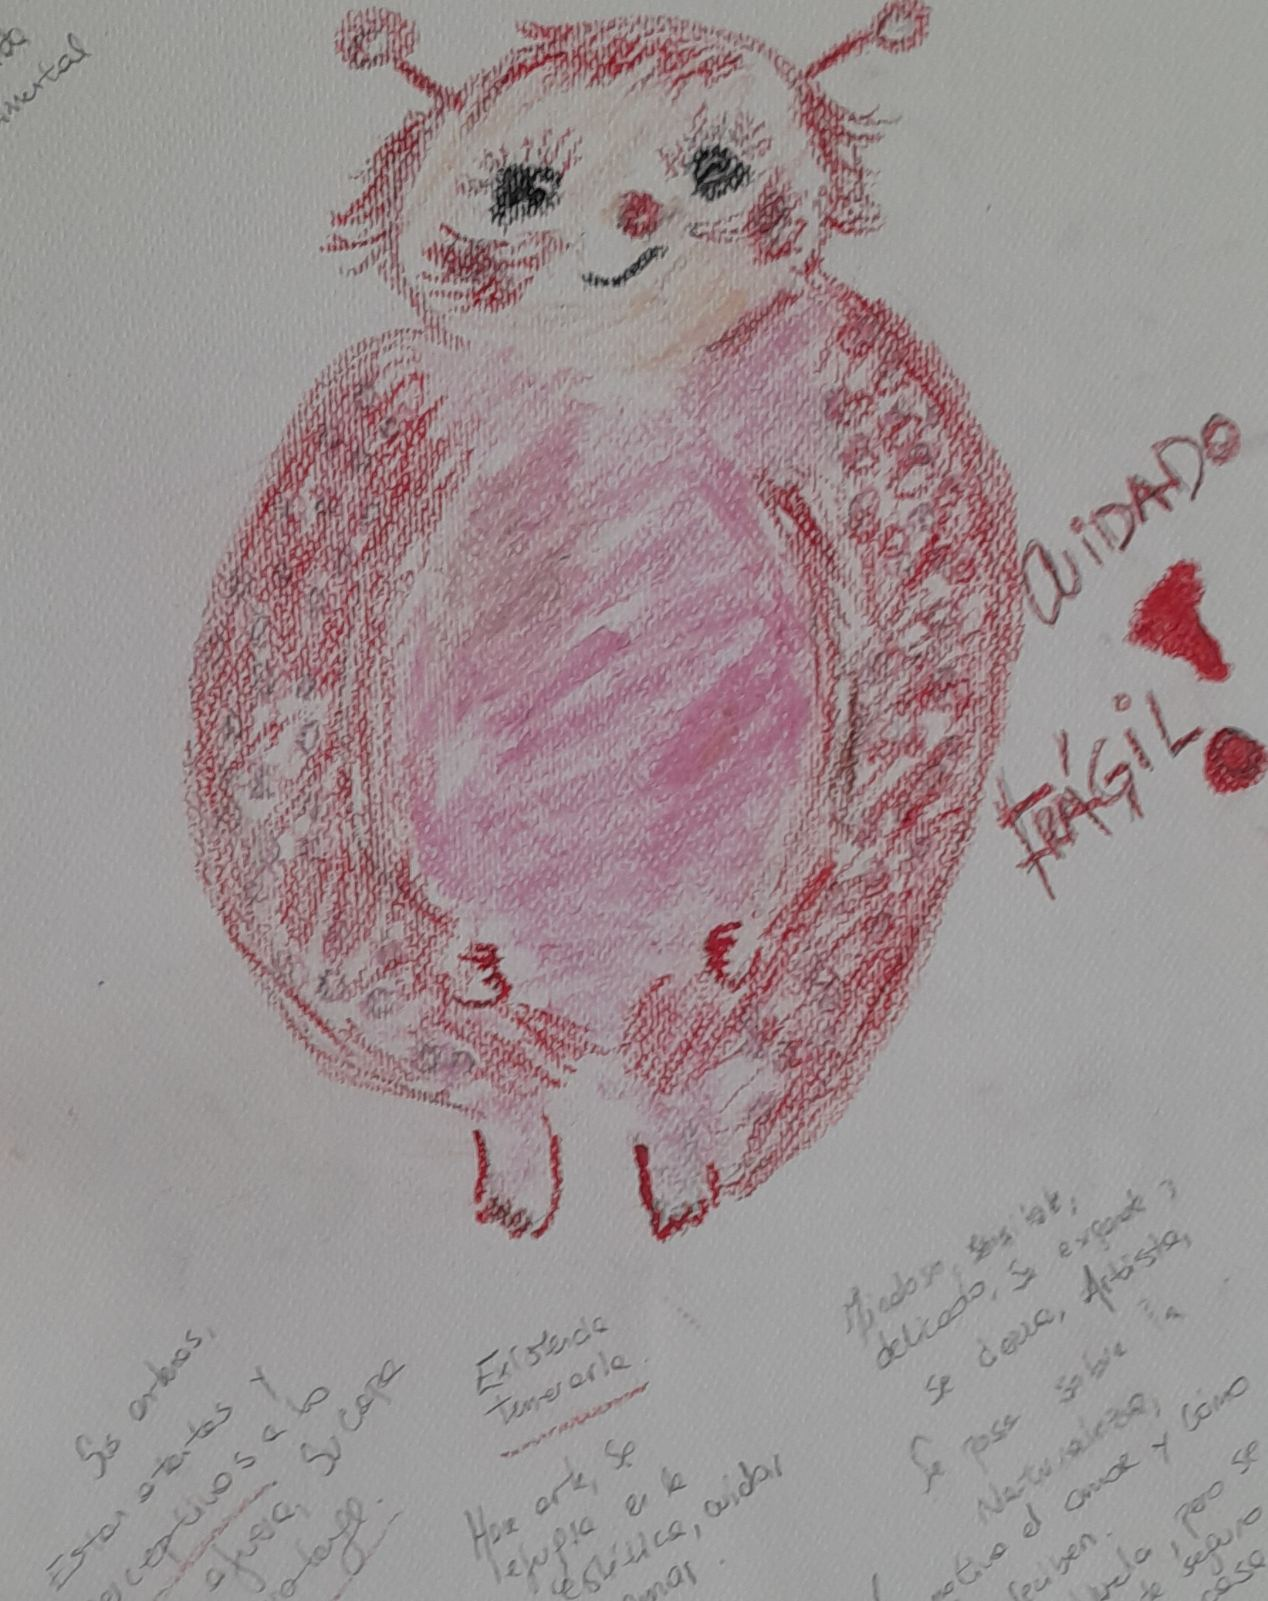
\includegraphics[width=\textwidth]{./images/1f81324df3d3e3.jpg}
\end{figure}

\begin{figure}[H]
	\centering
	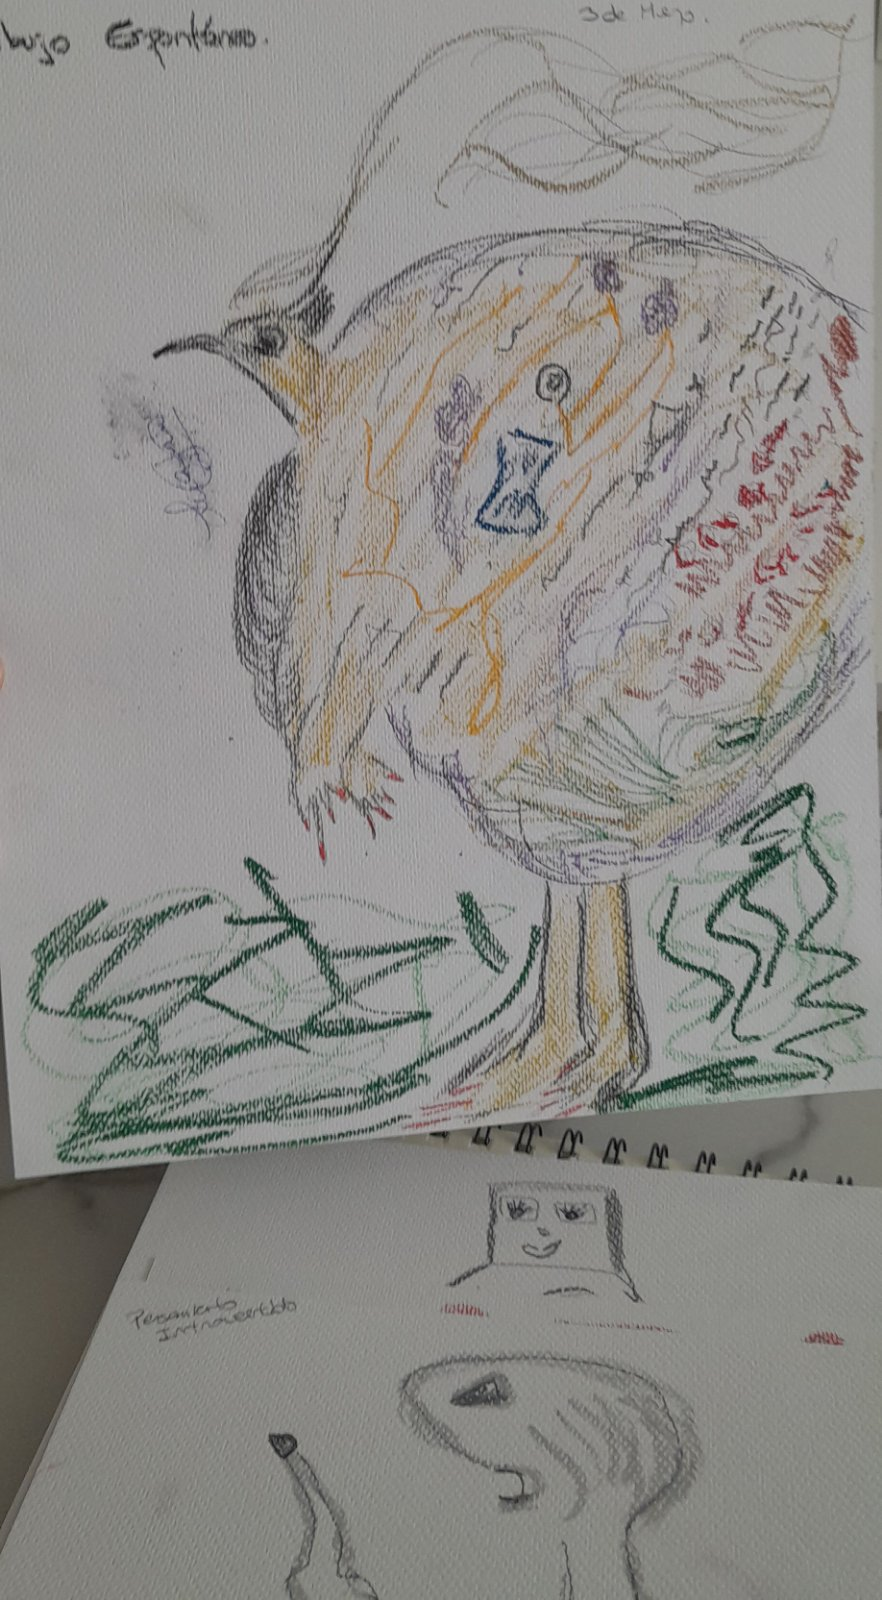
\includegraphics[width=\textwidth]{./images/1f81324df3ff6b.jpg}
\end{figure}

\begin{figure}[H]
	\centering
	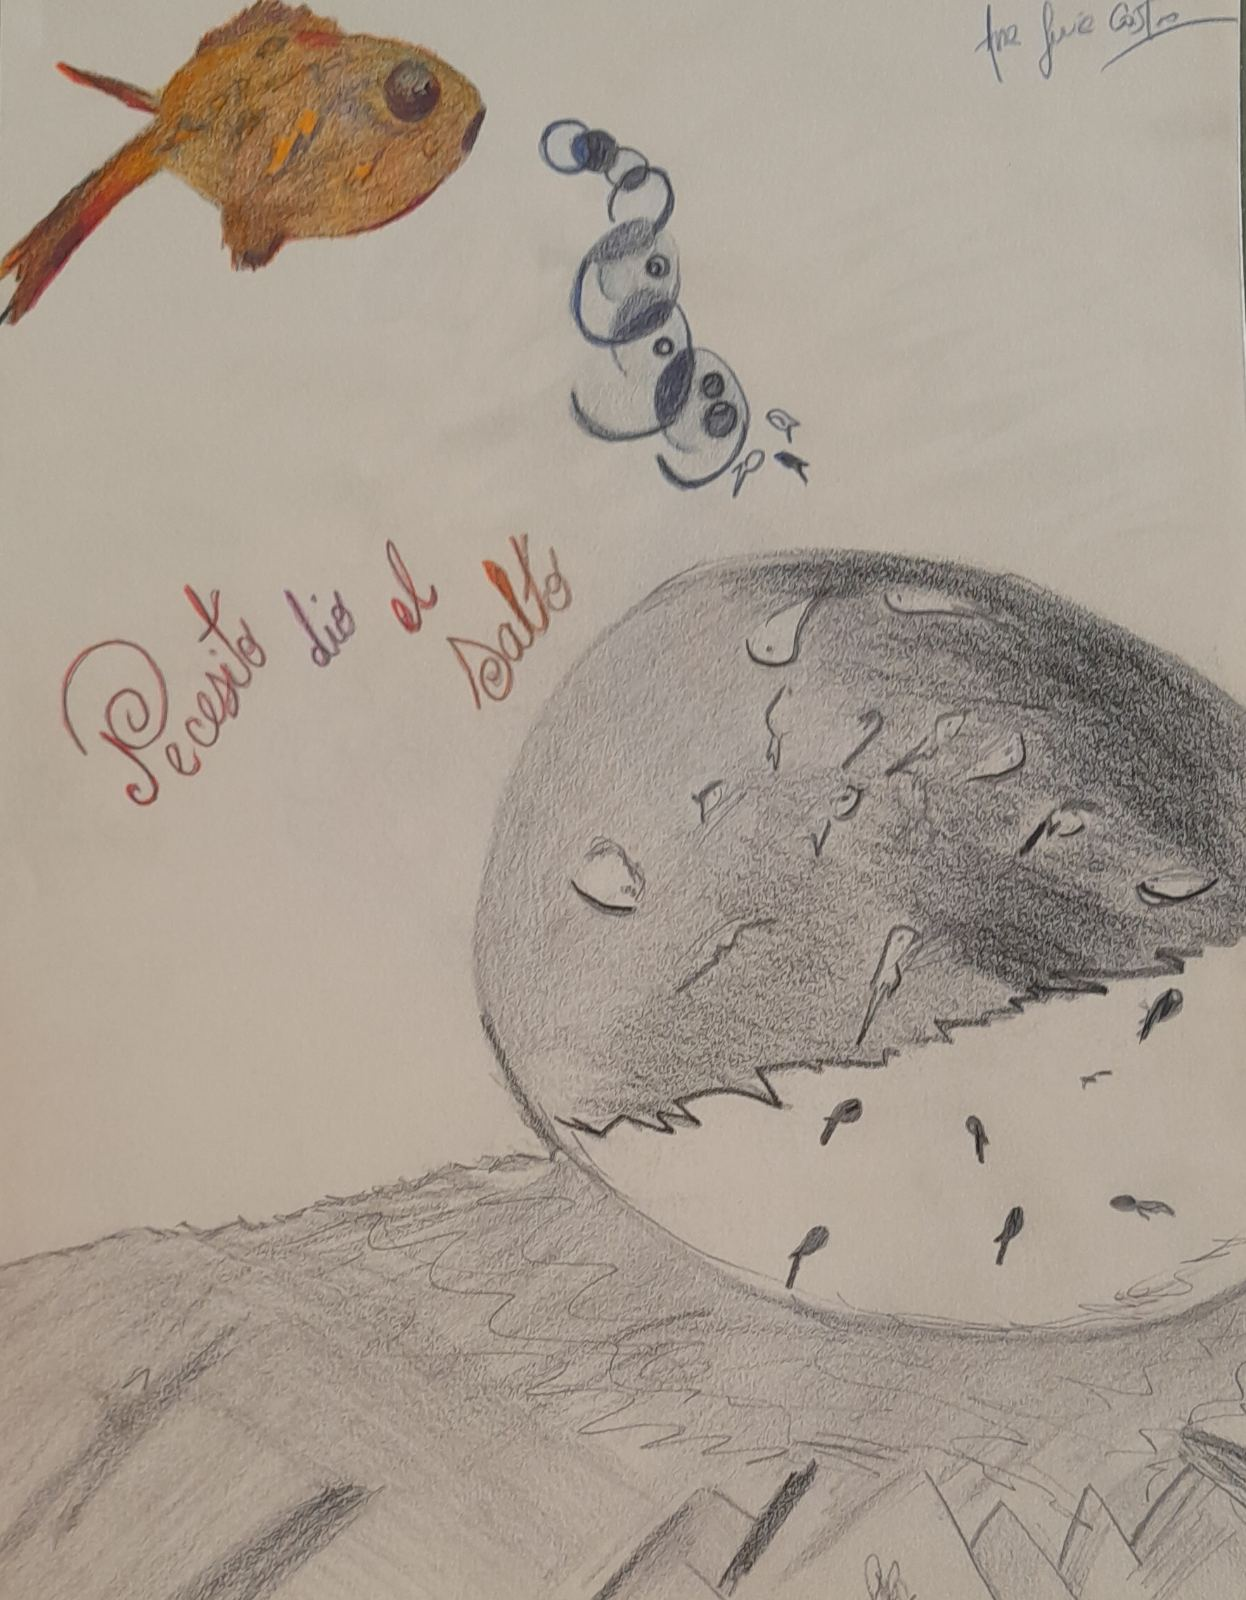
\includegraphics[width=\textwidth]{1f81324df70a75.jpg}
\end{figure}

\clearpage

\noindent\textbf{Integración}\\
Erase una tarde, una de las tantas en que ella salía a explorar, a buscar, a perderse y entre su imaginación volverse a encontrar. Distraída en su mundo interior, sin prisa, puesto que las responsabilidades no eran su premisa. Sin rumbo entre árboles de los que muy bien  historias saben narrar, simplemente era ella, de soñadora eterna encasillada,  la del medio de tres hermanas, con los pies en otro planeta como solían llamarla, así de olvidada Julia caminaba por lugares donde raramente las personas circulaban.
Pero esa tarde, un acontecer muy extraño  pausaria el instante, y ambos, se mirarían sin declararse extraños.
Un pequeño en un mundo gigante, una gigante en un mundo pequeño, cuanta conexión entre ellos.
Cuenta la historia que, como todos los Domingos Lisandro caminaba hacia el río en Lenton, de prisa como todo en su vida, a buscar las monedas del día, con su caña, carnada y su balde, de la rutina un soldado olvidado.
Luego de varias horas sentado en el puente, mirada perdida, del tironeo pendiente, su balde de bagres se ve desbordado, vivos y aleteando los lleva al mercado, donde en lo de Beto se venden muy caros.
Allí viajaba pecesito, entre otros tantos, tal vez nueve que giraban en vano, ni raro ni distinto, con el valor en sus aletas que le dieron el impulso de balancearse y buscar otra oportunidad.
Pecesito se mantuvo respirando en un pequeño charco, de la suerte pasó a un milagro, a medida que este se fue secando, una fuerte tormenta de verano mantuvo, ese lugar sagrado, esos días inundado
Asi es como el encuentro fue desarrollado...
El sol entregaba los últimos rayos y en una botella de cinco litros que  en manos de la pequeña Julia  fueron reflejados, así vio pecesito el aire que ya se le estaba acabando.
Como un tambor, fue un pequeño golpe en su botellón, no podía ella ni  con su más intrépida imaginación creer que se trataba de un pez, no es lo que se suele ver en esa olvidada vía del tren.
Sin titubeos la pequeña niña no dudo en comprender que ese día serían salvados dos partes de un mismo ser que antes de esa forma nadie los había observado, y en el océano de la integración pecesito dio el salto.


% Chapter 6
\chapter{Reintegrarme y entrar en acción}

\begin{figure}[H]
	\centering
	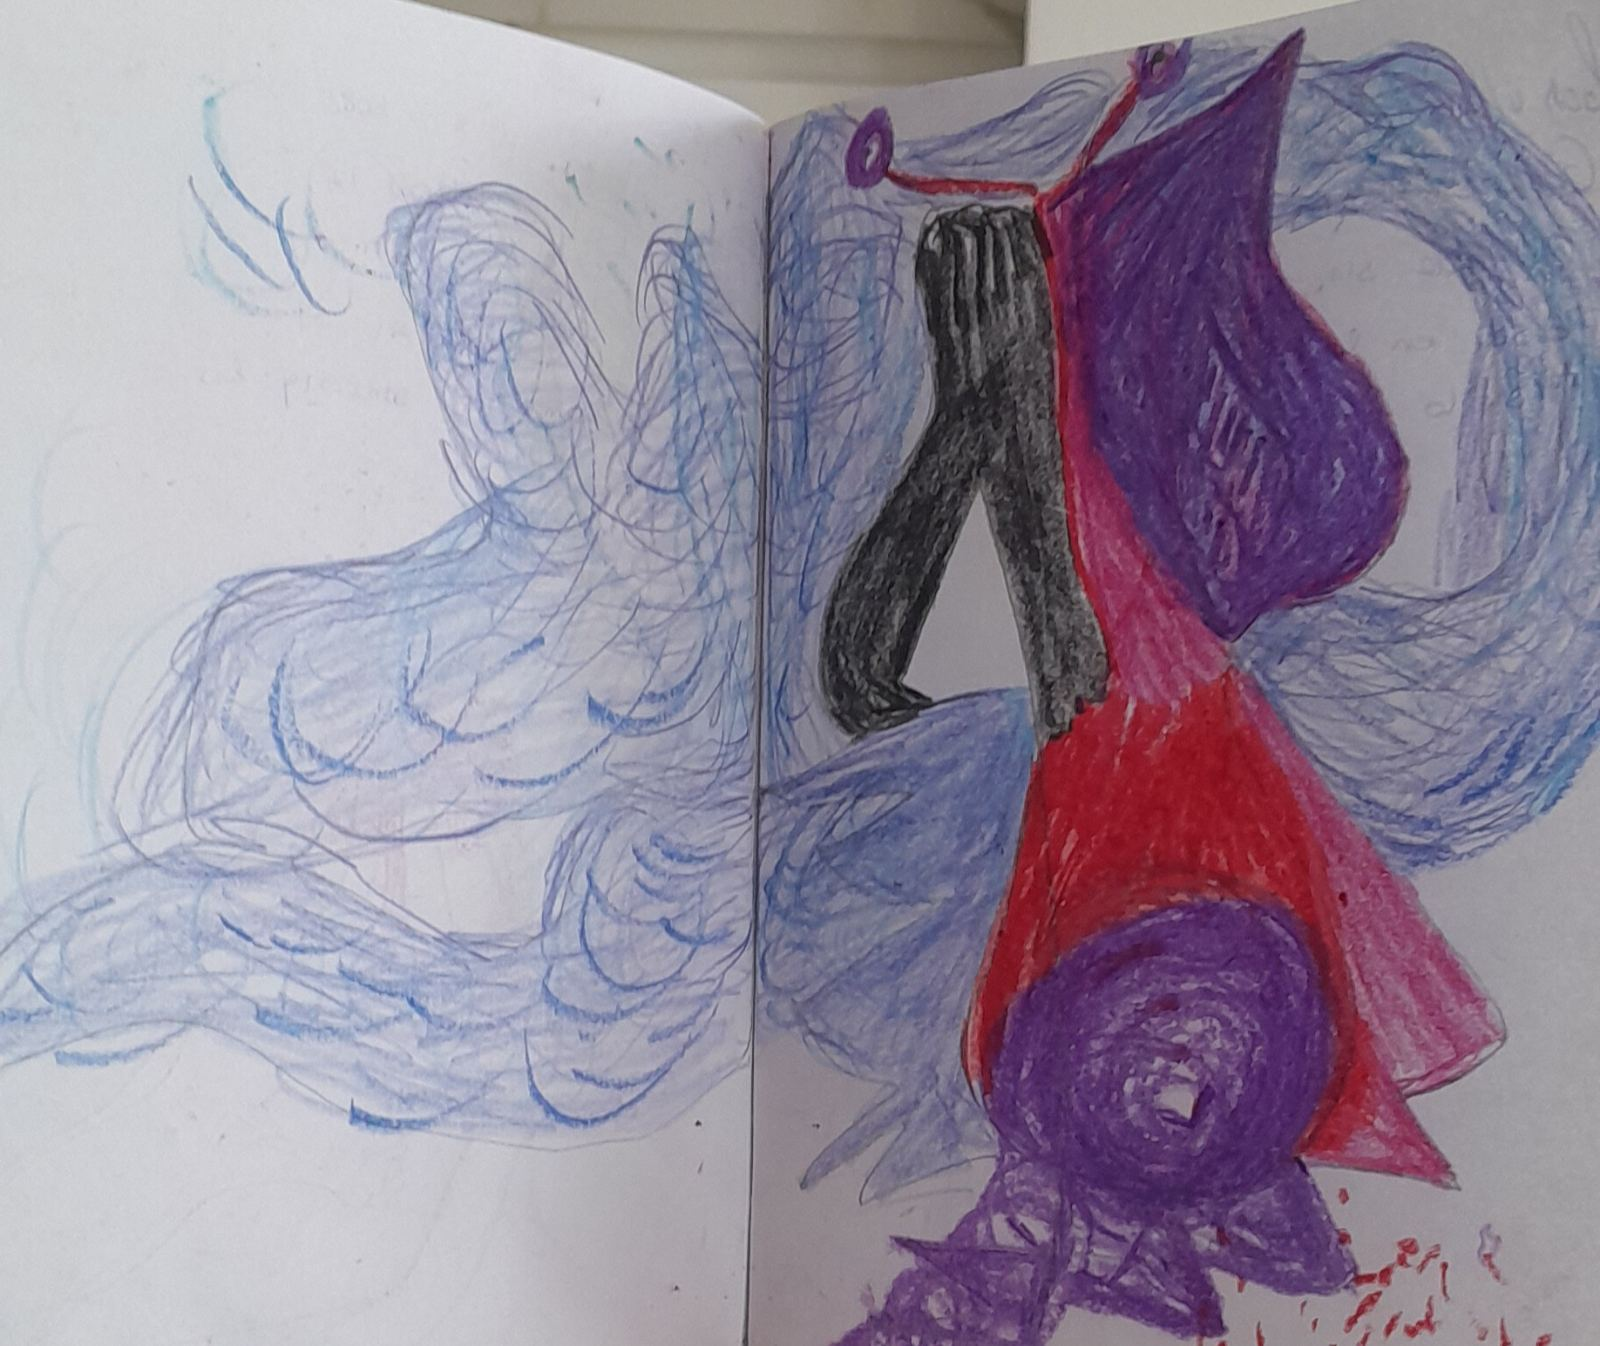
\includegraphics[width=\textwidth]{./images/1f81324df258a4.jpg}
\end{figure}

\begin{figure}[H]
	\centering
	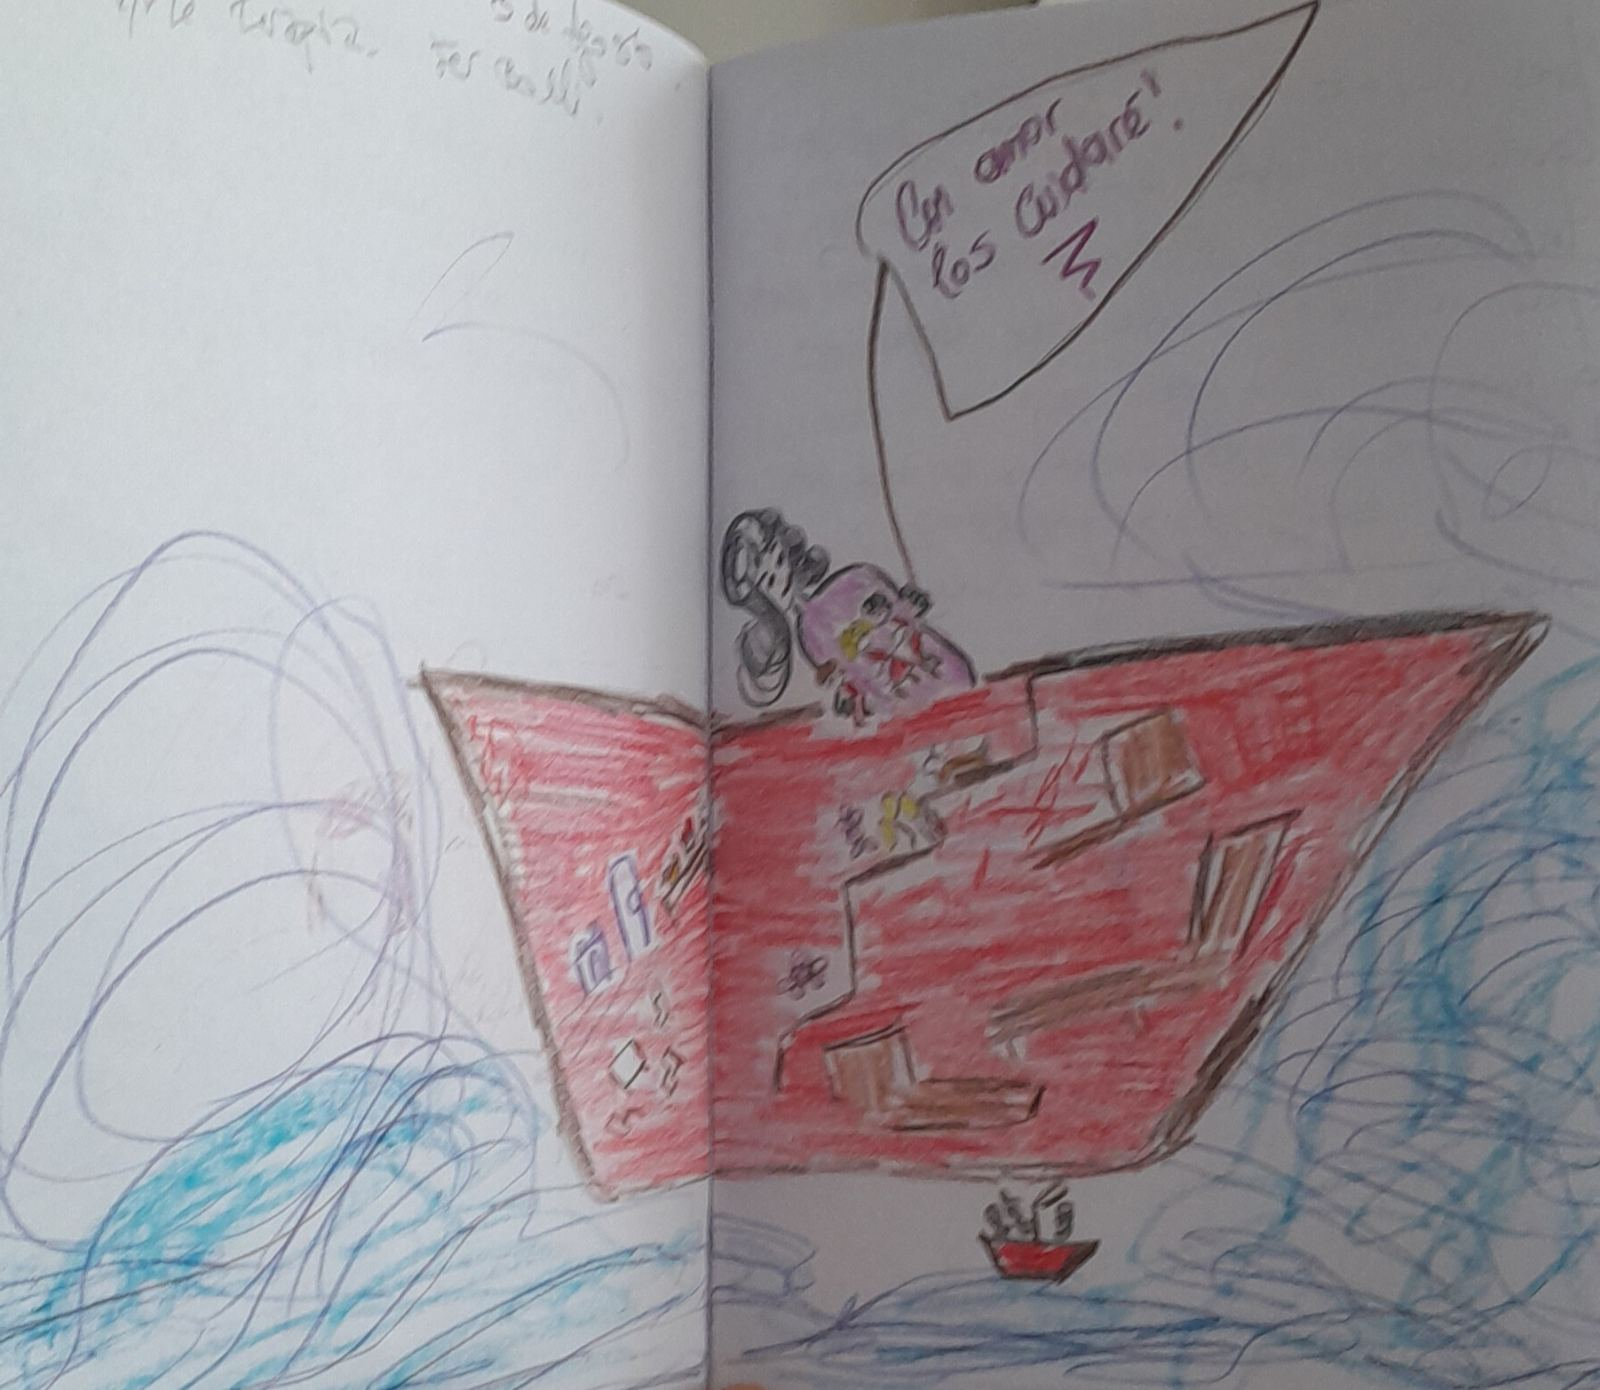
\includegraphics[width=\textwidth]{./images/1f81324df3b99e.jpg}
\end{figure}

\begin{figure}[H]
	\centering
	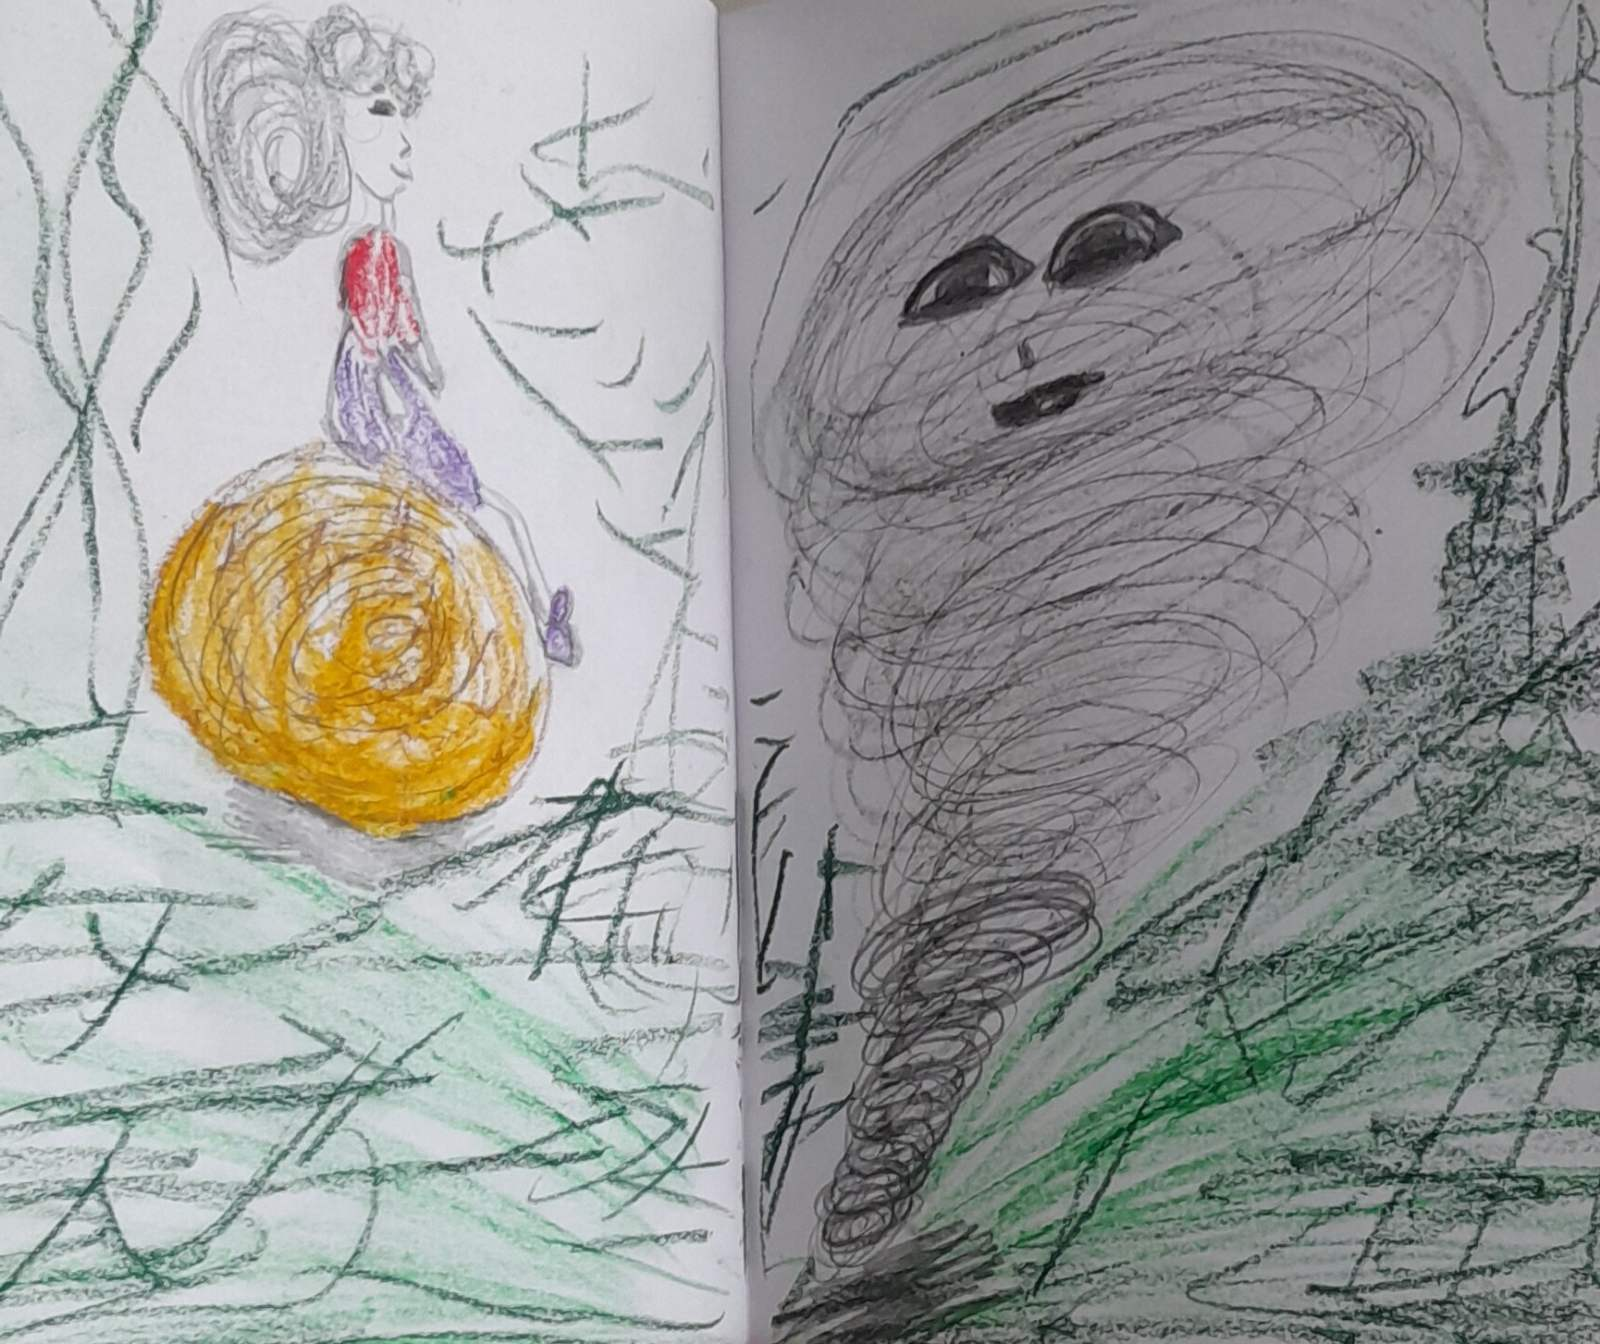
\includegraphics[width=\textwidth]{./images/1f81324df3ed55.jpg}
\end{figure}

\begin{figure}[H]
	\centering
	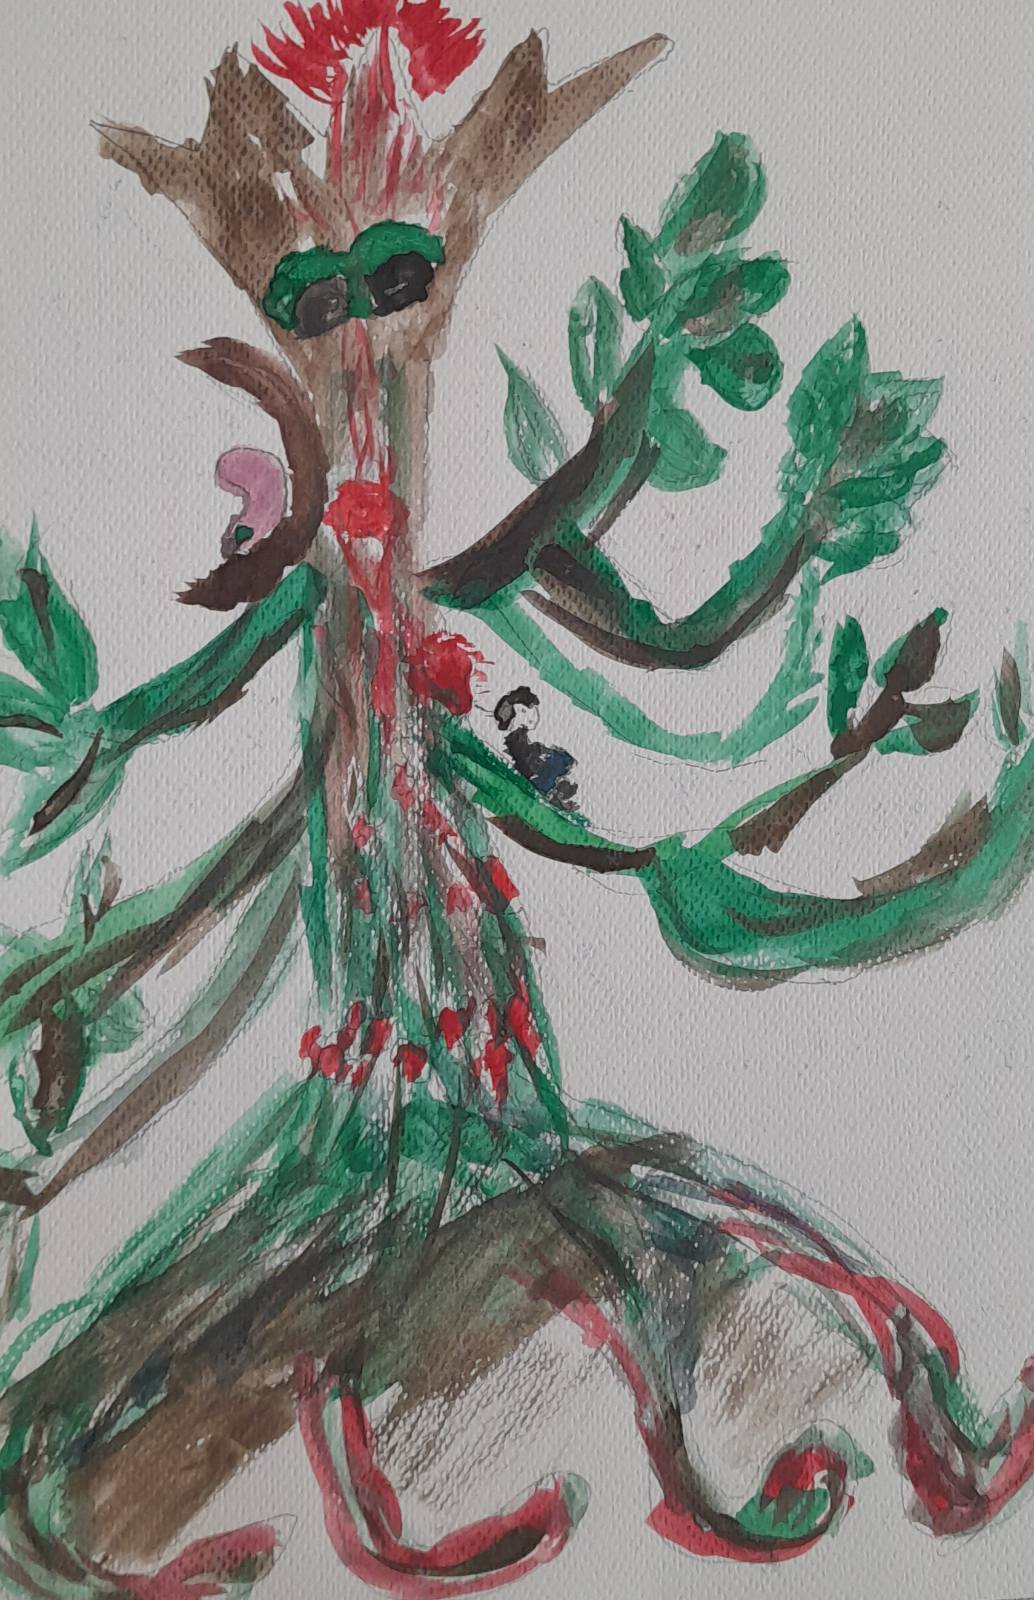
\includegraphics[width=\textwidth]{./images/1f81324df17c98.jpg}
\end{figure}

% chapter 7
\chapter{Gracias por compartir el viaje conmigo}

\noindent\textbf{Bonus literario}\\

\clearpage

\noindent\textbf{Sin ingridientes ni recetarios}\\
Mama quédate tranquila que no estoy sufriendo, me estoy re descubriendo, cambiando espadas por plegarias, a veces sangran y sanan, otras gritan y callan.
Mama hoy estoy llorando, por los momentos que he intentado, elegir entre dos zapatos, respirar lento en la tensión, sentirme comprendido en una discusión, tener la fortaleza de que confían en lo que soy.
Mamá, creo estoy comprendiendo, el zapato que elegí hoy, hasta le cambio el cordón, tomo aire discutiendo, no es mío el descontento, ser fuerte ya no es mi moneda corriente, ser transparente me hace consciente, no busco apoyo de otra voz, no hay empatía que detenga el temblor.
Mama hoy estoy al frente, y tu reflejo está en mi espejo, sigo siendo vulnerable, incomprendida, manipulable, más con los ojos brillantes, por no esconder el parecido, con tu camino recorrido.
Por más momentos solitarios, sin ingredientes ni recetario, con conexiones que schokean, cable directo a la Tierra.
La tierra que es Madre, que escucha, que sabe, esa que a veces golpea, solidifica nuestra existencia.
Por más momentos solitarios, sin ingredientes ni recetario.

\clearpage

\noindent\textbf{Joaquína extravió su lazo}\\
Joaquína extravió su lazo, y al regresar ya no estaba en el mismo lugar.
Pasaron siete primaveras..aún la recuerda como la primera,
Entre esperas y esperas  toca a su puerta, quién tal objeto había encontrado
Traía en su rostro tal pena, una pena de esas que no dan tregua.
No pudo Jacobo aceptar, la invitación de Joaquína, dejando caer el retazo, ni tempestad ni silencio, sólo humanos.
Jacobo no pudo aceptar, la puerta tuvo que cerrar,
Joaquína supo que era en vano,  el lazo, la espera, el pasado..
Historias que no acontecen, que abren camino y se pierden.
Jacobo no pudo aceptar, a su rutina tuvo que regresar, el lazo quedó en las manos de quién tanto lo había llorado.
Historias que no acontecen, que así como nacen se pierden, se pierde como ese amuleto que suerte no trae para ellos.
Jacobo no pudo aceptar, presente no rima con ausente, aunque en rima suene muy coherente.
Un lazo que no fue creado, no reconoce a dos extraños, aunque entre sus manos  haya circulado

\begin{figure}[H]
	\centering
	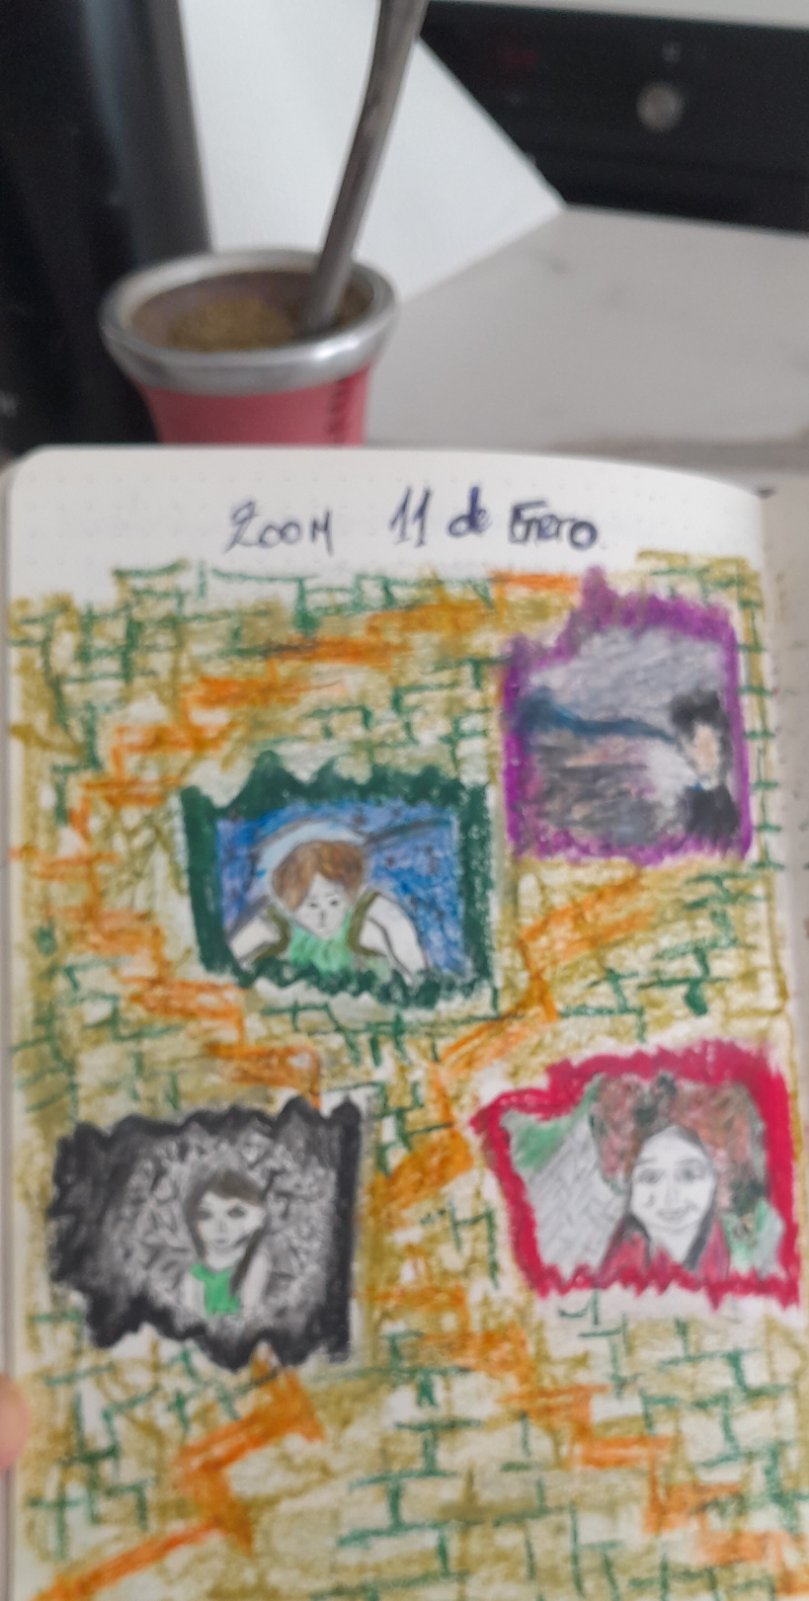
\includegraphics[width=\textwidth]{./images/1f81324ddf1fdd.jpg}
\end{figure}

\end{document}
